% No need to change the first 4 lines of this file
\documentclass{uicthesi}

% This is the user manual for UICTHESI CLS, originally found
% at https://www.math.uic.edu/graduate/current/uicthesi, and
% modified by Pete Snyder <snyder@gmail.com> to match the
% current department requirements.
\usepackage{booktabs}
\usepackage{listings}
\usepackage{newlfont}
\usepackage{amsfonts}
\usepackage{amssymb}
\usepackage{euler}
\usepackage[xindy={glsnumbers=false},nonumberlist,acronym,nopostdot,nogroupskip,nomain]{glossaries}
\usepackage{xspace}
\usepackage[htt]{hyphenat}
\usepackage{float}
\usepackage{flushend}
\usepackage{footnote}
\usepackage{enumitem}
\usepackage{url}
\usepackage{caption}
\usepackage{graphicx}
\usepackage{subcaption}
\captionsetup{compatibility=false}
\usepackage{multirow}
\usepackage{bm}
\usepackage{algorithm}
\usepackage[noend]{algpseudocode}
\usepackage[section]{placeins}
% \usepackage{dsfont}
% \usepackage{xcolor}


\newglossarystyle{clong}{%
 \renewenvironment{theglossary}%
     {\begin{longtable}{p{.2\linewidth}p{.8\linewidth}}}%
     {\end{longtable}}%
  \renewcommand*{\glossaryheader}{}%
  \renewcommand*{\glsgroupheading}[1]{}%
  \renewcommand*{\glossaryentryfield}[5]{%
    \glstarget{##1}{##2} & ##3\glspostdescription\space ##5\\}%
  \renewcommand*{\glossarysubentryfield}[6]{%
     & \glstarget{##2}{\strut}##4\glspostdescription\space ##6\\}%
  %\renewcommand*{\glsgroupskip}{ & \\}%
}

\makesavenoteenv{tabular}
\makesavenoteenv{table}

% See https://www.ctan.org/pkg/glossaries for questions on this package.
% Refer to the acronyms you define here as \gls{nyc}.
%
% This make sure that this text:
%    The Ramones are from \gls{nyc}, thats right, \gls{nyc}.
% Gets output like this:
%    The Ramones are from New York City (NYC), thats right, NYC.
% And that a line in the acronyms section of your thesis has an entry like:
%    NYC         New York City
\newacronym{idot}{IDOT}{Illinois Department of Transportation}
\newacronym{hdp}{HDP}{Hierarchical Dirichlet Process}
\newacronym{dp}{DP}{Dirichlet Process}
\newacronym{ekf}{EKF}{Extended Kalman Filter}
\newacronym{ukf}{UKF}{Unscented Kalman Filter}
\newacronym{ut}{UT}{unscented transformation}
\newacronym{gp}{GP}{Gaussian Process}
\newacronym{rbf}{RBF}{Radial Basis Function}
% \newacronym{eofc}{EOFC}{End of the Century}
\def\new@fontshape#1#2#3#4#5{\expandafter
     \edef\csname#1/#2/#3\endcsname{\expandafter\noexpand
                                 \csname #4\endcsname}}
\new@fontshape{cmr}{bx}{sc}{
      <5>cmcsc8 at 5pt%
      <6>cmcsc8 at 6pt%
      <7>cmcsc8 at 7pt%
      <8>cmcsc8%
      <9>cmcsc9%
      <10>cmcsc10%
      <11>cmcsc10 at 10.95pt%
      <12>cmcsc10 at 12pt%
      <14>cmcsc10 at 14.4pt%
      <17>cmcsc10 at 17.28%
      <20>cmcsc10 at 20.736pt%
      <25>cmcsc10 at 24.8832pt%
      }{}
\mathversion{normal}
\newcommand{\ams}{{$\cal{A}\cal{M}\cal{S}$}}
\newcommand{\amslatex}{{$\cal{A}\cal{M}\cal{S}$-\LaTeX{}}}
\newcommand{\amstex}{{$\cal{A}\cal{M}\cal{S}$-\TeX{}}}
\newcommand{\BibTeX}{{\rm B\kern-.05em{\sc i\kern-.025em b}\kern-.08em
    T\kern-.1667em\lower.7ex\hbox{E}\kern-.125emX}}
\newcommand{\uicthesi}{{$\mathbb{UICTHESI}$}}

\newcommand\bs{\char '134 }   % A backslash character for \tt font
\newcommand{\lb}{\char '173 } % A left brace character for \tt font
\newcommand{\rb}{\char '175 } % A right brace character for \tt font

% one or two other commands
\def\newfont#1#2{\@ifdefinable #1{\font #1=#2\relax}}
\def\symbol#1{\char #1\relax}

\makeglossaries

% Use this file to include custom commands...
\makeatletter
\DeclareRobustCommand{\etc}{%
    \@ifnextchar{.}%
        {etc}%
        {etc.\@\xspace}%
}
\makeatother

\DeclareMathOperator*{\argmax}{arg\,max}
\DeclareMathOperator{\arctantwbo}{arctan2}
\mathchardef\mhyphen="2D
\newcommand{\etal}{\textit{et al}.}
\newcommand{\ie}{\textit{i}.\textit{e}.}
\newcommand{\eg}{\textit{e}.\textit{g}.}
\newcommand{\rpm}{\sbox0{$1$}\sbox2{$\scriptstyle\pm$}
  \raise\dimexpr(\ht0-\ht2)/2\relax\box2 }
\begin{document}

% The title of the thesis
\title{Learning Camera-specific Semantic Knowledge for Surveillance Traffic Analysis}

% Your full name
\author{Yanzi Jin}

% Mention all degrees you hold currently
\pdegrees{B.A., Dalian University of Technology}

% Probably no need to edit this
\degree{Doctor of Philosophy in Computer Science}

% Add your committee members, one per line, mentioning external universities
% where relevant
\committee{Jakob Eriksson, Chair and Advisor \\
	Xinhua Zhang \\
	Brian Ziebart \\
    Jie Yang, MSCS Department\\
    Ahmet Enis Cetin, ECE Department}

% No need to make any changes to the next 10 lines
\maketitle
\copyrightpage 
\dedication

Dedicated to my parents and sister, for their unconditional love and support.
\acknowledgment

% A page or two so of shout-outs to people you appreciate.  Don't forget
% your advisor and committee members!
I want to thank my advisor Dr. Jakob Eriksson throughout these years for his support and instructions.
He is very visionary about this exciting and challenging project. 
I admire his academic attitude and the effort he spent to learn together with students.
I appreciate the time that we went through the code line by line for a hidden bug or hours of discussion of algorithm details. 
Thanks to his generous freedom and support, I received comprehensive training and became independent and mature in research.

Also, I would like to express appreciation to my committee members, for their advice and inspiration. 
I took their classes and learned preliminary knowledge of different research areas, contributing to the building blocks of my research project. 
Specifically, I want to thank Dr. Xinhua Zhang, whose rigorous attitude toward research and passion of teaching greatly inspired me. 
Also, Dr. Jie Yang's rich experience gave me helpful guidance on multiple technical questions.

In addition, I want to thank my parents and sister.
My father teaches me to be strong and tough; my mother supports me for all my big decisions; my sister takes care of my parents when I am far away.
Finally, special thanks to Sihong Xie, for his company and encouragement along this tough journey. 
% This line is required, but of course, replace my initials with yours.
\initials{YJ}
\authorcontributions

% This section should give a rough overview of each chapter in the thesis,
% highlighting your contributions.  Most importantly, for each one of your
% papers you are quoting, this section should briefly describe what each author's
% role / contribution was.

% An example of ``Contribution of Authors'' section is on page 3 of the
% University's guide to iThenticate\footnote{\url{http://grad.uic.edu/sites/default/files/pdfs/Introduction_to_Screening_Your_Thesis_or_Dissertation_using_iThenticate-final_a.pdf}}.

Chapter \ref{chp:tracker} represents a published manuscripts with complete citation, where I am the first author.
My advisor Jakob Eriksson contributes to the writing of it.
Other parts of this thesis consists of my own unpublished experiments.
\tableofcontents
\listoftables
\listoffigures
\printglossary[type=\acronymtype,title=LIST OF ABBREVIATIONS,style=clong]
\summary

% One to two page summary of the entire work.  Like a long abstract.
As the reduced manufacturing cost of camera brings the prevalence of surveillance camera, people are putting more effort on efficient information retrieval from surveillance videos.
On the other hand, surveillance videos are becoming a separate subject for academic study, due to their spacial features and wide applications.
However, there remains a huge gap between academic computer vision research and application. 
Parties in the possession of a large amount of videos lack systematic methodology for different tasks;
while the research community has little access to data with the same amount and complexity real-world data, algorithm performance also has a higher priority over practical bottlenecks in real-world application, such as throughput and automation.

This thesis aims to bridge the gap between the state-of-the-art computer vision research and real-world application.
We first address the critical problem of proper initialization and termination in object tracking algorithm, and propose a heuristic method for automatic initialization and termination.
Then we work on learning the scene-specific semantic knowledge and apply them for other surveillance tasks such as vehicle tracking and counting.
We demonstrate the performance improvement by the heuristic method and further boost by the semantic knowledge.

With feasibility for real-world deployment being the prerequisite, our methods are end-to-end without human input and run in real-time. 
Finally, we annotate and release a comprehensive dataset for the community. 

% This is where you write the paper.  I've included a sample chapter
% below, to suggest a possible organization.  Just add references to the
% rest of your paper here.
\chapter{Introduction}
\label{chp:intro}

\section{Camera system for traffic engineering}
\label{sec:intro-its}

% Surveillance infrastructures generate vast amounts of data which, if effectively analyzed, provide huge potential for informing decision making.
% A shopping mall may use the statistics of customer visit count and average shopping time to analyze sales performance; 
% surveillance records may provide evidence to the police and help solve criminal cases;
% urban planners may use traffic flow data to develop better traffic patterns.
Vehicles on the road generate vast amounts of data which, if effectively analyzed, provide huge potential for informing decision making.
In traffic engineering, urban planners use traffic flow data to develop better traffic patterns.
The standard method for collecting data involves manual counting people by a field agent.
For vehicles on the road, equipment such as pressure tubes laid across the pavement, magnetic loops under the pavement \cite{klein2006traffic,mimbela2000summary} is used to collect data, but it is hard and expensive to set up and maintain.

On the other hand, the cost of cameras continues to decrease, therefore, deploying a camera system rather than traditional equipment becomes an obvious choice.
The wide deployment of cameras leads to better coverage of the city, but also a massive amount of video data.
The essential task for image-based data collection is extracting and efficient indexing of desired data.
Currently, such tasks still primarily rely on eye-balling the interested object or event, which is inefficient.
Fortunately, computer vision is becoming powerful and approaching human performance on some problems.
People tend to seek more cost-efficient solution of traffic flow analysis via computer vision.
With the computational advantage, computer vision techniques are expected to cut the cost and scale up those tasks.
\section{Computer vision in transportation}
\label{sec:intro-cv}

With the progress in artificial intelligence and higher demand in its application, computer vision is becoming one of its hottest sub-domains. 
Computer vision enables computers to perform tasks that human is good at, such as visual detection and tracking. 
With the superior advantage of computational speed, these tasks can be applied in large scale.

When the fundamental theory of this field has become rather mature, researchers gradually shift their attention to more specific tasks and data. For example, pedestrian detection \cite{dollar2012pedestrian} and face recognition \cite{parkhi2015deep}, gesture recognition \cite{rautaray2015vision} has become individual topics due to their huge application potential and high demand.
On the other hand, transportation videos have also drawn much attention because of the various practical challenges and the huge impact of applications in the intelligent system field. 
Researchers are studying the computer vision problems specific to traffic videos, such as anomaly detection \cite{scime2018anomaly}, tracking \cite{wu2015object} and counting \cite{seenouvong2016computer}. 

The videos from traffic cameras have a few unique features: 
\begin{itemize}
\item They are recorded ceaselessly, therefore, in large quantity; 
\item They are usually of low-resolution quality due to the transmission and storage limits;
\item They have a special composition (pedestrian and vehicle) and the objects in the view move in a regular motion pattern.
\item Depending on the location, the video may contain a large number of objects with highly complex interactions.
\end{itemize}

Therefore, the complexity of the videos and the high-performance requirement raise challenges for robust intelligent transportation systems. 
Ideally, they are expected to perform the task with one-time setup and the minimal amount of human effort, with high accuracy and high speed.
\section{Practical visual surveillance}
\label{sec:intro-surveillance-cv}

While people in both civil engineering and computer vision are working toward the same goal --- building the real-world visual surveillance systems, there is still a big gap between the state-of-the-art research and the practice use.
Researchers in academia need an in-depth study of a specific problem; therefore, they usually make simplified assumptions to isolate the problem and ignore the impact of other factors. 
However, the real-world application runs in a complex environment and deals with noisy data. Data cleaning and processing speed have to be taken into account.
For example, researchers care more about the novelty and performance of the solution and assume the computation resources are unlimited. 
In this case, even though some algorithms outperform human, they are too slow to process a massive amount of data. 
Besides, academic problems usually have a standard benchmark with well-processed data, so that people could spend the minimal amount of time on evaluation, with a uniformly acknowledged standard.
However, those data might be too small and ideal compared with the real-world data, and the evaluation metric may not be comprehensive for those complex and noisy data for different tasks.

After some failed trails of computer vision algorithms on data from the local department of transportation, it turns out that noisy data is one major obstacle for processing real-world data. 
Besides, minimal human input and real-time processing speed is the prerequisite for large scale application.
On the other hand, there lacks a standard benchmark and dataset for the researchers in the field to study the visual surveillance problems and solve the bottleneck problem.

In this thesis, we try to address the aforementioned problems neglected in visual surveillance field and narrow the gap between the computer vision research and large scale application. 
Specifically, we are building an end-to-end pipeline for transportation video analysis, minimizing human input and maximizing the throughput.
We aim to solve the problems in vehicle tracking and counting that are critical to the performance, such as automatic tracking initialization/termination, noise elimination.
On top of that, we try to further improve the algorithm performance by learning semantic knowledge in an unsupervised manner, taking into account that the regular vehicle motion pattern from a static camera could be informative for analytic tasks.
Through comprehensive experiment and case studies, we show that proper initialization and termination improves the performance of the general automatic tracking framework with any tracking algorithm; and the semantic knowledge brings more benefits to multiple visual surveillance tasks.
As a by-product of our experiment, we annotate and release a large dataset for the community \cite{yanziVehicleTracker}, aiming to attract and help more researchers to work on such problems.

\chapter{Fully Automatic Vehicle Tracker}
\label{chp:tracker}

\section{Introduction}
\label{sec:tracker-intro}

Vehicle tracking has important applications in traffic engineering.
Over time, a number of vehicle counting methods have been developed, including specialized hand-held counting boards with buttons to push, pressure tubes laid across the pavement, magnetic loops under the pavement \cite{klein2006traffic,mimbela2000summary},
video-based lane occupancy detectors, and more. 
Overall, the most powerful techniques rely on manual input and tend to be extremely labor intensive, whereas the mostly automatic techniques lack in accuracy and descriptiveness.
In principle, computer vision provides the most scalable and economical alternative. 
Ideally, a fully automatic computer vision-based tracker follows each vehicle as it enters, traverses and exits the scene.
% In principle, computer vision promises an alternative that is both highly descriptive and fully automatic, using existing, arbitrary-perspective traffic video. 
%By automatically following each vehicle as it enters, traverses and exits the scene, then classifying the resulting trajectory, a computer vision system could in principle count an arbitrary number of vehicle movements, on a continuous basis, at very low cost.
However, current tracking algorithms such as \cite{henriques2015high,vojir2014robust,hare2011struck,possegger2015defense} all require initialization as input, leading to semi-automatic tracking systems. 
To avoid manual input, these trackers rely on background subtraction and/or object detectors for initialization. 
Here, the primary challenge is robustness to variations in illumination condition, viewpoint, and video quality. 
Background subtraction model can fail with illumination change, while detectors are not appropriate for detecting a vehicle in the distance, or in a grainy low-resolution video, as our experiments demonstrate. 
Additionally, the low throughput of most trackers prevents widely deployed visual applications, as VOT 2016 challenge reports that none of the top-ranked trackers run in real-time for even a single tracked object.

% The primary challenge is robustness to variations in viewpoint and video quality. Current work on object tracking \cite{henriques2015high, vojir2014robust, hare2011struck, possegger2015defense}, generally assume that initialization is provided. That is, one of the inputs to the tracker is the initial location and extent of the object to be tracked. General purpose, automatic initialization is not well covered in the literature, however an object detector can be used in its place. In our experience with one state-of-the-art detector \cite{renNIPS15fasterrcnn}, this approach works best with a clear, high-resolution view of the object. Thus, current detectors are not appropriate for detecting vehicle in the distance, in a grainy low-resolution video. Many similar challenges apply to other isolated approaches to object tracking in this context. 

In this chapter, we propose a fully automatic algorithm for vehicle tracking that runs faster than real-time. 
With a sensor fusion approach, we combine background segmentation, object detection, and optical flow into a single, robust vehicle tracking system via Kalman filtering. 
Initialization uses the same three sources, to automatically identify moving objects in the scene. 
Finally, when an object exits the scene, its movements are analyzed to filter out unlikely object trajectories.
To evaluate our algorithm as well as prior work, we create a hand-annotated dataset, consisting of 11 diverse, 5-minute videos collected from existing traffic cameras. 
For each frame, the location and extent of each moving object is provided, which enables accurate, quantitative evaluation.

We also compare the proposed algorithm against multiple state-of-the-art trackers, which rely on human input for initialization.
On this dataset, we report considerably better performance than the state of the art with manual initialization, and substantial accuracy improvement when using our new automatic initialization method. 
Moreover, we demonstrate throughput 4$\times$ faster than real time and over 5$\times$ improvement compared to 5 out of 7 several baseline trackers, up to 47$\times$. 

%The primary contributions of this paper are summarized as follows:
%\begin{itemize}
%   \setlength\itemsep{0pt}
%   \setlength{\parskip}{3pt}
%   \item Robust automatic tracker initialization and termination.
%   \item Efficient framework to integrate optical flow, background subtraction model and object detector for automatic vehicle tracking.
%   \item Public release of fully annotated traffic video dataset containing 11 real-world videos with different views, resolutions, illumination conditions and vehicle interactions, plus source code for our vehicle tracking system, to be released upon publication. 
%   \item Thorough evaluation on each component of our framework and comparison with a state-of-the-art object tracker. 
%\end{itemize}


%Our paper is organized as follows: \S\ref{s:preliminary} illustrates several common vision techniques used in tracking. with detailed example we demonstrate that none of those methods are practically reliable under real-world conditions, however, complimentary in some sense. \S\ref{s:method} describes our sensor fusion method that combines three unrealiable into a robust system, with stress that tracker initialization and termination should be carefully dealt with. Fianlly, in \S\ref{s:evaluation} we present comprehensive evaluation, extensively on our ready-to-release video dataset with complex adversarial conditions. By comparison with sveral state-of-the-art trackers, our fully automatic tracker shows substantial performance improvement and huge potential for scalable use in traffic engineering.


%Object tracking has been studied in computer vision field for decades with great progress most recently. However, there is still gap between algorithms and real world applications. Researchers often simplifies some conditions to better focus on a certain problem, while practical systems have to take every component in the work flow into account. As an inevitable step for tracking, initialization is seldom explicitly addressed in current literature. Different with manual labeling in standard tracking evaluation, people use background subtraction and object detector to initialize trackers automatically in real world systems. Although these components are usually assumed perfect in literature, exceptions do exist in reality. Background subtraction fails with illumination change and occlusion, while object detector usually has missing and false detections.
%Besides source of initialization, we argue that the moment of tracker initialization and termination is key to the performance. We want an accurate trajectory as long as possible, while accuracy and coverage in time is contradictory sometimes.

%-------------------------------------------------------------------------
\section{Preliminary}
\label{sec:tracker-preliminary}

The problem of vehicle tracking in existing traffic surveillance video presents some unique computer vision challenges, including scale changes, video quality (exposure control, automatic white balance and compression), weather conditions, illumination changes, variations in perspective, and occlusion.
Current work in object detection 
\cite{viola2001rapid,dalal2005histograms,felzenszwalb2010cascade,girshick2014rich}, 
tracking \cite{henriques2015high,hare2011struck,vojir2014robust}
and background subtraction \cite{barnich2011vibe,zivkovic2006efficient}
% \cite{barnich2011vibe, zivkovic2004improved, zivkovic2006efficient, wang2007consensus} 
can deal with a subset of these conditions, but so far a generic system has been elusive. Below, we first introduce the underlying methods used in our system, then describe our vehicle tracking framework in detail. 

%We are inspired by the observation that object detector and background subtraction are complementary in some sense. Background subtraction model is able to catch small moving object but sensitive to illumination change and occlusion; on the contrary, object detector is robust to lighting and occlusion change, while prone to miss small object. Meanwhile, motion is a key evidence when appearance is not reliable and able to be computed efficiently as optical flow. We are trying to build a generalized form to combine these components into a reliable framework.

%-------------------------------------------------------------------------
\subsection{Background subtraction}
Background subtraction generates a binary foreground mask given a sequence of frames. Connected areas in the foreground mask can be treated as moving objects, although this technique can be error prone. 
We use ViBe \cite{barnich2011vibe}, for its balance of speed, robustness and accuracy. However, other methods 
% including \cite{stauffer1999adaptive, kaewtrakulpong2002improved,zivkovic2004improved,godbehere2012visual,kumar2000foreground, javed2002hierarchical,elgammal2000non,zivkovic2006efficient,wang2007consensus} 
can be substituted with acceptable results in many cases.

\ref{fig:tracker-bg} summarizes four common failure cases of the background subtraction with foreground bounding boxes on the original frame on the left and the foreground on the right. Automatic exposure (Figure \ref{subfig:bg-autoExposure}) is performed by the camera during recording, whereas illumination variation (Figure \ref{subfig:bg-illuminationChange}) is due to external light sources, such as the sun and vehicle headlights.
Both automatic exposure and illumination variation cause rapid and widespread changes in pixel values, which most background subtraction methods struggle with. 
Occlusion (Figure \ref{subfig:bg-occlusion}) creates a single connected foreground area out of two or more moving objects, or sometimes multiple foreground areas for a single moving object, breaking any assumption of a one-to-one mapping between foreground areas and moving object.
Ghosting (Figure \ref{subfig:bg-ghost}) usually happens when a foreground object remains stationary for a long time, during which time it is gradually assimilated into the background model.
When the object begins to move, what appears from behind the object is inaccurately marked as foreground, until the background model has had time to adjust.
% To make matters worse, it can take a long time for the model to correct this mistake, depending on the model's rate of adaptation, and the content of the video. 
%Once the background model fails, it is hard to extract the real moving object since it is just a pixel-level operation.
%, extra information like edge \cite{st2015subsense} and texture \cite{st2015self} may help to improve robustness. 
\begin{figure}[!htbp]
\centering
    \begin{minipage}{0.96\columnwidth}
        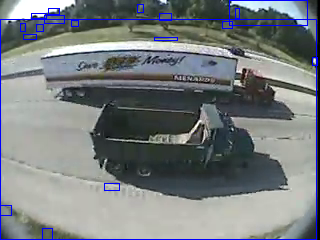
\includegraphics[width=0.48\linewidth, height = 0.3\linewidth]{./img/bg/252707.png}
        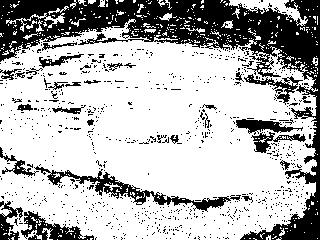
\includegraphics[width=0.48\linewidth, height = 0.3\linewidth]{./img/bg/252707_FG.png}
        \subcaption{Camera auto-exposure.}
        \label{subfig:bg-autoExposure}
    \end{minipage}
    \hspace{0.02\columnwidth}
    \begin{minipage}{0.96\columnwidth}
        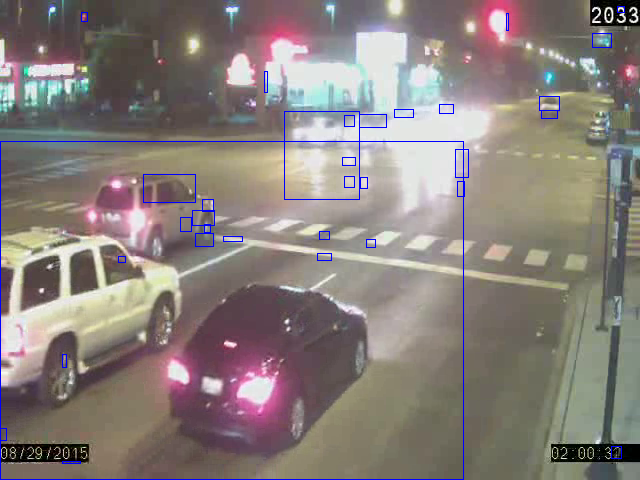
\includegraphics[width=0.48\linewidth, height = 0.3\linewidth]{./img/bg/ciceroPeterson.png}
        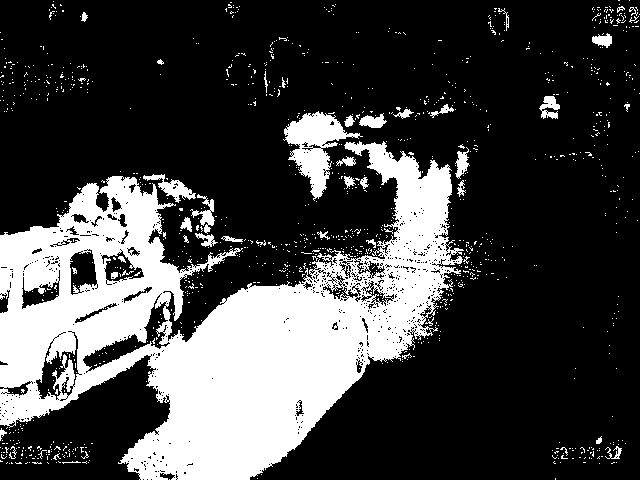
\includegraphics[width=0.48\linewidth, height = 0.3\linewidth]{./img/bg/ciceroPeterson_FG.png}
        \subcaption{Illumination change.}
        \label{subfig:bg-illuminationChange}
    \end{minipage}
    \vfill
    \begin{minipage}{0.96\columnwidth}
        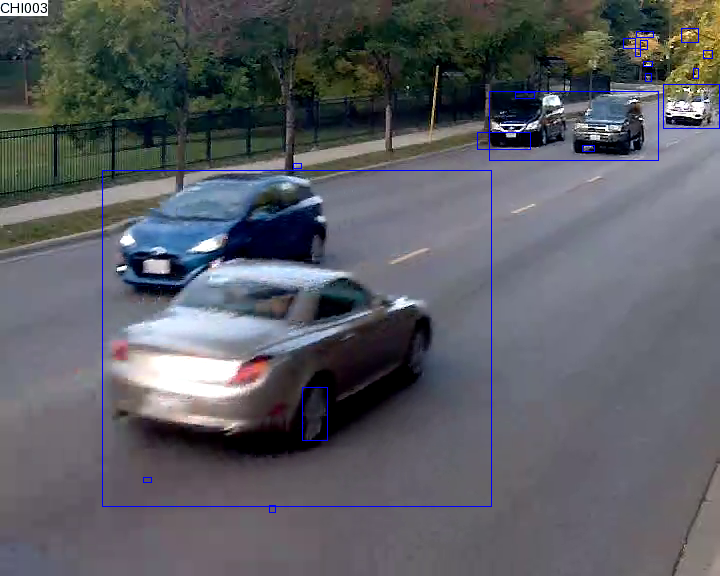
\includegraphics[width=0.48\linewidth, height = 0.3\linewidth]{./img/bg/ILCHI_CHI003.png}
        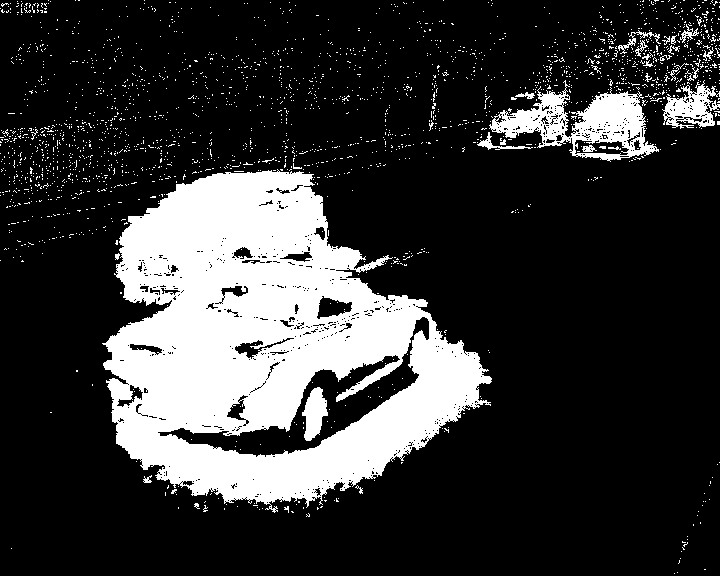
\includegraphics[width=0.48\linewidth, height = 0.3\linewidth]{./img/bg/ILCHI_CHI003_FG.png}  
        \subcaption{Occlusion. Note also the shadow, due to illumination change.} 
        \label{subfig:bg-occlusion}
    \end{minipage}
    \hspace{0.02\columnwidth}
    \begin{minipage}{0.96\columnwidth}
        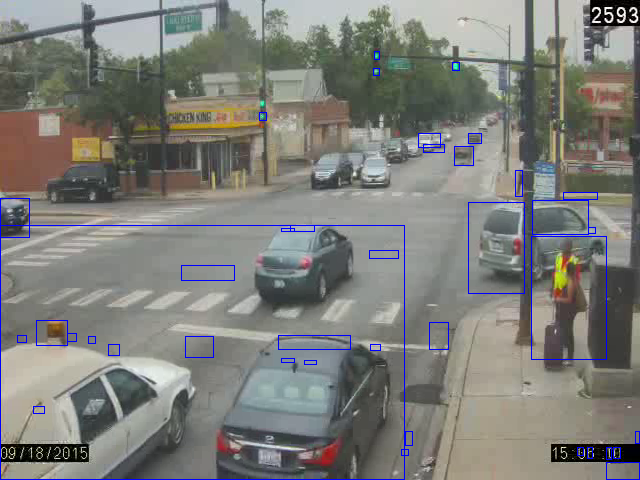
\includegraphics[width=0.48\linewidth, height = 0.3\linewidth]{./img/bg/halsted.png}
        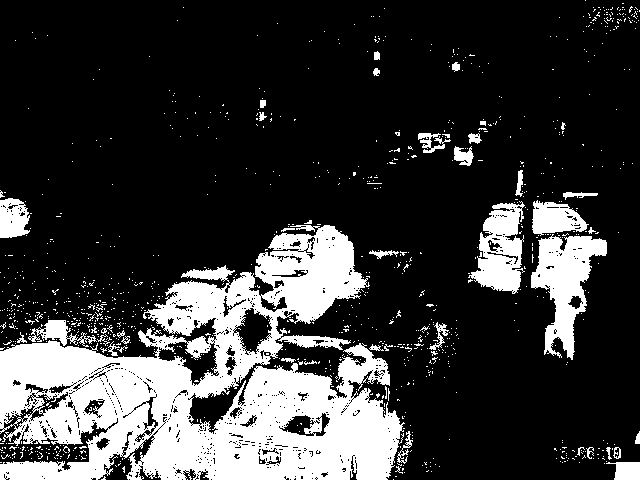
\includegraphics[width=0.48\linewidth, height = 0.3\linewidth]{./img/bg/halsted_FG.png}  
        \subcaption{Ghosting. Vehicles stopped at red light have become part of the background model.} 
        \label{subfig:bg-ghost}
    \end{minipage}
    %\vspace{-0.5em}
    \caption{Common background subtraction failure cases. Pixel values change for many reasons other than motion.}
    \label{fig:tracker-bg}
\end{figure}

In summary, background subtraction provides the ability to capture small movements without manual setup beforehand. However, it is error-prone and must be compensated by other methods to create a robust vehicle tracking system. 

%-------------------------------------------------------------------------
\subsection{Object detection}
\label{subsection:detector}

Object detectors \cite{felzenszwalb2010cascade,girshick2014rich} %viola2001rapid, dalal2005histograms
work on individual frames, scanning the image for areas that appear similar to offline training samples. 
Compared to background subtraction, object detection method tends to be more robust to illumination change and occlusion.
However, the cost of object detection is remarkable, as it often involves an exhaustive search throughout the image, both in location and object size.
%
%The detector usually works as a classifier after offline training, applied exhaustively on every possible window with different scales and ratios across the image. 
%The computation cost comes from the huge number of windows to check.
%Before the boosting of deep neural network, researchers were working on developing representative features.
Cascaded classifiers partially address this by discarding background regions \cite{felzenszwalb2010cascade}.
%Recently, with the development of GPU power and deep neural network architecture, both the feature and representation are greatly improved. 
%The state-of-the-art detector, called faster-RCNN \cite{renNIPS15fasterrcnn}, is used by our system. It integrates scan window filtering during forward passing. The time required for detection on one image drops from 2 seconds \cite{felzenszwalb2010cascade} to 198 ms on the PASCAL 2007 dataset, making real-time detection on videos possible.
More recently, deep neural networks \cite{girshick2014rich,renNIPS15fasterrcnn} have emerged as a promising approach to object detection. %he2014spatial, 
We use a state-of-the-art detector called faster-RCNN \cite{renNIPS15fasterrcnn}.
Running on a high-end graphics processing unit (GPU), the time required for detection on one image drops from 2 seconds \cite{felzenszwalb2010cascade} to 198 ms on the PASCAL 2007 dataset, making the real-time detection in video feasible. 
%It reduces detection time from 2 seconds \cite{felzenszwalb2010cascade} to 198 ms on the PASCAL 2007 dataset, making real-time detection on videos possible. 
However, like other detectors, faster-RCNN still has missing and false detections. In our measurements, it has a missing rate in excess of $65\%$ and $86\%$ on high- and low-resolution videos, respectively.
Thus, given the high miss rate, especially on poor quality images, object detection alone is not suffice for a robust vehicle tracking system. 

%\ref{fig:det_update} gives the number of total detection boxes and ground truth on videos with different resolutions. The detector misses a large number of objects, especially on low resolution videos. 
%This is because tiny vehicles in low resolution videos carry insufficient information for detector. 


% \textcolor{red}{not sure where to put this}such as Haar-like feature \cite{papageorgiou1998general} and HOG feature \cite{dalal2005histograms}.

%On the other hand, although more vehicles are detected on high resolution videos, only about $60\%$ detection boxes are used for tracking update. This indicates that the detector is not always stable and may have false detections.
% \begin{figure}[!htbp]
% \begin{center}
%   \includegraphics[width=\linewidth]{./img/track_detection_update_by_group.pdf}
% \end{center}
%    \caption{Detection count used during tracking.}
% \label{fig:det_update}
% \end{figure}
%-------------------------------------------------------------------------
\subsection{Optical flow}

Optical flow is an estimate of the movement of pixels between two images: in our case, two consecutive video frames. Optical flow provides a low-level description of motion in images and can offer useful evidence for tracking applications.
Estimating optical flow is a research area in its own right,
%\cite{zach2007duality, werlberger2009anisotropic, weinzaepfel2013deepflow}, but as many researchers before us, 
but we use the seminal Lucas-Kanade algorithm \cite{lucas1981iterative} in our system, as it runs fast on GPUs, and provides useful results while making minimal assumptions about the underlying scene and image. 
% in tasks like action detection or activity recognition. We use it to provide motion information besides appearance.
%The basic assumption of optical flow is brightness constancy constraints. 
% However, there is a common problem called \emph{aperture problem}, the local information is not sufficient to infer the global motion, since it is computed on a small neighborhood area. 
%To overcome this and achieve higher accuracy, smoothness constraints \cite{horn1981determining} and more complex regularization \cite{zach2007duality, werlberger2009anisotropic} is added. 
%According to \cite{weinzaepfel2013deepflow}, the current state-of-the-art optical flow algorithm requires $19\sim2000$ seconds for each pair of images. 
%For efficiency, we use the GPU version of Lucas-Kanade optical flow \cite{lucas1981iterative} in OpenCV \cite{opencv_library}.
\ref{fig:tracker-of} illustrates two optical flow problems that may affect tracking accuracy. The left column shows the direction and magnitude of the optical flow vectors, while the right column is the color code visualization of the optical flow results, with the color wheel at bottom right corner of Figure \ref{subfig:of-occlusion} indicating the corresponding direction. % in HSV color space. Direction corresponds to Hue value of the image, and magnitude corresponds to Value plane.
Figure \ref{subfig:of-aperture} illustrates the so-called aperture problem, where the center of the truck has no reported optical flow, due to its large and uniformly colored surface. %it is not likely to get an accurate movement estimation given such small area.
Figure \ref{subfig:of-occlusion} illustrates the ``turbulent'', error-prone flow that occurs where objects traveling in opposite directions meet.   %Since objects are represented as rectangles in our case, it is easy to include such erroneous flow once such case happens.

\begin{figure}[!htbp]
\centering
    \begin{minipage}{0.96\columnwidth}
        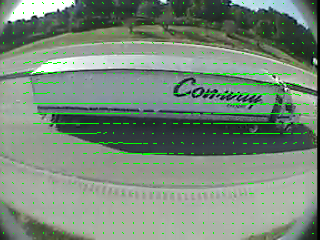
\includegraphics[width=0.48\linewidth, height=0.3\linewidth]{./img/of/252707.png} 
        
\includegraphics[width=0.48\linewidth, height=0.3\linewidth]{./img/of/252707_OF.png}
        \subcaption{Aperture problem.}
        \label{subfig:of-aperture}
    \end{minipage}
    \hspace{0.02\columnwidth}
    \begin{minipage}{0.96\columnwidth}
        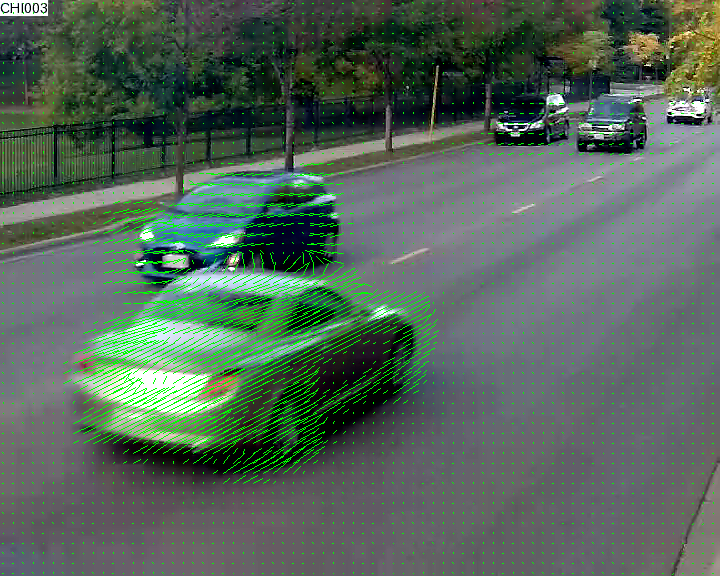
\includegraphics[width=0.48\linewidth, height=0.3\linewidth]{./img/of/ILCHI_CHI003.png}
        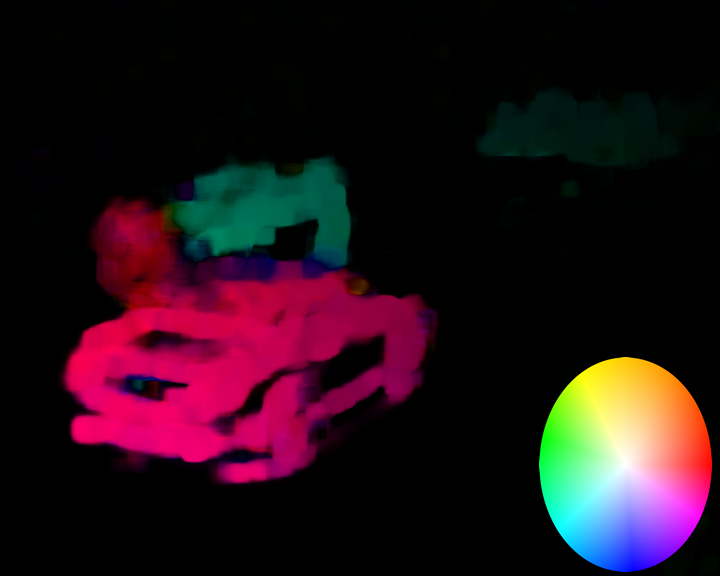
\includegraphics[width=0.48\linewidth, height=0.3\linewidth]{./img/of/ILCHI_CHI003_OF_wheel.png}
        \subcaption{Occlusion ``turbulence''.}
        \label{subfig:of-occlusion}
    \end{minipage}
    % \vspace{-0.5em}
    \caption{Common problems in optical flow estimation.}
    \label{fig:tracker-of}
    % \vspace{-0.5em}
\end{figure}

Thus, while {\it accurate} optical flow estimates offer valuable information about movement in the scene, it is neither complete (due to the aperture problem), nor free of severe estimation errors, in particular near occlusion boundaries. 

\section{Vehicle Tracker by Kalman Filter}
\label{sec:tracker-kf}

\begin{figure}[!htbp]
\begin{center}
    % \vspace{-1em}
    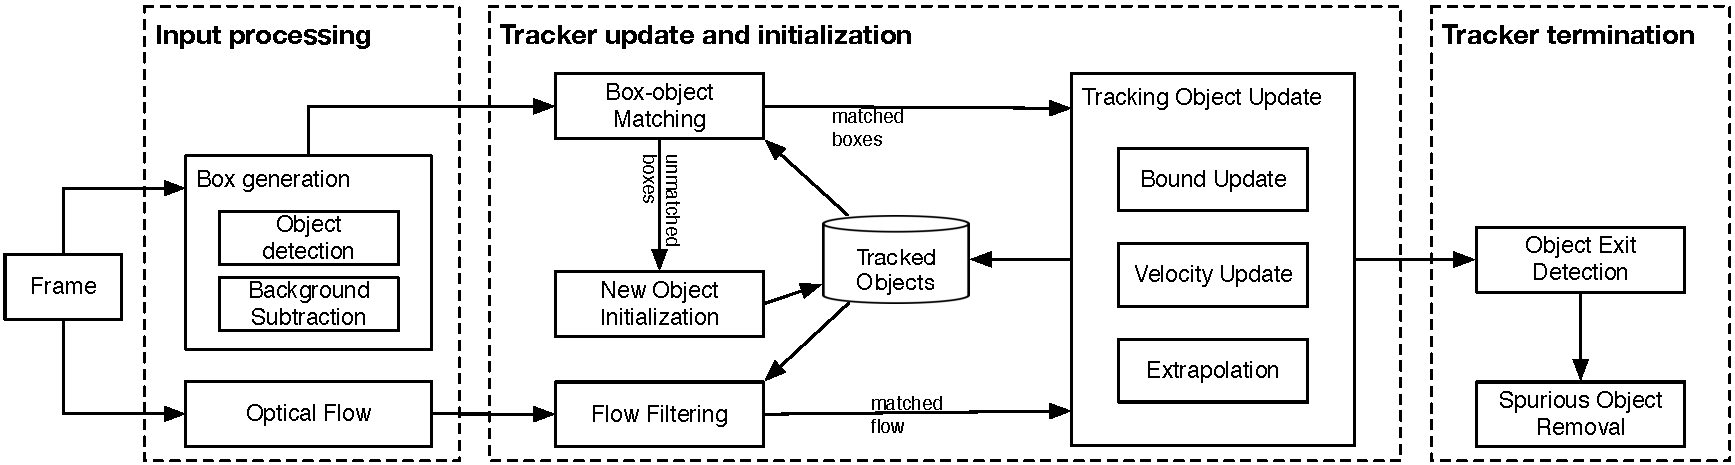
\includegraphics[width=\linewidth]{./img/kalmanFilterTracker.pdf}
\end{center}
    % \vspace{-1em}
   \caption{Overview of proposed system. Separate Kalman filter state is initialized, maintained and terminated for each tracked object. The state is updated based on matching input from background subtraction, object detection and optical flow.}
\label{fig:kf-tracker-workflow}
% \vspace{-1em}
\end{figure}
%We propose an efficient framework based on Kalman Filter, which is jointly updated by background subtraction model, detector and optical flow.
\ref{fig:kf-tracker-workflow} describes the workflow of our automatic tracking application. We first apply background subtraction and object detector on each frame. This generates two sets of candidate boxes, which are used to initialize and update trackers. Each tracker is represented by an individual Kalman filter \cite{grewal2011kalman}. 
Optical flow is also computed. Any flow that matches a tracked object both by location and velocity, is used for tracker update. Tracking is terminated based on object location, velocity and time; short-lived or otherwise spurious objects are filtered out.

\subsection{Model definition}

% \subsection{Kalman filtering for fusing multiple inputs} \label{section:kalmanFilter}

% Given the pros and cons of above methods, we aim to combine them into a single system where the strengths of one method may compensate for the shortcomings of another. For this, we use Kalman filtering, both for its suitability in combining the results of these different methods, and for its ability to compute a smooth estimate from noisy input \cite{grewal2011kalman}. 
% %Kalman filter \cite{grewal2011kalman} is a recursive state estimator of linear dynamic system, with numerous applications in time series analysis, such as navigation, robotic control and signal processing. 

We use Kalman filter to smooth out the noises in the observed measurements by the aforementioned components and more importantly, to integrate the strengths and compensate the weakness of each component. The \emph{prediction} by its linear model is \emph{corrected} with measurements observed over time, therefore the generated estimation is much smoother despite the noises in measurement input. 
%combine the aforementioned unstable components, both for its suitability in combining multiple potentially conflicting measurements into a single coherent model, and for its ability to compute a smooth estimate from noisy input. 
To model the state change, a discrete-time controlled process is modeled as linear stochastic difference equation \cite{Welch:1995:IKF:897831}, state at time $k$ is a linear combination of its previous state $\mathbf{x_{t-1}}$ at time $t-1$
% , a control signal $\mathbf{u}_{k-1}$ 
and the process noise $\mathbf{w}_{t-1}$:
% \setlength{\abovedisplayshortskip}{0pt}
% \setlength{\belowdisplayshortskip}{0pt}
\begin{equation}
  % \mathbf{x}_k = A\mathbf{x}_{k-1} + B\mathbf{u}_{k-1}+\mathbf{w}_{k-1},  
  \mathbf{x}_k = A\mathbf{x}_{t-1} + \mathbf{w}_{t-1}, \label{eq:kf-transition}
\end{equation}
where $A$ is the state transition model.
% , $B$ is a control-input model applied on control vector $\mathbf{u_{k-1}}$. 
In our case, A models how object move on the frame along time, presumably satisfies constant acceleration movement.
There is also measurement $\mathbf{z}\in \mathbb{R}^{m}$ formulated as
\begin{equation}
\mathbf{z}_t = H\mathbf{x}_t+\mathbf{v}_t.
\label{eq:kf-measurement}
\end{equation}
Here $H$ is the measure model, which observation to correct prediction from previous step. $\mathbf{w}_t$ in \ref{eq:kf-transition} and $\mathbf{v}_t$ in \ref{eq:kf-measurement} are process and measurement noise respectively. They are assumed independent of each other and zero-mean Gaussian, with $Q$ and $R$ as process noise covariance and measurement noise covariance, respectively.
\begin{align}
p(\mathbf{w})\sim \mathcal{N}(0, Q)\\
p(\mathbf{v})\sim \mathcal{N}(0, R)
\end{align}
The recursive process of Kalman filter contains two steps: time update (prediction) and measurement update (correction). Both steps are applied at time $k$, indicated by subscripts below.
For such a continuous system, we define a time unit $dt$, which is the time interval we perform an update, in our case, the time between two consecutive frames. Each variable has its own value at a certain time step $t$, indicated by the subscript. The prediction is performed as follows: 
% \setlength{\abovedisplayskip}{2pt}
% \setlength{\belowdisplayskip}{2pt}
% \noindent\textbf{Prediction:}
\begin{align}
\mathbf{\hat{x}}^{\mhyphen}_t & = A\mathbf{\hat{x}}_{t-1} \label{eq:linear-model} \\%+ B\mathbf{u_{k-1}} \label{eq:predictState}\\
P^\mhyphen_t & = AP_{t-1}A^T + Q \label{eq:predict_noisecov_pre}
\end{align}

Here $\mathbf{\hat{x}}_{t-1}$ and $\mathbf{\hat{x}}^{\mhyphen}_t$ are internal states before and after prediction at time $t$. $P_{t-1}$ and $P^\mhyphen_t$ are prior and post error covariances, and $Q$ is the process noise covariance. In our case, we define 
% Here $A$ is the linear transition model to describe the state change over time.
% Each tracked object has a Kalman filter and we have 
the internal state a 10-dimensional vector: $$\mathbf{x}=[x, y, w, h, x', y', w', h', x'', y''],$$ corresponding to the object's top left location $(x, y)$, size $(w, h)$, as well as the velocity ($x',y'$), rate of growth ($w',h'$) and acceleration $(x'', y''$), respectively.
The dynamic model $A$ is defined based on the physics equation of displacement with velocity and acceleration. With the assumption that the object has constant acceleration within $dt$, we have:
% \setlength{\abovedisplayskip}{2pt}
% \setlength{\belowdisplayskip}{2pt}
\begin{align}
  x_t & = x_{t-1} + x'_{t-1}\cdot dt+\tfrac{1}{2}\cdot x''_{t-1}\cdot dt^2 \label{eq:x}\\
  y_t & = y_{t-1} + y'_{t-1}\cdot dt+\tfrac{1}{2}\cdot y''_{t-1}\cdot dt^2 \label{eq:y}\\
  x'_t & = x'_{t-1} + x''_{t-1}\cdot dt \label{eq:xp}\\
  y'_t & = y'_{t-1} + y''_{t-1}\cdot dt \label{eq:yp}.
\end{align}

For width and height, we instead assume constant growth rate within $dt$, thus
\begin{align}
  w_t & = w_{t-1} + w'_{t-1}\cdot dt \label{eq:w}\\
  h_t & = h_{t-1} + h'_{t-1}\cdot dt \label{eq:h}
\end{align} 

% . In our case, we use a constant acceleration movement model; $B$ is a control-input model, but not used here. $H$ is a measurement model, mapping measurements to the states in $\mathbf{\hat x}$. Finally, $Q$ and $R$ are process noise covariance and measurement noise covariance, respectively.

% Thus, $A$ and $Q$ describe feasible object movements, $H$ can accommodate any number of measurements, and $R$ incorporates the expected error in each measurement, as well as correlations between measurements. Below, we describe our proposed system, consisting of central per-object Kalman filter, with detection, background subtraction and optical flow as input. 

% In the prediction step, preliminary prediction of state $\mathbf{\hat{x}^{\mhyphen}}$ and process noise covariance $P^\mhyphen_k$ is made based on value at previous time step. In measurement update step, Kalman gain $K_k$ is first computed and used to correct state estimation $\mathbf{\hat{x}_k}$ and process noise covariance $P_k$. Note that the Kalman gain $K_k$ indicates how much the measurement $\mathbf{z_k}$ is trusted to update the estimation ((\ref{eq:correct})). We update our model with different measurements confidence, by manipulating the measurement noise covariance $R$, in order to have desirable $K_k$. See \cite{Welch:1995:IKF:897831} for more details about Kalman filtering.

% \textbf{Correction:}
After prediction, the estimated state $\mathbf{\hat{x}^{\mhyphen}_t}$ is corrected by an observed measurement $\mathbf{z}$ at each time step by the steps below: 
\begin{align}
K_t & = P^{\mhyphen}_t H^T(HP^{\mhyphen}_t H^T+R)^{-1} \label{eq:predict_gain}\\
\mathbf{\hat{x}_t} & = \mathbf{\hat{x}^{\mhyphen}_t} + K_t(\mathbf{z_t} - H\mathbf{\hat{x}^{\mhyphen}_t)} \label{eq:correct} \\
P_t & = (I-K_tH)P^{\mhyphen}_t \label{eq:predict_noise_cov_post}
\end{align}

In our case, we have a 10-dimensional measurement vector: 
$$\mathbf{z}=[x^{bg}, y^{bg}, w^{bg}, h^{bg}, x^{det}, y^{det}, w^{det}, h^{det}, v_x, v_y],$$ 
which represents the top left coordinates $(x, y)$, width $(w)$, height $(h)$, reported by background subtraction $bg$ and detector $det$, separately, as well as the velocity $(v_x, v_y)$ reported by optical flow estimation. 
The measurement model $H$ is a 10-by-10 matrix of zeros except for ones at $(0, 0),$ $(1, 1),$ $(2, 2),$ $(3, 3),$ $(0, 4),$ $(1, 5),$ $(2, 6),$ $(3, 7),$ $(4, 8),$ $(5,9)$, signifying that the background and detector boxes directly measure $x$, $y$, $w$, and $h$, and that optical flow directly measures $x'$ and $y'$. In other words, there are no direct measurements of $w'$, $h'$, $x''$ or $y''$ since they are not observable.
$R$ is the measurement noise covariance, indicating the noisiness of measurement. By manipulating the measurement noise covariance $R$, we compute a Kalman gain $K_t$, indicating the weight of the measurement to update the corresponding prediction. 
%Finally, $Q$ and $R$ are set based on the observed statistics of each variable (based on our ground truth data). 


\subsection{Measurement acquisition}

%We define the object location $(x, y)$, size $(w, h)$ and velocity $(u, v)$ as our measurement to update the internal states. 
%This section below describes how we generate less noisy measurement values from fallible background subtraction model, detector and optical flow.
None of our input measurements: background subtraction, object detection and optical flow, correspond directly to a single tracked object. Instead, they generate boxes and flow indications for an entire frame.
To produce input to an individual tracked object's filter, we first compute a matching of input data to tracked objects, then apply the matched boxes and flow to the corresponding object's Kalman filter state. 

\textbf{Background subtraction and object detection:}
Both background subtraction and object detection generate bounding boxes $\{x,y,w,h\}$. We only take those consistent with tracker's current state as the measurement. For each Kalman filter, the best matching box as measurement maximizes the total overlap between the predicted bounds of internal filter, and the bounds of the measured boxes. Boxes must overlap with the predicted state in order to be considered a match. Any remaining boxes are used to initialize new tracked objects. 

\textbf{Optical flow:}  
%Figure \ref{fig:flowFilter} shows the process of optical flow filtering.
Optical flow reports velocity on a pixel-by-pixel basis, with many erroneous flow vectors due to the aperture and turbulence problems described earlier. To produce a velocity measurement from the optical flow field for a single object, we first denoise the flow field by forward-backward error thresholding, as described in \cite{kalal2010forward}. We then filter the flow by location, velocity magnitude and direction. In particular, we only consider flow vectors that originate from the location of the object in the previous frame, follow the similar direction (within in $45^\circ$) of the previous state -- to reduce the effect of turbulence problem, and only keep those vectors that fall within twice the error covariance 
(available in $P$, diagonal entries corresponding to the object velocity in $\mathbf{\hat x}$), using the simplifying assumption that flow errors follow a normal distribution. 
%
%Note that these operations are efficiently done on frame level and shared among all objects. When flow vectors are used to compute displacement of single object, we make use of the internal states to help flow filtering. The internal state $(v^x, v^y)$ is the direction of the object computed accumulatively over previous time steps, which indicates the rough direction of the flow. We discard flows that differ with internal state $(v^x, v^y)$ in direction and magnitude, which is especially useful when occlusion happens.
Finally we use the mean of the remaining flow vectors on horizontal and vertical direction, respectively, as the optical flow measurement for the object. 

%% \begin{figure}[!htbp]
%% \begin{center}
%%  \includegraphics[width=\linewidth]{./img/flowFiltering.pdf}
%% \end{center}
%%    \caption{Optical flow filtering.}
%% \label{fig:flowFilter}
%% \end{figure}
\subsection{Model update}

The measurements above are directly plugged into \ref{eq:correct}, however, are of different quality, and oftentimes some of the measurements are missing entirely. For example, the invalid foreground is generated when occlusion happens; detector misses a small-sized object, or aperture problem gives zero movement of object.
We address these problems by varying the measurement noise covariance accordingly, which in turn causes the Kalman filter to choose a gain $K$ that maximizes the quality of the internal state. Recall in \ref{eq:predict_gain}, a large measurement covariance $Q$ would result in a smaller $K$, therefore the measurement weights less in correction. When a measurement is missing, we use the value already in $\mathbf{\hat x}$ as a proxy, and set the covariance to $\infty$. Consequently, once none of the three measurements is available, the tracker merely relies on the internal prediction, which we call \emph{extrapolation}. The tracker could still generate tracking results by the internal linear model during extrapolation. The other two cases in \ref{fig:kf-tracker-workflow} are when at least one bounding box is available (bound update) or only optical flow is obtained (velocity update).

We also apply error gating to the background subtraction and object detection measurements. %We assign measurements different weights for update by manipulating the measurement covariance. 
For example, foreground bounding box that is well overlapped with tracked objects (more than $30\%$ overlap) has a higher confidence than those with other bounding boxes around. Similarly, optical flow have a lower confidence with zero value on both directions, since we have no idea whether the object is still or the aperture problem happens.
%A matched measurement box that has insufficient overlap (below 30\%) with the tracker state is treated as missing. 
In addition, as described in \S\ref{sec:tracker-preliminary}, the three measurement types naturally have different error covariances. Although detector has a higher missing rate, the recall is also high. Therefore, measurement from detector has a smaller noise covariance value than those from background model.

%We propose three different kinds of update mechanisms: bound update, flow update and extrapolation, as shown in Figure \ref{fig:workflow}.
%Bound update is only used when the box is of high confidence, usually applied to moving objects without any occlusion; flow update is when we are not sure about the box, but we have relatively confident optical flow vector, this happens when occlusion or background crashes with illumination change. When neither box nor optical flow is reliable, we hold the state and only predict without correction, this is called extrapolation. Common case is that tracked object is partially occluded or noise. Each update is executed with different measurement covariance based on the certainty of the box and flow vector. 
%Recall that in section \ref{section:kalmanFilter} we mentioned that by tuning measurement covariance $R$, we are able to change the weight (Kalman gain $K_k$ in (\ref{eq:predict_gain})) of measurement in correction step. More specifically, when we update with both bounds and optical flow vector, we make measurement covariance $Q$ small for the location $(x, y, w, h)$ and velocity $(u, v)$, resulting a large $K_k$; if we use flow update, only entries of $Q$ corresponding to velocity $(u, v)$ are given a small value. When in extrapolation mode, measurement covariance matrix will be set a high value, indicating the measurements for neither location nor velocity are certain.
% \begin{table}[!htbp]
% \footnotesize
% \centering
% \caption{Kalman filter update schemes.}
% \begin{tabular}{|m{0.16\linewidth}|m{0.22\linewidth}|m{0.22\linewidth}|m{0.2\linewidth}|}
%   \hline
%       ~   & \textbf{Update condition} & \textbf{Operation}& \textbf{Example case}  \\ \hline  
%   Bound update    &   High confidence in both box and velocity.   & Small $Q$ value for $(x, y, w, h , u, v)$. & Single object without occlusion.\\ \hline
%   Flow update         & Low confidence in box, high confidence in velocity. &  Large $Q$ value for $(x, y, w, h)$, small value for $(u, v)$. & Background model failure or miss detection.\\ \hline
%   Extrapolation       & Low confidence in both box and velocity. &  Large $Q$ value for $(x, y, w, h , u, v)$. & Occlusion or noise.\\ \hline
% \end{tabular}
% \label{table:udpate}
% \end{table}
\section{Fully Automatic Initialization and Termination}
\label{sec:tracker-init-term}
% Tracker initialization is challenging in the vehicle tracker setting. Objects enter and exit the scene in a variety of ways: approach from a distance, enter from the image boundary, appear from behind an occluding object --- moving or stationary, and become visible due to changes in lighting or background conditions. Termination has similar challenges --- vehicles may disappear temporarily behind obstructions or due to changing conditions, they may linger near the edge of the screen, exit the scene while behind a moving vehicle, or disappear slowly into the distance. 

% Many tracking methods in the literature initialization and termination heuristically by manually labeling an entry/exit area beforehand, under the assumption that objects always enter or exit within a certain area, or rely on fully manual initialization. The first method is too simplistic for general purpose vehicle tracking, and the second is impractical. 
\subsection{Object entry and exit} 
\label{subsec:tracker-entry-exit}

Currently available datasets usually have tracked objects in the center of the first frame, however, we have initialization more challenging when objects enter the scene in a variety of ways: approach from a distance, enter from the image boundary, appear from behind an occluding object --- moving or stationary, and become visible due to changes in lighting or background conditions. Termination has similar challenges --- vehicles may disappear temporarily behind obstructions or due to changing conditions, they may linger near the edge of the screen, exit the scene while behind a moving vehicle, or disappear slowly into the distance. It is usually natural to terminate tracking when sequence ends or object leaves the scene in short sequences, whereas in practice, it is hard to distinguish between exiting and temporal occlusion when the object is not visible in long-time videos.

As automatic initialization and termination are missing in the majority of current tracking literature, the generally accepted methods either heuristically manually label an entry/exit area beforehand, under the assumption that objects always enter or exit within a certain area, or rely on fully manual initialization. The first method is too simplistic for general purpose vehicle tracking, and the second is impractical under constrained expense/time budget for large-scale use.

%By analyzing our currently available videos across our state from local transportation department, despite the various size changing patterns while objects move in the scene, in most cases, they are composed by two basic cases: expanding and shrinking. With size changing, initialization with incomplete or insufficient appearance would easily result in tracking failure, which is common when object size is expanding; on the other hand, late initialization would result in a short trajectory. Usually surveillance tasks require complete and accurate movement monitoring from video, balance of tracking performance and object lifetime is a necessary problem to consider.

In the only available literature that explicitly addresses the effect of tracker initialization \cite{Wu_2013_CVPR}, the author concludes that slight temporal and spatial variation would result in performance difference. 
However, unlike the currently available dataset, vehicles frequently encounter significant scale change while leaving or entering the scene in the traffic surveillance videos available to us. This presents a unique problem for initialization, as early initialization would result in a small, poor-quality image, and late initialization results in missing of information due to the short trajectory. Thus, striking the right balance between tracking performance and lifetime is the key to automatic tracker initialization.

% \begin{figure}[!htbp]
% \centering
%     \begin{minipage}{0.48\columnwidth}
%         \includegraphics[width=\linewidth, height=0.6\linewidth]{./img/init_thresh1.pdf} 
%         \subcaption{Size expanding.}
%         \label{subfig:sh}
%     \end{minipage}%
%     \begin{minipage}{0.48\columnwidth}
%         \includegraphics[width=\linewidth, height=0.6\linewidth]{./img/init_thresh2.pdf}
%         \subcaption{Size shrinking.}
%         \label{subfig:shrink}
%     \end{minipage}%
%     \caption{Object movement model. Two basic cases for object entry and exiting. Number under arrow shows the size ratio with respect to the largest size along the sequence. Frame in gray indicates the first frame with a size ratio larger than 0.6.}
%     \label{fig:entryExist}
% \end{figure}

\subsection{Our Method}
Our system initializes new trackers based on unmatched boxes from background subtraction and object detection. This supports the challenging cases described above, but can result in many spurious trackers due to the noisy nature of both background subtraction and optical flow. We use a two-pronged approach to limit such spurious results. First, initialization is limited to objects larger than 10$\times$10 pixels. This reduces the number of trackers in flight, without significant negative effect: 
cars that could reasonably be captured tend to be larger than that in our videos, except when approaching from or driving toward the vanishing point. 
% we do not need to start tracking when the object is near the vanishing point, but can do so when the object becomes reasonably large.
Second, trackers are terminated when the object leaves the frame, after no direct observations (boxes or optical flow) has been made for 50 frames, in other words, in \emph{extrapolation} mode. Any object would have such 50 frames before exit. However, upon termination, tracked objects are validated based on the number of observations and distance traveled. Spurious noise tends to be stationary and short-lived, whereas vehicles typically follow a continuous and long-lived path through the scene. To adapt to the variety of videos and objects, distance threshold is dynamically computed by object size and video resolution. 
%During the extrapolation of uncertainty for 50 frames, the Kalman filter could still make predictions by the internal state. 
One good consequence of such scheme is that many early initialized noises are quickly discarded, since usually there is no consistent measurement available for them, while those tiny objects discarded as noises are soon available for future initialization, with better quality. Therefore, real small objects are able to be initialized at the earliest point and survive with a complete trajectory. 

%Initialization and termination has to happen at a right moment. We have to handle the transitional stage where the object is partially visible, when objects enter/exit near frame boundary. We also have to decide whether the box is sufficiently reliable if it is too small. Early initialization may result in partially tracked or drifted objects, while late termination would force the tracker to track background, or even worse, other object around.

%In our system, we initialize trackers as early as possible, except those tiny ones. 
%Termination is executed if after 50 frames of extrapolation. The advantage of it is that it handles noises and all other exit cases. Correctly tracked objects become extrapolation mode after being out of view; while noises are usually hard to have corresponding foreground boxes or detection results consecutively, therefore, very easy to fall in extrapolation mode. Only objects move long distance in a sufficiently long lifetime would exited normally, otherwise they are removed as noises. In this way, we generate long trajectory while discarding noisy objects.


% \textbf{Initialization:} For the first scenario, we have to handle the transitional stage where the object is partially visible. The moment of full entering has to be identified, in order to initialize the tracker with complete object appearance. In the second case, the tiny size carries insufficient information for accurate tracking, tracker initialized at such stage is prone to drift. As for the the last scenario, if the entry area is manually setup, the object may be missed since it becomes visible until being outside the entry area. 

% \textbf{Termination:} Early termination may make the object available for initialization since it is still visible. Late termination forces trackers to keep tracking, possibly background, or even worse, another object nearby. This is common in the last two scenarios.

% In conclusion, initialization and termination has to happen at a right moment. Trackers should begin early and terminate late to cover the object's lifetime as long as possible. However, initialization should begin with sufficient information to make sure of the tracking accuracy, while termination should be performed properly in time.
% In our system, we initialize trackers as early as possible, except those tiny ones. 
% Termination is executed if after 50 frames of extrapolation. The advantage of it is that it handles noises and all other exit cases. Correctly tracked objects become extrapolation mode after being out of view; while noises are usually hard to have corresponding foreground boxes or detection results consecutively, therefore, very easy to fall in extrapolation mode. Only objects move long distance in a sufficiently long lifetime would exited normally, otherwise they are removed as noises. In this way, we generate long trajectory while discarding noisy objects.

%-------------------------------------------------------------------------
\section{Evaluation} 
\label{sec:tracker-eval}

\subsection{Tracker configuration}

To better evaluate how each component contributes to the tracker in videos under various conditions, we use three different configurations of our tracking system, based on the inputs used. BG uses background subtraction and optical flow, DET uses the object detector and optical flow, and BG+DET uses all three inputs. 
We also run several state-of-the-art trackers, including KCF \cite{henriques2015high}, STRUCK \cite{hare2011struck}, ASMS \cite{vojir2014robust}, DAT\cite{possegger2015defense}, staple \cite{bertinetto2016staple}, MEEM \cite{zhang2014meem} and SRDCF \cite{danelljan2015learning} as baselines. 
%STRUCK is the top-scorer on a variety of videos a recent (2015) benchmark paper \cite{wu2015object}. 
Since all these trackers require manual initialization (namely human input), they are not able to be compared with our tracker directly. Instead, we can only partially evaluate them by providing manual initialization, see \S\ref{subsec:tracker-eval-overall}. By carefully selected manual initialization, the comparison here is in favor of the baselines.

%-------------------------------------------------------------------------
\subsection{Evaluation metrics}

Given a set of generated and ground truth object trajectories, usually represented by a sequence of rectangular bounding boxes, we desire one or more performance metrics that capture the accuracy of the proposed system. Aspects that need to be captured include 1) tracking duration---if a ground truth trajectory of an object contains N frames, for how many of these frames does the system track the object, 2) recall---how many of the ground truth trajectories were represented in the tracking result, 3) precision---what proportion of tracking results had a corresponding trajectory, as well as 4) the overlap between the tracking result and the ground-truth.

Note that our problem does not fit into common multi-object tracking setting, since moving objects are tracked individually, instead of being modeled globally. Common metrics such as MOTA \cite{bernardin2008evaluating} generates a meaningless number since we can have potentially more objects tracked than ground truth.

As the first step, we match each ground truth to a tracking result, by maximizing the accumulated overlap ratio $r$, 
\begin{align}
    r=\frac{\sum_t{(S_t^{gt}\cap S_t^{traj})}}{\sum_t{(S_t^{gt}\cup S_t^{traj})}},
    \label{eq:ratio-all}
\end{align}
where $S_t^{gt}$ and $S_t^{traj}$ are ground truth and trajectory box areas at frame $t$, respectively. Note that the sum is computed over the union of trajectory and ground truth lifetime. 
%For example, the ground truth appears from frame 1 to 100, while object tracker lasts from frame 20 to 150, the denominator is summed over frame $1\sim150$. 
%Suppose we have two trajectories overlap with the same ground truth, one tracks well in a short period while the other tracks almost as well, but for a longer duration. 
\ref{eq:ratio-all} ensures the ground truth is matched to a longer trajectory with reasonable coverage. 
Additionally, to filter some spurious objects slightly touched the ground truth, we also require any match to have more than $30\%$ overlap on at least one frame, where the value is set experimentally.

%On the other hand, it is more than a collection of manually initialized single-object trackers. The falsely tracked objects due to automatic initialization should be minimized and one-to-one matching of automatically generated trajectories and ground truth should be made before any accuracy evaluation is performed.
%Several metrics have been proposed in the past, including Fscore \cite{kwon2009tracking}, deviation \cite{sanin2012shadow}, and object tracking accuracy (MOTA) \cite{bernardin2008evaluating}. 

%While these work for pure tracking evaluation, where initialization and termination (usually the end of the video clip) is given, these are not well suited to our dataset. 
\subsection{Object-level evaluation} 
\label{subsec:tracker-eval-count}

Given the matched results, we can calculate the proportion of ground truth trajectories that were matched to the tracking result (recall), and the proportion of tracking results that had a matching trajectory (precision), for our three trackers and two types of videos. 
\ref{fig:kf-eval-count-low} and \ref{fig:kf-eval-count-high} show the results in absolute numbers, also to provide some perspectives on the scale of the evaluation. The true positives are those correctly tracked objects and false positives are noisy objects. Our best tracker configuration, BG+DET, achieves $81\%$ recall and $87\%$ precision on our low resolution, simple videos, and $65\%$ recall, $57\%$ precision on the high-resolution, complex scenes. Here, the majority of failures in the complex scenes were due to complicated interactions and heavy occlusion throughout the scene, where vehicles were only partially visible. Currently, we do not split such merged objects into their constituent parts; we leave this for future work. 

Comparing the three configurations, we see that the detector performs quite poorly on the low-resolution scenes, due to small and poor quality imagery where it is sometimes difficult even for a person to correctly identify an object as a vehicle. By contrast, background subtraction does quite well on these uncomplicated scenes. For the more higher resolution complex scenes, the detector performs well, while the background subtraction model struggles and largely introduces noise.

% \setlength{\belowcaptionskip}{-10pt}
\begin{figure}
  \centering
    % \begin{minipage}{0.45\linewidth}
    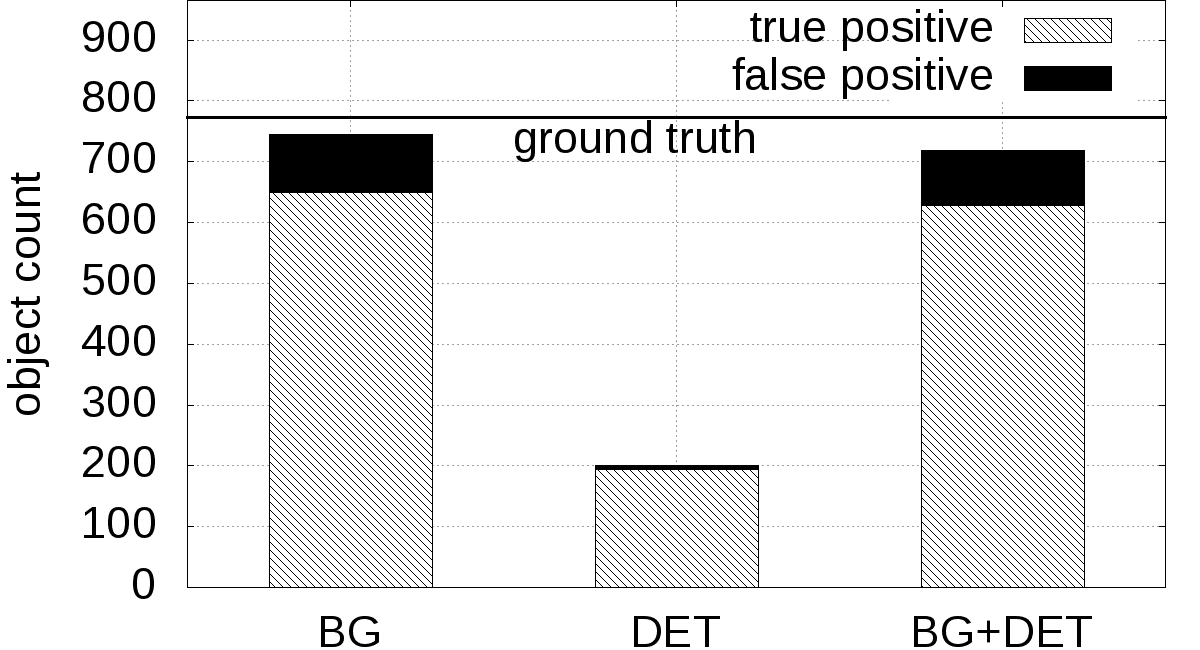
\includegraphics[width=\linewidth]{./img/evaluation/count_lowRes.png}
    \caption{Tracked object count on low resolution, less complex scenes.}
    \label{fig:kf-eval-count-low}
    %\vspace{-0.5em}
    % \end{minipage}
\end{figure}
\begin{figure}
    \centering
    % \begin{minipage}{0.45\linewidth}
    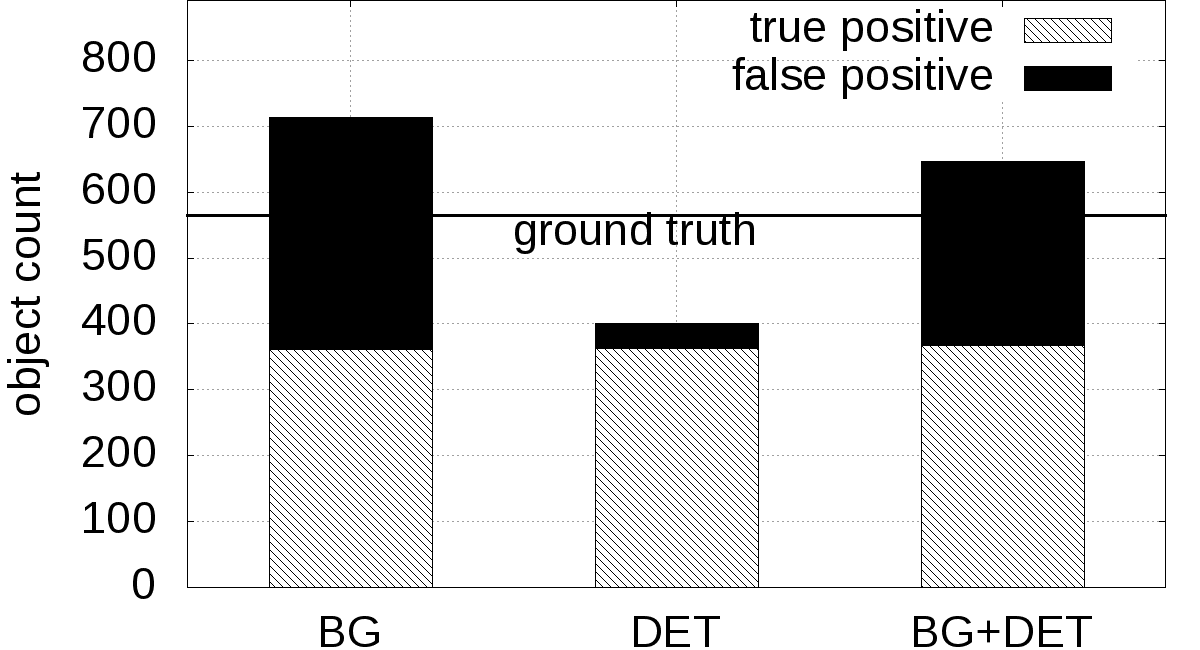
\includegraphics[width=\linewidth]{./img/evaluation/count_highRes.png}
    \caption{Tracked object count on high resolution, more complex scenes.}
    % \end{minipage}
    % \caption{Tracked object count under different tracker settings.}
    \label{fig:kf-eval-count-high}
\end{figure}
%-------------------------------------------------------------------------
% \subsubsection{Overlap area during match}
% \begin{figure*}
% \begin{minipage}{0.33\textwidth}
%   \includegraphics[width=\linewidth]{./img/initOverlap/overlapArea_lowRes.pdf}
%       \subcaption{Simple low resolution videos.}
%   \label{fig:area_lowRes}
% \end{minipage}
% \begin{minipage}{0.33\textwidth}
%   \includegraphics[width=\linewidth]{./img/initOverlap/overlapArea_highRes.pdf}
%       \subcaption{Complex high resolution videos.}
%   \label{fig:area_highRes}
% \end{minipage}
% \begin{minipage}{0.33\textwidth}
%   \includegraphics[width=\linewidth]{./img/initOverlap/overlapArea_night.pdf}
%       \subcaption{Night videos.}
%   \label{fig:area_night}
% \end{minipage}
%   \caption{Mean overlapped area of every object on each frame.}
% \end{figure*}
%-------------------------------------------------------------------------
% \subsubsection{Deviation during match}
% \begin{figure*}
% \begin{minipage}{0.33\textwidth}
%     \includegraphics[width=\linewidth]{./img/initDeviation/deviation_lowRes.pdf}
%     \subcaption{Simple low resolution videos.}
%     \label{fig:deviation_lowRes}
% \end{minipage}
% \begin{minipage}{0.33\textwidth}
%     \includegraphics[width=\linewidth]{./img/initDeviation/deviation_highRes.pdf}
%     \subcaption{Complex high resolution videos.}
%     \label{fig:deviation_highRes}
% \end{minipage}
% \begin{minipage}{0.33\textwidth}
%     \includegraphics[width=\linewidth]{./img/initDeviation/deviation_night.pdf}
%     \subcaption{Night videos.}
%     \label{fig:deviation_night}
% \end{minipage}
%     \caption{Mean center deviation of every object on each frame.}
% \end{figure*}
%-------------------------------------------------------------------------


\subsection{Pixel-level evaluation during entire lifetime} 
\label{subsec:tracker-eval-overall}

We are also interested in evaluating how well the tracker follows objects in the scene. For example, as one of our motivating application, accurate tracking is necessary for correct turning movement classification, as \ref{fig:screenshots}\subref{subfig:193402} illustrates.
While there exists no similar work or benchmark that incorporates automatic initialization, we can only partially compare our system to prior work. Here, we modify our tracker to accept manual initialization. Both our modified trackers and the baseline trackers are initialized with boxes extracted from ground truth. These ``initialized'' trackers are then evaluated along with our automatically initialized trackers. Note that the experiment is designed in favor of those manually initialized trackers, since the initialization boxes are from ground truth and perfectly match the object in the scene.

To accept manual initialization in scenes with significant scale change, each tracker is initialized with the first box of ground truth larger than a threshold: 
\begin{align}
    S_{thresh}=\left[\text{max}(S^{gt})-\text{min}(S^{gt})\right]*s + \text{min}(S^{gt}),
    \label{eq:thresh}
\end{align}
where $\text{max}(S^{gt})$ and $\text{min}(S^{gt})$ are the maximal and minimal ground truth areas along the sequence. $s\in \{0, 0.2, \dots, 1.0\}$, corresponds to the minimum fraction of the maximum object size at which initialization may occur. Note $s$ only affects objects that enter with an increasing size; while shrinking objects can be initialized upon appearance regardless of the threshold. 
Tracking is terminated at the last frame of ground truth. 
% Different with \cite{Wu_2013_CVPR}, we do not do any re-initialization after failure, since we are evaluating one-time tracking.
We arrived at this design as some trackers tend to perform poorly when initialized by small images, yet delaying initialization until the object grows large can result in arbitrarily shortened trajectory.

\ref{fig:kf-eval-overlap-low} and \ref{fig:kf-eval-overlap-high} compare the overlap ratio of our three tracker configurations both with manual and automatic initialization (horizontal lines), as well as the overlap ratio of several other trackers on our high- and low-resolution datasets. 
The x-axis is the initialization threshold $s$ in \ref{eq:thresh}, and the y-axis is the overlap ratio $r$ from \ref{eq:ratio-all}, averaged over all objects.
This is computed from the first to the last frame of ground truth for the manually initialized and terminated trackers. While for our automatic trackers, it is computed over the union of tracking and ground truth lifetimes. This accounts for both tracking accuracy and lifetime, as we illustrated before.

% \setlength{\belowcaptionskip}{-10pt}
\begin{figure}
  \centering
  % \begin{minipage}{0.45\linewidth}
    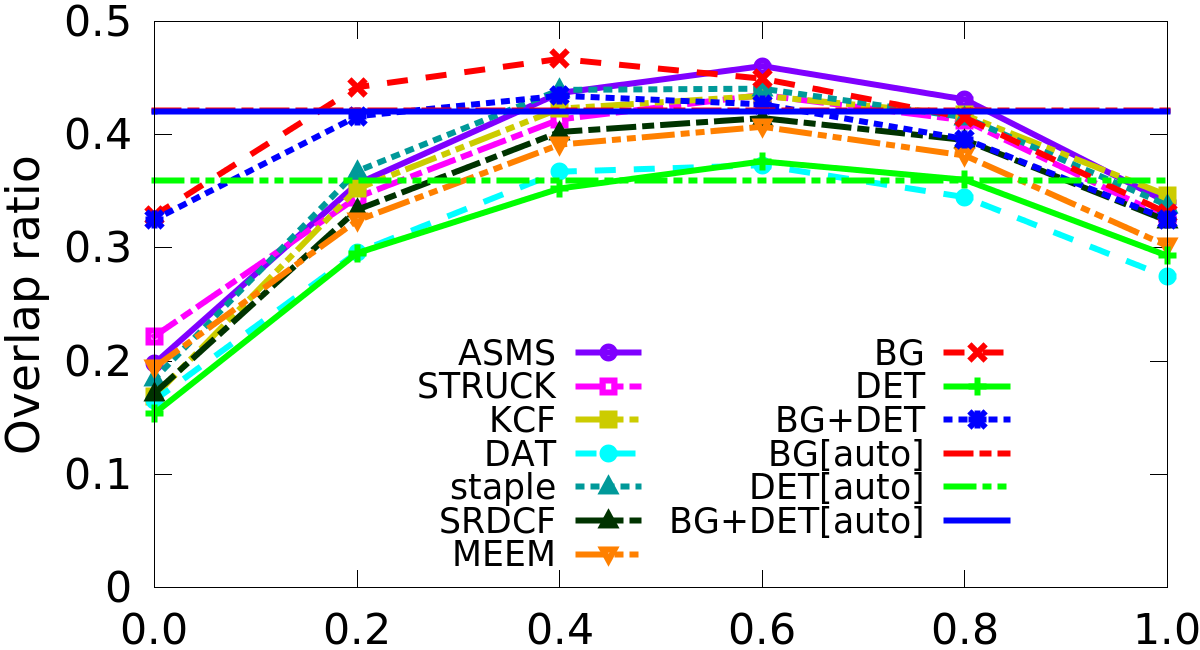
\includegraphics[width=\linewidth]{./img/evaluation/overlapRatioAllPerObj_lowRes.png}
    \caption{Overall overlap ratio on low resolution, less complex scenes.}
    \label{fig:kf-eval-overlap-low}
    %\vspace{-0.5em}
    % \end{minipage}
    % \begin{minipage}{0.45\linewidth}
\end{figure}
\begin{figure}
    \centering
    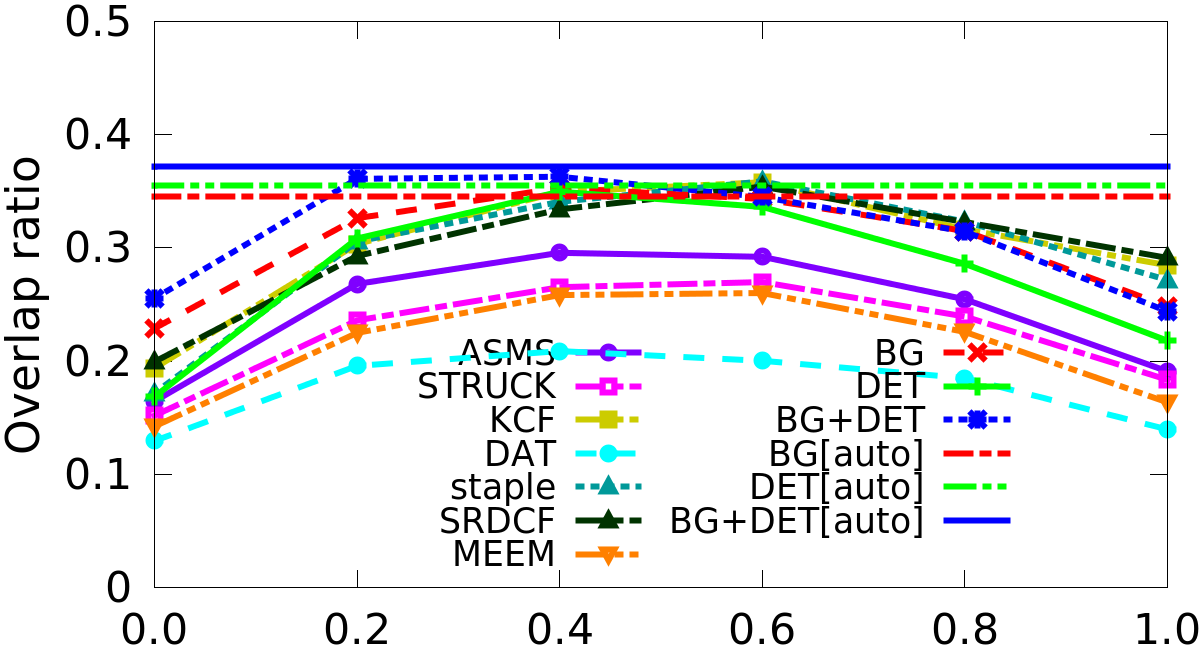
\includegraphics[width=\linewidth]{./img/evaluation/overlapRatioAllPerObj_highRes.png}
    \caption{Overall overlap ratio on high resolution, more complex scenes.}
    % \end{minipage}
    % \caption{Overall overlap ratio.}
    \label{fig:kf-eval-overlap-high}
\end{figure}

The shape of the curves for the initialized trackers captures the trade-off between early-and-inaccurate, vs. late-but-accurate initialization. Overall, our BG-based trackers handily outperform other trackers when manual initialization and termination is provided. More importantly, the auto-initialized BG trackers essentially meet the performance of other trackers on the simple videos, and significantly outperform them on the complex videos. We hypothesize that the automatic initialization allows the tracker to better adapt to individual vehicles vs. the constant threshold set for manual initialization. Additionally, consistent with our conclusion in \S\ref{subsec:tracker-eval-count}, detector dominates the tracking update on high resolution videos, while background subtraction plays its role on low resolution videos.

\subsection{Pixel-level evaluation during tracked period} 
\label{subsec:tracker-eval-acc}

Then we focus on the performance during only the tracked period. Borrowed from standard single object tracking measurement, we show the success plot for trackers for two video groups, in \ref{fig:kf-eval-success-low} and \ref{fig:kf-eval-success-high}. Different from above, we compute the success frame rate from the initialization frame, instead of entire ground truth sequence. The performance is measured by the area under the curve. By \ref{fig:kf-eval-overlap-low} and \ref{fig:kf-eval-overlap-high} we see overlap ratio between 0.2 and 0.6 is a good balance of tracking accuracy and trajectory completeness, we hereby show results of initialization threshold of 0.4 here.
Our automatic trackers significantly outperform other trackers with manual initialization. This demonstrates that proper initialization is critical to the tracking performance and similar conclusion about the contribution of each tracking component can be drawn.

% \setlength{\belowcaptionskip}{-10pt}
\begin{figure}
  \centering
  % \begin{minipage}{0.45\linewidth}
    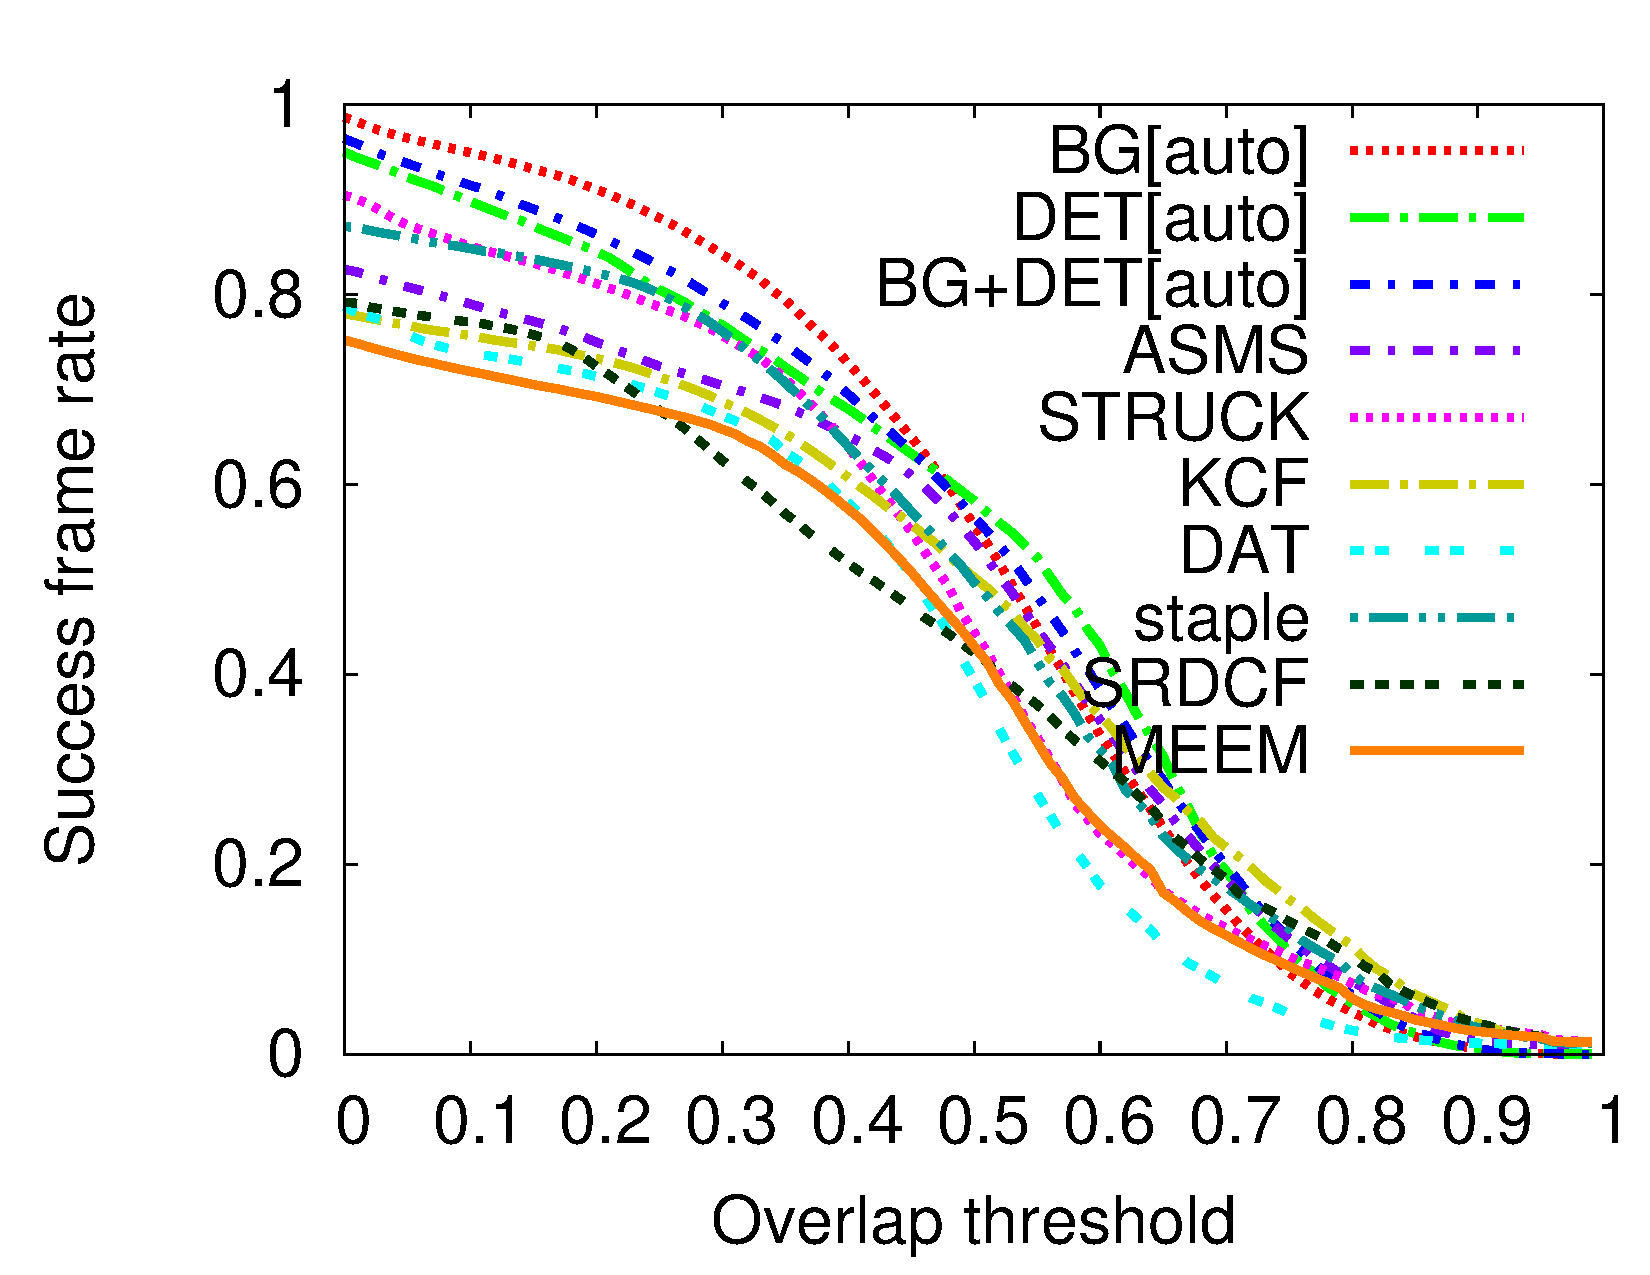
\includegraphics[width=\linewidth]{./img/evaluation/success_lowRes.pdf}
    \caption{Success plot of low resolution, less complex scenes.}
    \label{fig:kf-eval-success-low}
\end{figure}
    %\vspace{-0.5em}
% \end{minipage}
% \begin{minipage}{0.45\linewidth}
\begin{figure}
  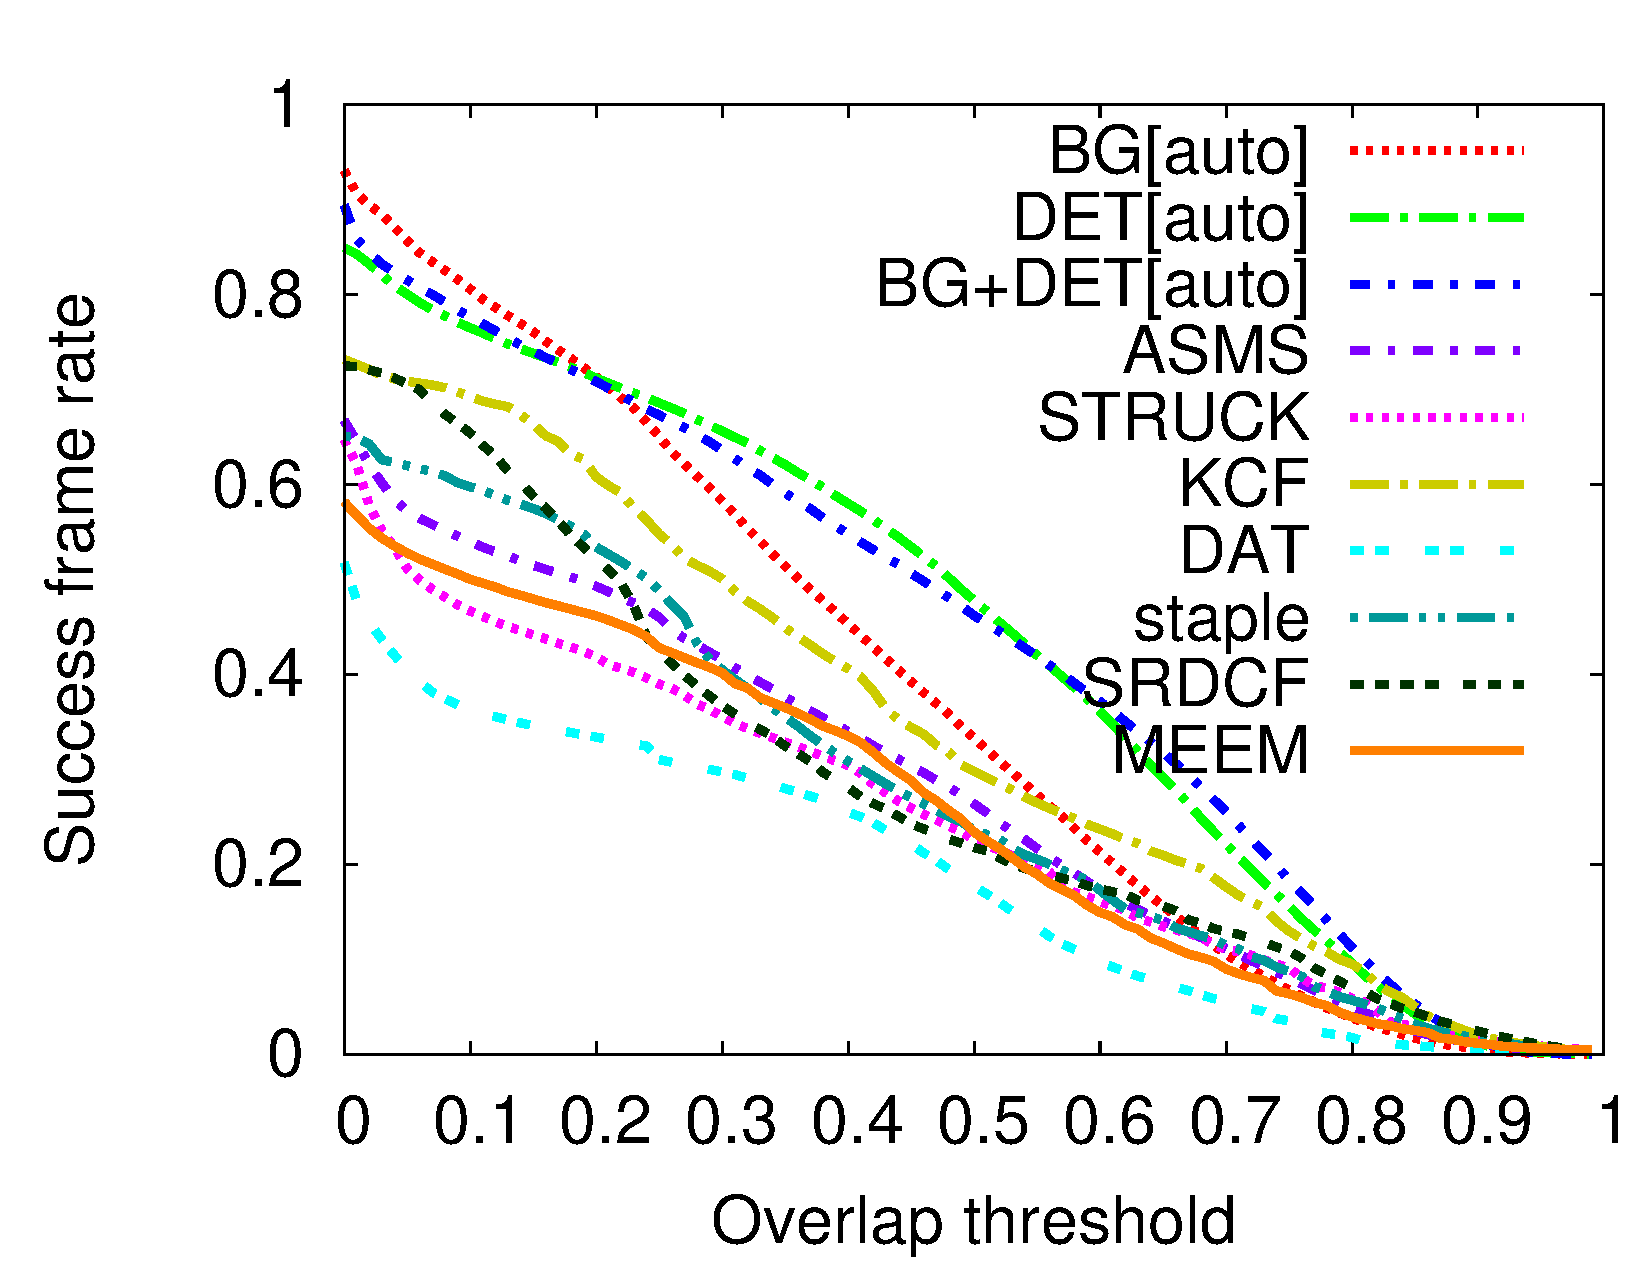
\includegraphics[width=\linewidth]{./img/evaluation/success_highRes.pdf}
    \caption{Success plots of high resolution, more complex scenes.}
% \end{minipage}
  % \caption{Success plots.}
  \label{fig:kf-eval-success-high}
\end{figure}

%% \subsection{Overlap ratio during tracking}\label{subsection:matchRatio}
%% As a supplement, we present the tracking accuracy during the tracking process, thus ignoring the trade-off between duration and accuracy. The only difference compared with the previous subsection is that the overlap ratio $r$ is computed during tracking only: from the initialization frame to last frame of ground truth, instead of from the first frame of ground truth.

%% In Figs \ref{fig:ratio_lowRes}--\ref{fig:ratio_highRes}, the overlap ratio grows with the initialization threshold, then largely levels out rather than drop as in Figs \ref{fig:ratioAll_lowRes}--\ref{fig:ratioAll_highRes}. Thus tracking performance improves with better initialization up to some point. With thresholds of 1.0, a small drop is recorded in some curves---this is likely noise due to the very short tracking duration under that setting. 

%% Consistent with previous results, BG and BG+DET are very similar and the most accurate. Fig \ref{fig:ratioMatch}(\subref{subfig:ratio_lowRes}) shows more similar trend with Fig \ref{fig:ratioAll}, indicating that initialization with small size may affect the tracking accuracy.

%% Based on Fig \ref{fig:ratioMatch} and Fig \ref{fig:ratioAll}, we conclude that $s$ between 0.2--0.6 is a good balance between accuracy and lifetime and our automatic tracker achieves almost the same performance in terms of such balance.
%% \begin{figure}
%%   \centering
%%  \includegraphics[height=1.8in]{./img/initOverlapRatioMatch/overlapRatioMatch_lowRes.pdf}
%%      \caption{Overlap ratio during the tracking process only, on low resolution videos.}
%%  \label{fig:ratio_lowRes}
%% \end{figure}
%% \begin{figure}
%%         \includegraphics[height=1.8in]{./img/initOverlapRatioMatch/overlapRatioMatch_highRes.pdf}
%%      \caption{Overlap ratio during the tracking process only, on high resolution videos.}
%%  \label{fig:ratio_highRes}
%% \end{figure}
\begin{figure}
    \centering
    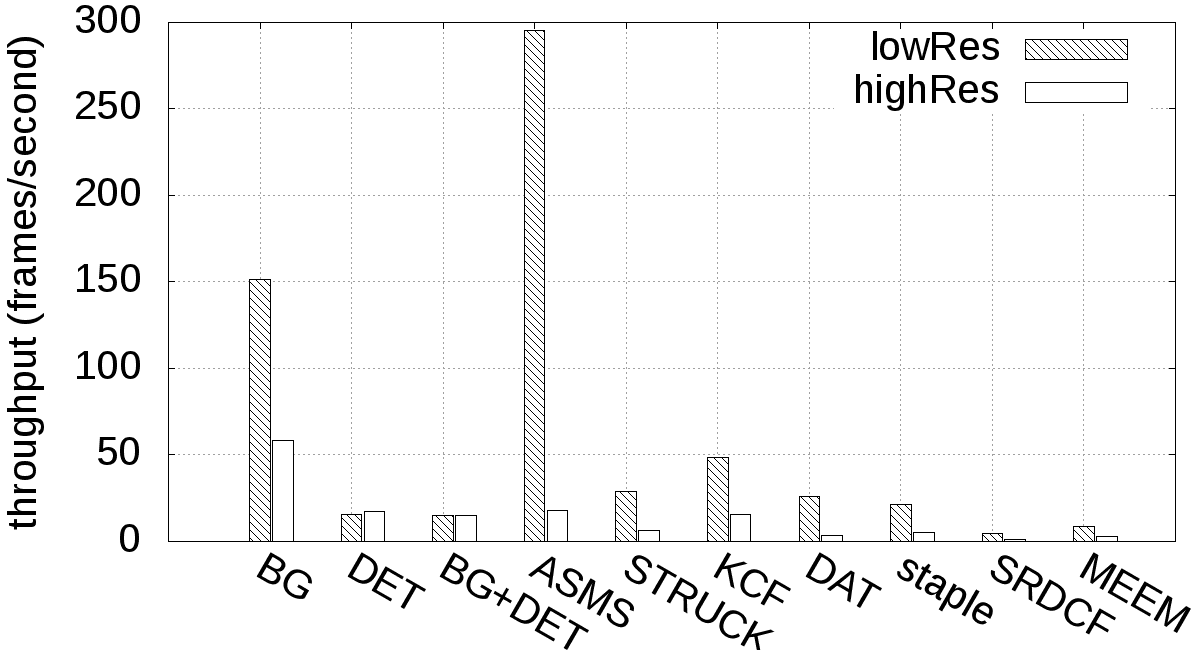
\includegraphics[width=\linewidth]{./img/evaluation/throughputInit_group.png}
   \caption{Tracker throughput on different resolution videos.}
    \label{fig:kf-eval-throughput}
\end{figure}

\subsection{Throughput}
Finally, we explore the throughput of trackers on different resolution videos, as shown in \ref{fig:kf-eval-throughput}.
The evaluation was done on a Linux desktop with an Intel Core i7-3770 3.40GHz processor and a GeForce GTX TITAN X GPU.
According to these results, BG significantly outperforms 6 out of 7 baseline trackers, with around 5$\times$ throughput improvement compared with real time (about 30 fps). Interestingly, ASMS outperforms our BG tracker on low resolution videos, however, it becomes 17$\times$ slower once it is applied on high resolution videos. Although the use of the object detector (DET, BG+DET) makes the tracker slower, they are the only ones that maintain a similar frame rate on both low- and high resolution videos near real time, showing good scalability of resolution.
% it is able to maintain frame rate, with the intermittent detector versions going dramatically faster. 
%The difference between low and high resolution videos becomes negligible when the detection interval decreases. We believe the reason behind this is that the GPU is not fully utilized by the detector on low resolution videos. %Overall BG is more suitable for time-critical application, while DET and BG+DET have high tolerance of resolutions.


%-------------------------------------------------------------------------
\section{Related work}
%-------------------------------------------------------------------------
%Object tracking
\textbf{Object tracking:}
Object tracking algorithms fall into either multi-object or single object tracking category. Multi-object trackers deal primarily with the combinatorial task of associating sets of detections across frames, often modeled as a graph-based global optimization problem 
\cite{butt2013multi,berclaz2011multiple}.
% \cite{zhang2008global,pirsiavash2011globally,henriques2011globally,butt2013multi,berclaz2011multiple}.
%among which a large set of methods try to solve the association globally. 
%Popular methods include linear programming \cite{jiang2007linear}, K-shortest path \cite{berclaz2011multiple}, network flows \cite{zhang2008global,pirsiavash2011globally,henriques2011globally,butt2013multi}, maximum weight independent sets \cite{brendel2011multiobject} and continuous energy minimization \cite{andriyenko2011multi}. 
Such methods are computationally expensive, and typically impractical in time-critical applications. Meanwhile, single object tracking has experienced a rapid progress with the help of robust feature representation \cite{kwon2010visual} %jepson2003robust 
and better learning scheme such as SVM \cite{hare2011struck} and boosting \cite{grabner2006real}. 
%,grabner2008semi}, multiple instance learning \cite{babenko2009visual}.
%The generative models look for the most similar objects, with more robust and adaptive appearance models \cite{jepson2003robust,kwon2010visual}. On the other hand, discriminative models are proven to be superior. Various classifiers are trained to separate the object and the background, such as SVM \cite{hare2011struck,bai2012robust}, boosting \cite{grabner2006real,grabner2008semi}, multiple instance learning \cite{babenko2009visual}. Recently correlation filter \cite{henriques2015high} has proven to be the state-of-the-art in terms of performance and speed.
However, object tracking still remains a challenging problem due to the difficulty caused by changing appearance and occlusions. To cope with appearance change, better affinity measurement \cite{choi2015near} and adaptive learning schemes \cite{kalal2012tracking} may help.
For occluded objects, multi-object trackers tend to inherently model occlusion, for example, using augmented graph representation \cite{butt2013multi} %, pirsiavash2011globally,henriques2011globally}; 
%In multi-object tracker, \cite{perera2006multi} tries to keep object identity during detection linking, \cite{butt2013multi, pirsiavash2011globally} assumes some object may be invisible for a while and allows link between non-consecutive frames in a network flow graph, \cite{henriques2011globally} explicitly defines an augmented graph to include merge and split. 
while single object trackers maintain the memory of the object appearance \cite{kalal2012tracking}.
% Additionally, we see such generally designed algorithms may have restricted applicability on particular videos. For example, TLD tracker \cite{kalal2012tracking} handles long-time occlusions due to its memory, but may switch to similar object when the target is invisible. On the contrary, \cite{zhang2013structure} is good at discriminating similar objects, only when tracked objects maintain the relative location. 
%As a result, video-specific features are applied for specific tasks such as crowd tracking \cite{zhao2012tracking,zhou2012understanding} and non-rigid object tracking \cite{godec2013hough, duffner2013pixeltrack}.
%trackers are proposed correspondingly. Crowd tracking usually has very tiny objects of interest, therefore motion patterns are widely used \cite{zhao2012tracking,zhou2012understanding}; for non-rigid object tracking, segmentation is introduced to extract accurate object representation \cite{godec2013hough, duffner2013pixeltrack}.
%In this paper, we focus on traffic videos with rigid objects of similar appearance and recurrent motion patterns. 

%-------------------------------------------------------------------------
%Object initialization
\textbf{Tracker initialization and termination:}
Trackers today are evaluated in an idealized setting, where manual initialization and termination is provided.
Most multi-object trackers assume excellent detector performance, but do handle object entry/exit. They either model it intrinsically by adding entry/exit nodes to the optimization graph
\cite{zhang2008global}, 
%,henriques2011globally,pirsiavash2011globally,zamir2012gmcp} 
or manually by defining an entry and exit area
\cite{andriyenko2011multi}.
%,berclaz2011multiple,zhou2012understanding}. 
%In single object tracking evaluation, trackers typically are provided with a manually cropped box on the first frame and terminate at the last frame, assuming that object appears throughout the entire sequence. 
In \cite{Wu_2013_CVPR}, 
the only available literature we found related to tracker initialization, 
the authors evaluate single-object tracker initialization spatially and temporally, and conclude that spatial and temporal variation of initialization would affect the tracking performance. However, no conclusion on how to make proper initialization is made.
%Extending the conclusion, there exist much more complex scenarios of object entry and leaving than just being in or out of view in real-world use. 
%We explicitly address the problem, pointing out the intrinsic drawbacks of background subtraction and object detection, proposing evaluation metrics, and offering initial solutions. 

%-------------------------------------------------------------------------
\textbf{Vision in traffic surveillance:}
%Traffic statistics used to be obtained by electronic devices, such as pneumatic road tubes, inductive loop detectors, magnetic sensors, piezoelectric cables, and weigh-in-motion sensors \cite{klein2006traffic}. These achieve good accuracy, at a high cost of installation and maintenance. 
Recently computer vision techniques are extensively applied in traffic analysis with the wide deployment of surveillance camera, such as real-time vehicle tracking \cite{coifman1998real}, vehicle counting \cite{wang2015real}, 
% night time vehicle detection \cite{chen2011real}, 
parking occupancy detection \cite{bulan2013video}, anomalous event detection \cite{jiang2011anomalous}. %hsieh2006automatic, mimbela2000summary
%Early back in 1998, there was system realizing real-time vehicle tracking \cite{coifman1998real}, later comes with more on other specific tasks such as vehicle counting \cite{hsieh2006automatic,wang2015real}, night time vehicle detection \cite{chen2011real}, parking occupancy detection \cite{bulan2013video}, anomalous event detection \cite{jiang2011anomalous}. 
Compared with core computer vision algorithms, such systems face more real-world challenges and restrictions. Therefore manual input is often added to achieve reasonable performance. For instance,  image--real world coordinates mapping beforehand \cite{coifman1998real}, lane width on image \cite{chen2011real}, and entry region for vehicle detection \cite{chen2011real}. %coifman1998real
Another observation is that those systems are only applicable to videos of a certain view.  
%\cite{coifman1998real,hsieh2006automatic,wang2015real}. 
For example, \cite{coifman1998real}
%,hsieh2006automatic,wang2015real} 
uses top-front view of high way videos, making vehicles roughly the same size. 
%Similarly, \cite{jiang2011anomalous} applies to aerial view video, essentially eliminating occlusion. 
Therefore, the portability is significantly limited by manual input and task-specific applications.

%To the best of our knowledge, there is a lack of systematic study of vehicle tracking in general traffic surveillance video. %Therefore, we offer a new public benchmark and dataset to facilitate direct comparison between approaches, and attract other researchers to vehicle tracking in traffic surveillance video.


\chapter{Scene Learning}
\label{chp:scene-learning}

\section{Introduction}
\label{sec:scene-intro}

%  P1 background & motivation. “As traffic cameras become more prevalent…”
%  P2 related work “Earlier efforts in this direction have…”
%  P3 our work “We present … ” followed by “Our primary contributions are as follows: “
%   - bulleted list
%  P4 eval: “Our evaluation on datasets/benchmarks X, Y, Z, demonstrates…”
%  P5 outline: “The remainder of this paper is structured as follows…"
%%%%%%% Vision application requires human input, not automatic enough. %%%%%%% 
Transportation videos are nowadays captured by millions of cameras installed at local and national highways and streets\footnote{The Illinois Department of Transportation has a huge database of 24-hour traffic videos all across Illinois.}.
The analysis of such videos are critical for traffic volume monitoring, peak hour and congestion patterns discovery, tracing cars of criminals and stolen cars, highway toll management, among many others.
For decades people have been trying to extract information from transportation surveillance videos.
For example, one can hire a large number of human workers to watch and mark up any subregions, frames, or clips, that contain information of interest.
This practice is labor-intensive and not scalable,
as the workers need to pause from time to time and carefully analyze each individual object frame-wise.
Even with high detection precision, recall can be low due to the bottleneck inexpensive human labor and processing bandwidth.

%One can map the image to the real-world coordinates either by optical geometry or hand-annotated metrics. 
%With camera specifications or hand-annotated measurements, real-world coordinates, such as vehicle height and width \cite{cheng2011intelligent} or traffic statistics \cite{corral2017slot}, can be restored.
%While most methods directly work on the image coordinates, with some predefined semantic representation, either as input or constraints, surveillance tasks such as vehicle tracking and counting \cite{lessard2016countingapp} could be completed.
% list a few key papers here:

%%%%%%% Vision application requires human input, not automatic enough. %%%%%%% 
Recently, advanced solutions based on computer vision
are proposed to mitigate the bottleneck
but are still limited by human processing bandwidth and far away from a fully automatic traffic surveillance.
% First, the learning-based computer vision algorithms require many hours of labeled data for model training.
First, while precise specifications of capturing camera or the starting and ending points play a large role in tracking accuracy \cite{yanziVehicleTracker,tamersoy2009robust,rodriguez2010adaptive,mishra2013video,cheng2011intelligent,corral2017slot}, 
the videos are time-consuming to hand-labeled accurately with this level of details,
while given a large number of cameras deployed nationwide, it is unwise to provide specifications for every camera.
%Although there are studies on entry/exit extraction \cite{tung2011goal, intawong2015detection, nedrich2013detecting}, and motion pattern learning \cite{wang2009unsupervised, kuettel2010s, hospedales2009markov}, with applications such as abnormality detection and semantic query, the application of 
%
Second,
any models trained for one scene cannot be deployed in other scenes,
as the semantics of surveillance scenes, such as entry/exit area \cite{tamersoy2009robust,rodriguez2010adaptive} or road surface \cite{bas2007automatic}, can differ from scene to scene. 
Also, the same camera can undergo slight adjustments in their focus and angle, and a model trained for that camera can become inaccurate and incur further costly re-calibrations.
%More generally, a model trained on labeled data from one camera can't be used to surveillance videos from another camera.
% , or to simply generalize models trained on a few cameras to all other cameras.
% DELETE COMMENT: Our method also needs training for each camera.

%%%%%%% Need hands-off real-time tracking without manual initialization and termination. %%%%%%% 
% Lastly but not the least, even after a model is trained and deployed,
% during real-time and non-stop surveillance while the videos streaming in,
% any dependency on human input for such knowledge will bottleneck a tracking model with the bandwidth of the human data processing.
% DELETE COMMENT: The prior knowledge is offline learned or set, we don't need to provide it again in real time processing once the system is set up.

%Last but not least, the manual annotation is not easily measured.
%Human's perception of the captured videos may greatly vary due to personal difference or concentration, which directly affect the annotation quality.
%the obtained semantic knowledge is still quite limited.

% start writing your own method.
In this paper, we aim at fully automatic semantic knowledge extraction from transportation videos and
significantly reduce human efforts in the vehicle tracking pipeline.
A vehicle tracker can benefit from the more restricted motion patterns in traffic videos and we 
propose a video scene semantic learning method to discover atomic motions, extent of active regions,
entry/exit hotspots, \etc..
We integrate the learned semantic knowledge into a tracker based on Kalman Filter,
which can flexibly accommodate state-of-the-art object detectors like faster-RCNN~\cite{renNIPS15fasterrcnn}.
Experiments on 13 long surveillance videos with diverse tracking scenes demonstrate the significantly improved tracking accuracy attained the proposed method, compared with other fully automatic approaches.

%%%%%%% Need apply scene learning to visual application %%%%%%% 

%%%%%%% Our solution %%%%%%% 
\setlist{nolistsep}
Our preliminary contributions are as follows:
\begin{itemize}%[noitemsep]
    % \setlength\itemsep{0em}
    \item Explicitly addressed those critical yet ignored issues for practical surveillance applications, such as automatic initialization and termination.
    \item Proposed a self-adaptive framework to where trackers are guided by the learned semantic scene knowledge, while in return the semantic knowledge is updated with tracking statistics.
    \item Provided a comprehensive evaluation of the proposed framework and demonstrate an significant improvement on object tracking.
\end{itemize}

%This paper is organized as follows: In Section \ref{sec:background}, we discuss the driving motivation of scene learning for surveillance applications. Section \ref{sec:sceneLearning} describes our method for extracting scene features from videos, which are subsequently used as prior knowledge to enhance tracking performance. In Section \ref{sec:evaluation}, we provide a comprehensive evaluation of both the learned scene knowledge and semantic knowledge aided tracker, which shows the learned semantic knowledge brings a big improvement to tracking frameworks. At last, we discuss some existing methods on surveillance vision application and scene learning in Section \ref{sec:related}. 

%\textcolor{red}{need to address scene update, shift the paper focus from tracking to scene understanding.}
\section{Atomic motion extraction}
\label{sec:scene-hdp}

Tracking performance can be improved with the help of scene semantics.
For example, objects may have nonlinear changes in their sizes and speeds as they move due to camera perspectives,
and characterization of such non-linearity can regulate and benefit the tracking of the objects.
We propose an unsupervised framework, as shown in \ref{fig:scene-workflow}, to capture and exploit these constraints.
First, to capture global and long-range trajectories
with rich semantics,
local motion patterns of smaller units, such as fine-grained grids, are extracted (step 1).
We capture the local motion directions, which can be different but spatially interdependent across the grids, via a non-parametric topic model called \gls{hdp} \cite{yee2006hierarchical,wang2009unsupervised}.
For any scene, the model flexibly captures any local motion directions,
which are mixtures of base directions, without human presuming a universe of patterns.
Then, we synthesize global trajectories from the local patterns (step 2).
Specifically,
we adopt the trajectory finding algorithm from \cite{wang2009unsupervised} but improve it by:
(i) identifying multiple significant trajectories rather than a single one, and
(ii) sampling multiple possible instances from the same underlying trajectory to capture richer geometric information rather than a single line.
The sampled instances reveal key information for tracking:
(i) hotspots where vehicles enter and exit the scene; and
(ii) the extent in the direction perpendicular to the principal direction
(namely the direction from the starting to the ending point)
that changes nonlinearly but smoothly along that trajectory.
Lastly, we integrate the discovered hotspots and trajectories
in a tracking model as constraints to significantly reduce the false positives with improved or comparable false negatives.

%Third, more robustly identifying hotpots on a scene where vehicles are more likely to enter and exit the scene.
%integrate the semantic knowledge into an existing tracker, provide evidence for object's extry and exiting, and auxiliary motion and size constraints along with tracking.
%We extend the results of the previous work \cite{wang2009unsupervised, zhao2013counting} to extract motion patterns by topic model and semantic features such as entry/exit area, size, and velocity statistics, finally integrate them with an existing tracker. Figure \ref{fig:workflow} gives an illustration of our flow work. Motion patterns are learned as \emph{visual topic}, where their distributions are fed to the post-processing unit, multiple lines following the movement of the visual topic are extracted, then the location and direction of the entry/exit areas are learned. 
%The learned topic model is used to do inference on new videos of the same camera, therefore, determine the assignment of the tracked object. 
%In the following part, we briefly describe preliminary details for our method. Readers are referred to \cite{wang2009unsupervised, yee2006hierarchical} for more details about the topic model.
\begin{figure}
\centering
    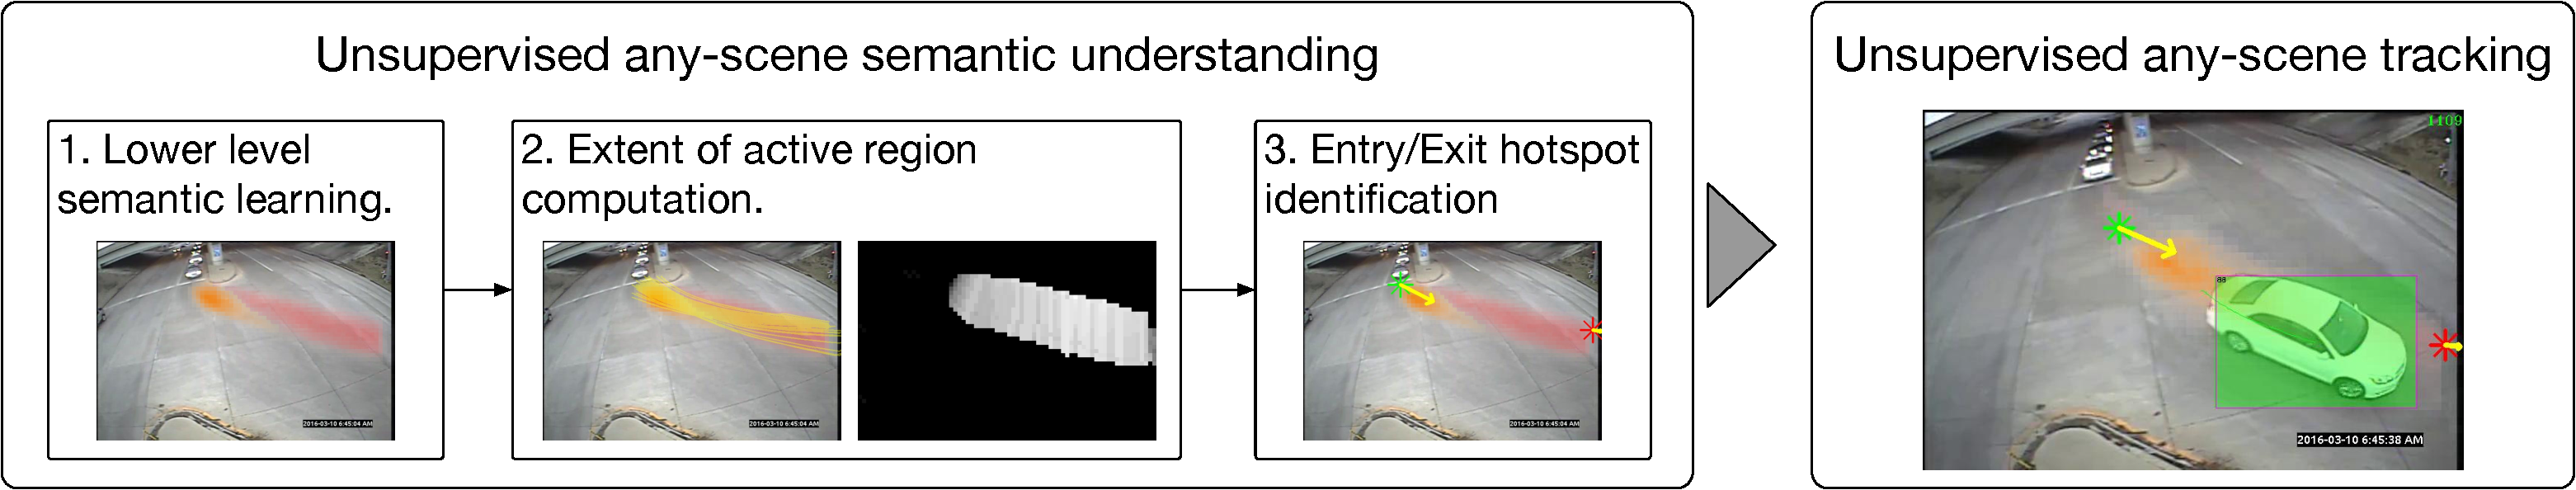
\includegraphics[width=\linewidth]{./img/scene_learning/workflow.pdf}
    \caption{System overview. The left corresponds to scene learning module: frequent motions are extracted in an unsupervised fashion, then the active regions where most objects move are learned on top of the motion result. Next, the entry/exit hotspot and their direction are extracted, describing how most objects enter and exit the scene. On the right, the semantic knowledge is applied to a tracker.}
    \label{fig:scene-workflow}
\end{figure}

\subsection{Non-parametric clustering via \gls{hdp}}
\label{subsec:hdp-bag-of-words}
For the general purpose of scene learning, lower-level representation could be a much more robust feature due to the difficulty of obtaining an accurate higher-level result, such as consistent object trajectories. A cluster of such low-level data as pixel movement could be an informative summary.
Inspired by the previous work \cite{wang2009unsupervised,kuettel2010s}, motion patterns can be learned by topic model, with an analogous bag-of-words representation to document classification.

Videos are processed as described in \ref{fig:scene-visual-doc}: first every frame is divided into small grids --- small enough to have consistent optical flow results. 
To distinguish different motions, optical flows of consecutive frames are quantized on $D$ directions after some simple filtering \cite{kalal2010forward}. 
Making an analogy with to document clustering, on a certain frame, each optical flow at a grid coordinate $(x, y)$ on a quantized direction is a \emph{visual word}.
If the frame is divided into $w\times h$ grids, the vocabulary is $V = w\times h\times D$.
% To understand what a visual topic is, it is crucial to know how the video is represented in the topic model.
% Even the grid could be smaller and $D$ be even larger, the corresponding vocabulary size could also slow down the sampling algorithm of topic models. 
As shown in the middle column of \ref{fig:scene-visual-doc}, the videos are then split temporarily into short video clips. 
Each video clip has enough frames to contain a complete motion, at the same time, is not too long to have mixed motions. 
By counting the number of visual words on each grid and each quantized direction in every video clip, we have a bag-of-words representation of \emph{visual documents}. 
Similarly, a cluster trained from the video could be called \emph{visual topic}.
%Note that the bag-of-words representation treats each word independently. 
\begin{figure}
\centering
    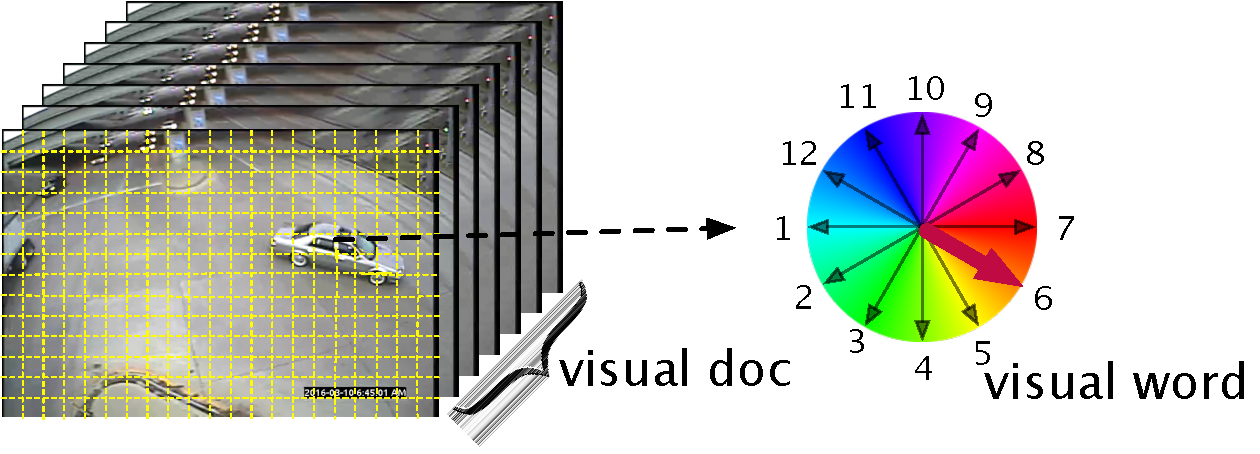
\includegraphics[width=0.8\linewidth]{./img/scene_learning/visual_doc.pdf}
    \caption{Left column illustrates the spatial and temporary quantization of video frames. The right shows a visual word obtained by discretizing the optical flow direction.}
    \label{fig:scene-visual-doc}
\end{figure}

% Using the bag-of-words representation, motions could be learned by any existing topic model method. 
% In most clustering methods, the number of clusters should be provided, and the results may vary according to the number of clusters. 
% Considering our goal to avoid unnecessary human input, we use the non-parametric model \gls{hdp} \cite{yee2006hierarchical} that required no specification of cluster numbers.
% It is a generalization of \gls{dp}. 
% In this model, the visual words are groups of observations, each exhibiting a mixed proportion of shared mixture components, also called "topics." 
% An HDP is a two-level \gls{dp} with shared parameters. Each group $j$ is associated with a draw from a shared \gls{dp} whose base distribution is also a draw from the top-level \gls{dp}.
% \begin{align}
% G_0 & \sim DP(\gamma, H) \\
% G_j|G_0 & \sim DP(\alpha_0, G_0), \qquad \text{for each }j.
% \end{align}

% Here $j$ is the group index. 
% At the top-level, the distribution $G_0$ is drawn from a \gls{dp} with concentration parameter $\gamma$ and base distribution $H$. 
% The base distribution $H$ is a symmetric Dirichlet over the vocabulary simplex. Since the numbers drawn from a Dirichlet distribution sum up to 1, they are usually used as the parameter of a multinomial distribution. 
% Each atom is a distribution over the vocabulary, the atoms $\mathbf{\phi} = (\phi_k)_{k=1}^{\infty}$ are drawn independently $\phi_{k}\sim \text{Dirichlet}(\eta)$. 
% Simply speaking, $G_0$ is a discrete distribution over the atoms $\mathbf{\phi}$. 
% At the bottom level, $G_0$ is used as the base distribution to draw each group distribution $G_j$. 
% By such hierarchical definition, the atoms are shared among $G_j$, which makes sense that different documents may belong to the same topic.
% In this setting, a group is a visual document and the $i$th word is drawn from $j$th document $x_{ji}$ as follows,
% $$\theta_{ji}\sim G_j, \qquad x_{ji}\sim\text{Multi}(\theta_{ji}).$$

% Here $\theta_{ji}$ is the topic assignment of $x_{ji}$, which is associated with a multinomial distribution $\phi_{\theta_{ji}}$. 
% One could potentially have an infinite number of atoms. However, only a finite number of atoms/topics are be learned. 
% After Gibbs sampling, there is a multinomial distribution for each topic over the vocabulary where each word in a document has a topic assignment. 
% \ref{fig:scene-topics} visualizes those topics learned by HDP. 
% The color indicates the direction shown in the color wheel on the right and the lightness indicates the value of the multinomial at the corresponding cell. 
% To make it clear, a topic distribution is a multinomial distribution over the entire vocabulary, that is to say, each grid has $D$ values in the multinomial distribution. 
% For simplicity, we only visualize the maximal value on each grid. 
% The Figures show that HDP does a good job in summarizing the motions in the video, even without knowing any moving objects in the scene. For more details on Gibbs sampling, please see \cite{yee2006hierarchical}.
% With some relaxation of term use, we also call it \emph{the density on the main direction}.
Using the bag-of-words representation, motions could be learned by any existing topic model method. 
In most clustering methods, the number of clusters is required as an input, and the results usually vary accordingly. For complex videos, it is presumably hard for people to identify the number of major motions. Therefore the non-parametric clustering method ---\gls{hdp} is used. 
It is a generalization of \gls{dp}, requiring no specification of the cluster number. 
In this model, visual words contain groups of observations, each exhibiting a mixed proportion of shared mixture components. 
The mixture components are learned in this model, also called "topics". 
More specifically, an \gls{hdp} is a two-level \gls{dp} with shared parameters. Each group $j$ is associated with a draw from a shared \gls{dp} whose base distribution is also a draw from the top-level \gls{dp}.
% In most clustering method, the results are sensitive to the number of clusters. Therefore, we naturally turn to Hierarchical Dirichlet Process (HDP), which is a non-parametric clustering method requiring no specification of cluster numbers. Figure \ref{fig:hdp} gives an graph illustration of HDP, Equation (\ref{eq:hdp}) gives mathematical formulation. We refer reader to \cite{yee2006hierarchical} for more details.
% \begin{figure} 
%     \center
%     \includegraphics[width=0.8\columnwidth]{./img/hdp.pdf}
%     \caption{Graph of HDP.}
%     \label{fig:hdp}
% \end{figure}
\begin{equation}    \label{eq:hdp}
\begin{aligned}    
    G_0 & \sim \text{DP}(\gamma, H) \\
    G_j|G_0 & \sim \text{DP}(\alpha_0, G_0), \text{for each } j,\\
\end{aligned}
\end{equation}
Here $j$ is the group index. At the top-level, the distribution $G_0$ is drawn from a \gls{dp} with concentration parameter $\gamma$ and base distribution $H$. 
The base distribution $H$ is a symmetric Dirichlet over the vocabulary simplex. 
Each atom is a distribution over the vocabulary, the atoms $\bm{\phi}=(\phi_k)^{\infty}_{k=1}$ are drawn independently $\phi_k \sim\text{Dirichlet}(\eta)$. Since the numbers drawn from a Dirichlet distribution sum up to 1, they are usually used as the parameters of a multinomial distribution. 
Simply speaking, $G_0$ is a discrete distribution over the atoms $\bm{\phi}$. 
At the bottom level, $G_0$ is used as the base distribution to draw each group distribution $G_j$, each is another multinomial distribution over the atoms $\bm{\phi}$. 
By such hierarchical definition, the atoms are shared among $G_j$, which makes sense that different documents may belong to the same topic.

In our setting, a group is a visual document and the $i$th word of the $j$th document $x_{ji}$ is drawn as follows:
\begin{equation}    \label{eq:multinomial}
\begin{aligned}
    \theta_{ji} = \phi_{z_{ji}}, \quad \theta_{ji}|G_j \sim G_j, \quad
    x_{ji}|\theta_{ji} \sim \text{Multi}(\theta_{ji})\\
\end{aligned}
\end{equation}
Here $z_{ji}$ is the topic assignment of $x_{ji}$, each word is associated with a multinomial distribution $\theta_{ji}$ according to its topic $z_{ji}$. 
We could potentially have an infinite number of atoms. However, only a finite number of atoms/topics are learned. 
After Gibbs sampling, there is a multinomial distribution for each topic over the vocabulary where each word in a document has a topic assignment. 
In other word, words in the same document may belong to  \emph{different} topics. \ref{fig:scene-topics} visualizes those topics learned by HDP. 
The color indicates the direction shown in the color wheel on the right and the lightness indicates the value of the multinomial at the corresponding grid. 
The Figures show that HDP does an excellent job of summarizing the motions in the video, even without knowing any moving objects in the scene. 
For more details on the model and Gibbs sampling, please see \cite{yee2006hierarchical}. 
\begin{figure}
    \begin{subfigure}{0.32\linewidth}
        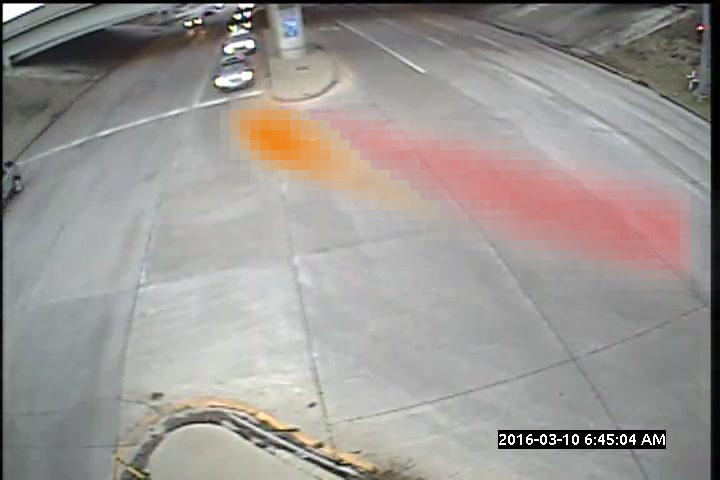
\includegraphics[width=\linewidth]{./img/scene_learning/topics/topic-1.jpg}
    \end{subfigure}%
    \begin{subfigure}{0.32\linewidth}
        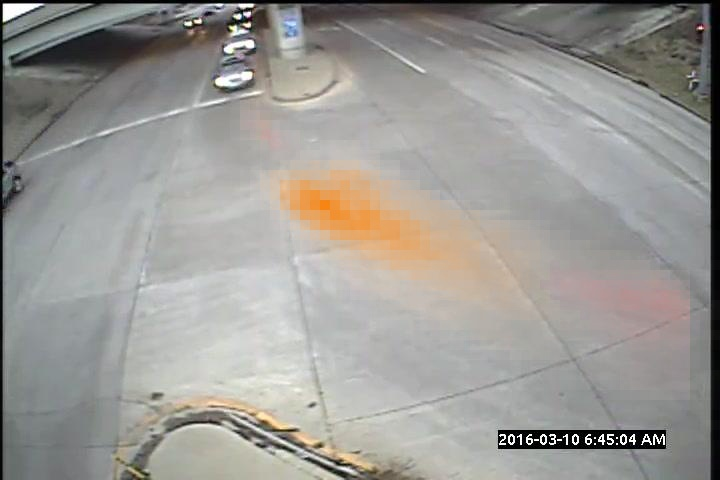
\includegraphics[width=\linewidth]{./img/scene_learning/topics/topic-3.jpg}
    \end{subfigure}%
    \begin{subfigure}{0.32\linewidth}
        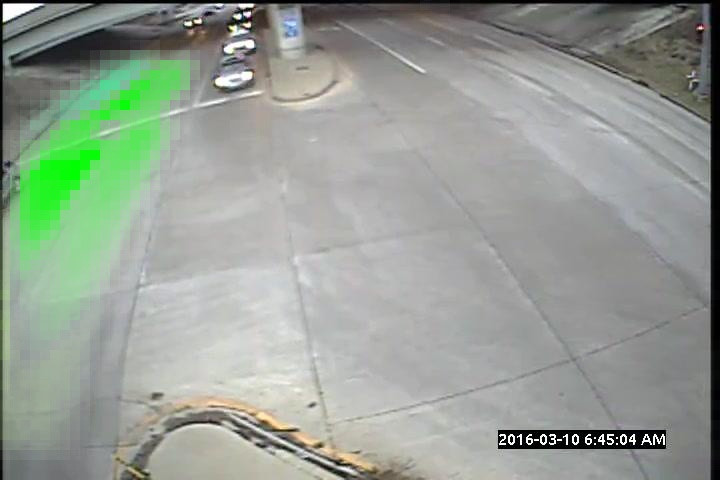
\includegraphics[width=\linewidth]{./img/scene_learning/topics/topic-0.jpg}
    \end{subfigure}%

    \begin{subfigure}{0.32\linewidth}
        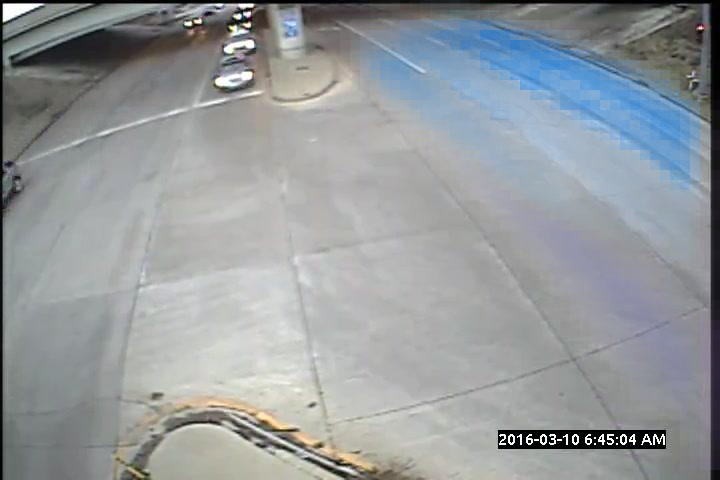
\includegraphics[width=\linewidth]{./img/scene_learning/topics/topic-2.jpg}
    \end{subfigure}%
    \begin{subfigure}{0.32\linewidth}
        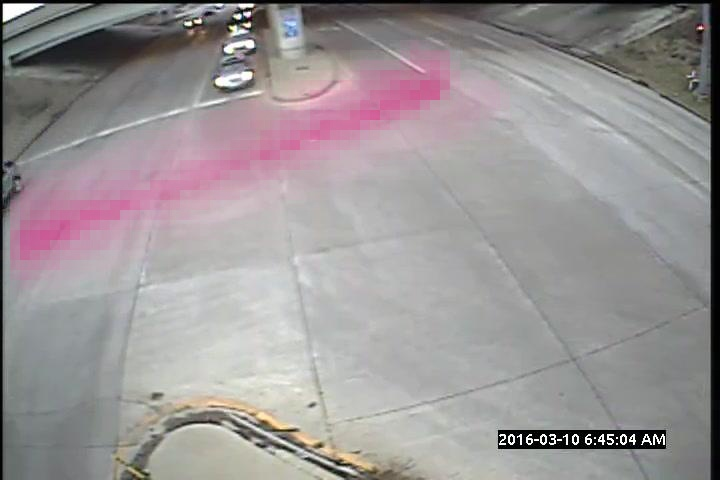
\includegraphics[width=\linewidth]{./img/scene_learning/topics/topic-4.jpg}
    \end{subfigure}%
    \hspace{0.08\linewidth}
    \begin{subfigure}{0.16\linewidth}
        
\includegraphics[width=\linewidth]{./img/scene_learning/color_wheel.png}
    \end{subfigure}
    \caption{Motions learned by HDP, colors indicate directions as the color wheel shows, the lightness indicate the magnitudes of the maximal probability values..}
    \label{fig:scene-topics}
\end{figure}

\section{Semantic knowledge learning}
\label{sec:scene-ridge-climbing}
The results generated by \gls{hdp} are several clusters of visual words, however, without any semantic meaning.
This section describes some post-processing steps for extracting higher-level semantic knowledge of the camera scene.

\subsection{Robust ridge climbing}
    Just by looking at the topics in \ref{fig:scene-topics}, we can roughly infer how the vehicles move in the video. 
    More importantly, the extent of the high-density grids gives useful insights into the size and moving region of the tracked objects. 
    Let $\phi$ be a multinomial distribution of a topic learned by \gls{hdp}. For any grid $i$, it has $D$ values, corresponding to $D$ evenly quantized directions, written as $\bm{\phi}_i= [\phi_i^{1}, \phi_i^{2}, \dots, \phi_i^{D}]$.
    We define two terms:
    $d^*_i = \argmax_{d}(\phi_i^{d})$ is the \emph{dominate direction} of grid $i$, which has the maximal value of distribution among all directions.
    We also define a terms summing over all the directions of each grid $\varphi_{i} = \sum_{d=1}^{D}{\phi_i^{d}}$.
    Figure \ref{subfig:scene-grid-dist} shows an example of the distribution of a particular topic on a grid, where the radius of each sector indicates the value of $\phi_i^{d}$. 
    In this topic, the grid has the highest $\phi_i^d$ with $d=1$, indicating that it is most likely to move along this direction. 
    \ref{fig:scene-ridge-clibming} gives a 3D visualization of the first topic in \ref{fig:scene-topics}, where the height at each grid is $\varphi_{i}$. 
    Overall they form a mountain-like surface. We aim to learn the shape and extent by extending the ridge climbing method in \cite{zhao2013counting}. 
    The idea of this method is to start from a high-density grid, make one step iteratively until reaching the image boundary or the low-density area. 
    The steps move along the desired direction and follow the shape of the topic distribution. 
    For consistency, all the following examples are on the first topic in \ref{fig:scene-topics}.
    % Due to the different views of the videos, some topics may expand a wide area, resulting ridge, not in the center of the high-density area. Accordingly, we improve this method by getting multiple ridges and then shrink them into a more confident center line.
    \begin{figure}
\centering
    \begin{subfigure}{0.48\linewidth}
        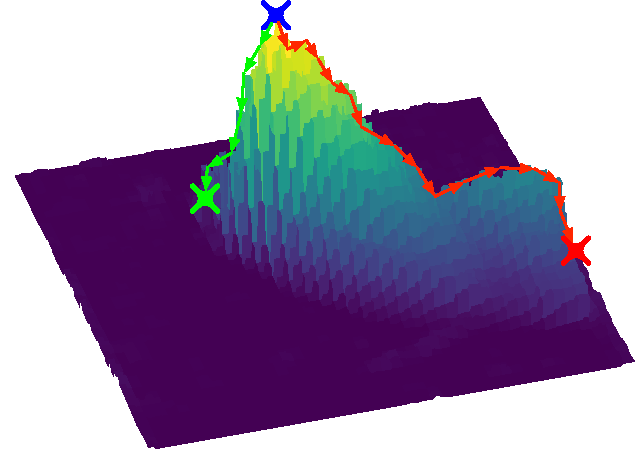
\includegraphics[width=\linewidth]{./img/scene_learning/ridge_climbing.pdf}
        \subcaption{}
        \label{subfig:scene-ridge-climbing}
    \end{subfigure}
    \begin{subfigure}{0.48\linewidth}
        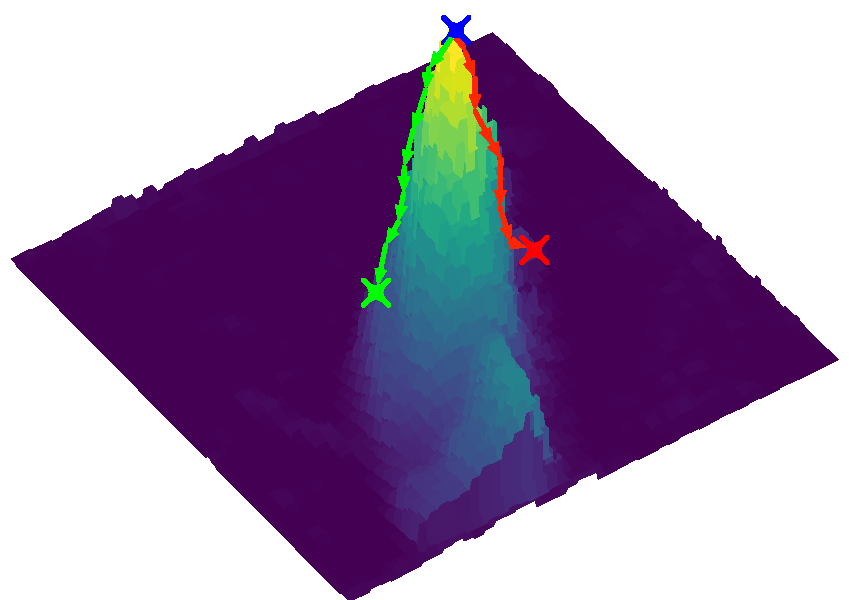
\includegraphics[width=\linewidth]{./img/scene_learning/ridge_climbing_perp.pdf}
        \subcaption{}
        \label{subfig:scene-ridge-climbing-perp}
    \end{subfigure}%
    \caption{3D visualization of the distribution of the first topic in \ref{fig:scene-topics} and ridge climbing illustration on it: along the dominant topic direction (\subref{subfig:scene-ridge-climbing}) and its perpendicular direction (\subref{subfig:scene-ridge-climbing-perp}). Blue cross indicates the starting point, red and green point indicates the end point.}
    \label{fig:scene-ridge-clibming}
\end{figure}
    % Automatic entry/exit point learning is rarely addressed in the current literature. \cite{makris2005learning} proposed a Mixture of Gaussian (MOG) methods to cluster start and end point of trajectories. However, this method is quite sensitive to noises. \cite{zhao2013counting} proposed a more robust ridge climbing method, given the HDP result above. Here we proposed an improvement of it based on sampling, adapting to more complicated videos.
    \begin{figure}
\centering
    \begin{subfigure}{0.26\linewidth}
        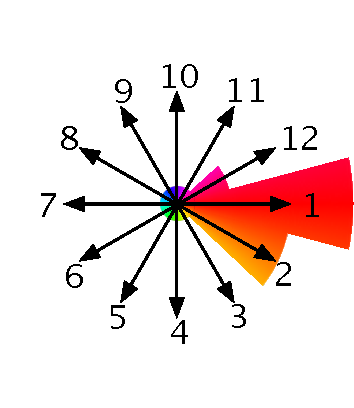
\includegraphics[width=\linewidth]{./img/scene_learning/grid_distribution.pdf}
        \subcaption{}
        \label{subfig:scene-grid-dist}
    \end{subfigure}
    \begin{subfigure}{0.35\linewidth}
        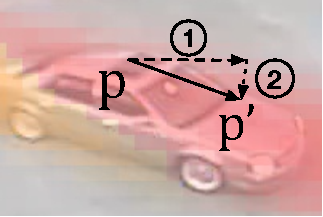
\includegraphics[width=\linewidth]{./img/scene_learning/step.pdf}
        \subcaption{}
        \label{subfig:scene-step}
    \end{subfigure}
    \begin{subfigure}{0.35\linewidth}
        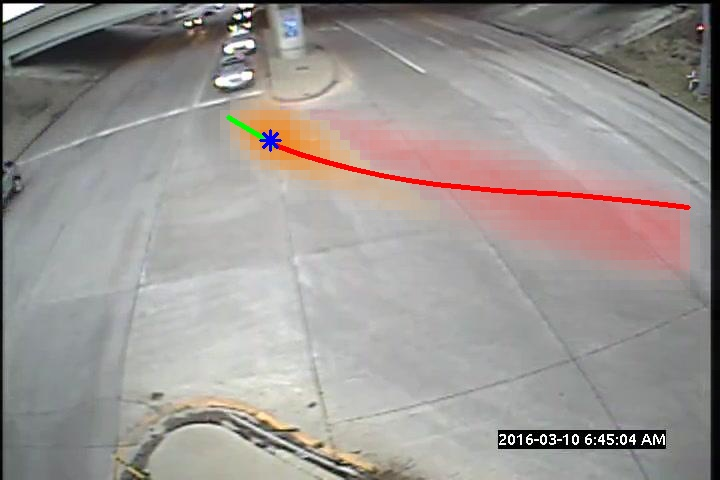
\includegraphics[width=\linewidth]{./img/scene_learning/single_ridge-1.jpg}
        \subcaption{}
        \label{subfig:scene-single-ridge}
    \end{subfigure}%
    \caption{(\subref{subfig:scene-grid-dist}) is an example of the topic distribution on one grid $i$, where the radius of each circle sector indicates $\bm{\phi}_i= [\phi_i^{1}, \phi_i^{2}, \dots, \phi_i^{D}]$. (\subref{subfig:scene-step}) shows the move-adjust step of each iteration. (\subref{subfig:scene-single-ridge}) is an extracted ridge starting from the highest density grid, where the blue star indicates the highest density grid, green and red line indicates ridges to the start/end point separately.}
    \label{fig:scene-step}
\end{figure}

    We propose a two-step movement in each iteration: first, we take a step, the step size is the normalized mean density on all the direction in its neighborhood; second, we adjust the step by moving toward higher density area. 
    The above steps are illustrated in Figure \ref{subfig:scene-step}, represented in dash lines, the final step is in solid line. 
    Mathematically, the two-step movement from $\bm{p}$ to $\bm{p^*}$ is represented as:
    \begin{align}
        \bm{p}' =&\bm{p} + \frac{\bm{v}}{||\bm{v}||_2}, \quad
        & \bm{v} = & \frac{\sum_{i=1}^n{ f(\bm{\omega})\cdot\bm{\phi}_i}}{{\sum_{i=1}^n{\varphi_i}}}, \label{eq:move}\\
        \bm{p}^* =& \bm{p}' + \alpha\cdot \bm{m}, \quad
        & \bm{m} = &\frac{\sum_{j=1}^n{\varphi_j\times(\bm{p}_i-\bm{p}')}}{\sum_{j=1}^n{\varphi_j}}.\label{eq:adjust}
    \end{align}
    We define a $2\times D$ matrix $\bm{\omega} = [\bm{\omega}_1, \bm{\omega}_2, \dots, \bm{\omega}_D]$, each column $\bm{\omega}_{d}$ is the unit vector along the quantized direction $d$.
    $\bm{v}$ and $\bm{m}$ correspond to the move and adjust step, separately. 
    For the move step \ref{eq:move}, $f(\bm{\omega})$ defines movement of each $\bm{\omega}_d$ wrt. a desired moving direction, which is the same size with $\bm{\omega}$. 
    Here we choose a neighborhood with $n$ grids around $\bm{p}$, and $\bm{p}_{i}$ is the coordinate of the $i$th grid in the neighborhood. 
    Therefore, $f(\bm{\omega})\cdot\bm{\phi}_i$ is the mean direction weighted by densities on each direction. 
    However, the moving step may not follow the elongated shape of the topic due to the uncertainty introduced by the quantized direction, where an example is given in Figure \ref{subfig:scene-step}. 
    To deal with it, we make an adjustment on the result of the move step \ref{eq:adjust}, once reaching a lower density area, $\bm{m}$ pulls the point back to the higher-density area and make the final step (solid arrow in Figure \ref{subfig:scene-step}) better follow the shape of the topic, as illustrated in step 2 in Figure \ref{subfig:scene-step}.
    Note that in the adjust step, we compute a new neighborhood around the result of the move step.
    Intuitively, if we reach a grid that has significantly different densities, we tend to take a smaller step in case the step size is too large to follow the density surface. 
    On the contrary, if the first step reaches a grid with a roughly uniform distribution around, $\bm{m}$ tends to be a zero vector and does not affect the final step.
    Due to the normalization term, $\bm{v}$ and $\bm{m}$ has magnitude at most $1$ in (\ref{eq:move}) and (\ref{eq:adjust}). 
    To make sure the adjust step does not cancel out the movement of step one, we normalize $\bm{v}$ into a unit vector. By setting $\alpha\in(0,1)$, it has a fixed impact on the final step. We observe that $\alpha\in[0.1,0.2]$ gives a reasonable result.

    Figure \ref{subfig:scene-ridge-climbing} gives an visual illustration of the ridge climbing process along the dominant direction, and Figure \ref{subfig:scene-single-ridge} shows the resulting ridge. The process starts from the grid with the highest $\varphi$, indicated by the blue cross, along the dominant direction, in this case, direction 1. 
    The red line is the path to the end point of the ridge, with $f(\bm{\omega}) = \bm{\omega}$; while the green line reaches the start point, obtained by setting $f(\bm{\omega}) = -\bm{\omega}$. So far the results are similar with those in \cite{zhao2013counting}.

    \begin{figure}
\centering
    % \begin{minipage}{0.48\linewidth}
    \begin{subfigure}{0.32\linewidth}
        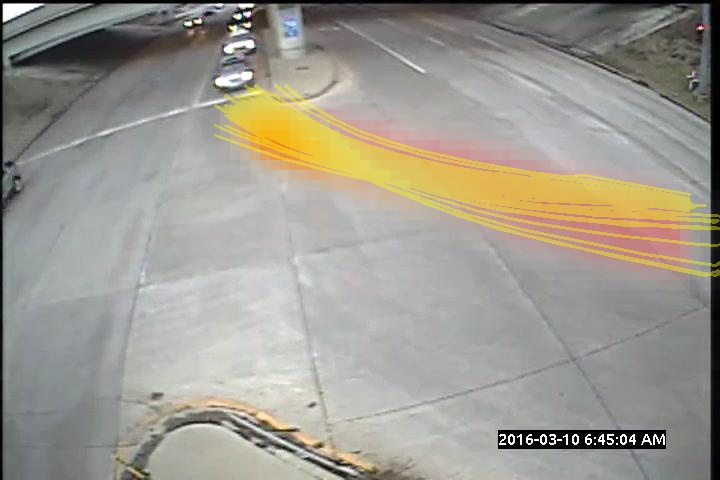
\includegraphics[width=\linewidth]{./img/scene_learning/ridges-1.jpg}
        \subcaption{}
        \label{subfig:scene-ridges}
    \end{subfigure}
    \begin{subfigure}{0.32\linewidth}
        
\includegraphics[width=\linewidth]{img/scene_learning/perp_width-1.png}
        \subcaption{}
        \label{subfig:scene-perp-width}
    \end{subfigure}
    \begin{subfigure}{0.32\linewidth}
        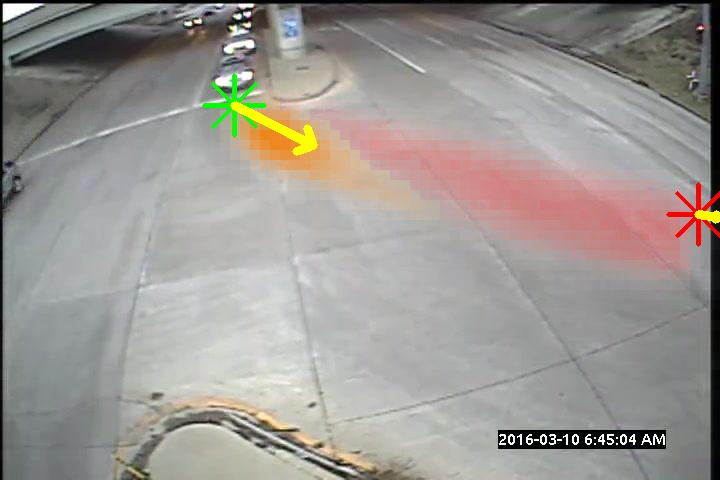
\includegraphics[width=\linewidth]{./img/scene_learning/res/middle/middle-1.jpg}
        \subcaption{}
        \label{subfig:scene-entry-exit}
    \end{subfigure}%
    \caption{(\subref{subfig:scene-ridges}): multiple ridges learned from local maximal grid. (\subref{subfig:scene-perp-width}): perpendicular width, where lighter intensity indicates a larger width. (\subref{subfig:scene-entry-exit}): extracted entry/exit hotspots indicates by the green and red star. And the yellow arrow shows their direction.}
    \label{fig:scene-ridge-res}
    % \end{minipage}
\end{figure}

% add a connection: the ridge is a single line, cannot capture the actual stripes traveled by vehicles and the dynamics of the changes in the stripe sizes. 
\subsection{Topic extent learning}
    Intuitively, the high-density grids indicate an active region when objects are more likely to move.
    A single ridge is not descriptive enough, especially for wide motion regions. 
    We propose two variations of the above procedure.
    First, instead of starting from the grid with global maximal $\varphi$, we start with multiple grids with local maximal $\varphi$ in its neighborhood. 
    The yellow lines in Figure \ref{subfig:scene-ridges} show the ridges extracted by the above procedure, where they roughly cover the high-density area. 
    Second, we define a \emph{perpendicular width} as the extent of the high density grids that perpendicular to the dominate direction. To obtain it, we climb the density surface along the direction perpendicular to the dominate direction $d^*_i$of the current grid $i$, demonstrated in Figure \ref{subfig:scene-ridge-climbing-perp}.
    $f(\bm{\omega})$ is obtained by rotating each unit vector $\bm{\omega}_{d}$ by 90 degrees clockwise ($f_1(\bm{\omega})$) and counterclockwise ($f_2(\bm{\omega})$). In other words, 
    \begin{align*}
        f_1(\bm{\omega}) = \left[\begin{array}{cc} 0 & -1\\ 1 & 0\end{array}\right]\cdot\bm{\omega},\quad
        f_2(\bm{\omega}) = \left[\begin{array}{cc} 0 & 1\\ -1 & 0\end{array}\right]\cdot\bm{\omega}.
    \end{align*}
    Figure \ref{subfig:scene-perp-width} shows the learned perpendicular width of the same topic, where the lighter color indicates a larger width. The ridges and the perpendicular width together define the active region of a topic, giving size, location and direction of the belonging objects.
    % Adjusting the neighborhood size may result in ridges with different densities and extensions. Using a finer quantization of visual words on 12 directions makes it possible to trace the ridges in arbitrary directions.


\subsection{Entry/exit hotspots extraction}
\label{subsec:hdp-entry-exit}
Compared with a single ridge, ridges start from multiple locations and better indicate the start and end of motions due to their larger coverage.  The density of extracted ridges gives a nice interpretation of the area and it is unlikely for vehicles to go beyond the topic area. 
For a set of ridges $\{\bm{l}_1, \bm{l}_2, \dots, \bm{l}_m\}$, 
each of $\bm{l}_i$ is a sequence of grid coordinates $\bm{l}_i=\{\bm{p}_i^1, \bm{p}_i^2, \dots, \bm{p}_i^{s_i}\}$, 
where $s_i$ is the length of ridge $\bm{l}_i$. 
We take the first and last point of each ridge, call them \emph{candidates} of the entry/exit hotspot. Formally defined as 
$$\mathbf{Z}_\text{entry} = \{\bm{p}_1^1, \bm{p}_2^1, \dots, \bm{p}_m^1\},\; \quad
\mathbf{Z}_\text{exit} = \{\bm{p}_1^{s_1}, \bm{p}_1^{s_2}, \dots, \bm{p}_1^{s_m}\}.$$
Similarly, each has its own direction: 
\begin{align*}
\mathbf{V}_\text{entry} =& \{\bm{p}_1^2 -\bm{p}_1^1, \dots, \bm{p}_m^2-\bm{p}_m^1\},\\
\mathbf{V}_\text{exit} = &\{\bm{p}_1^{s_1}-\bm{p}_1^{s_1-1}, \dots, \bm{p}_{m}^{s_m}-\bm{p}_{m}^{s_m-1}\}.
\end{align*}
Averaging over the coordinations and directions of candidates, we have a mean location and direction for each entry and exit hotspot: 
\begin{align}
\bm{p}_{entry} = \frac{\sum_{i=1}^m{\bm{p_i^1}}}{m},\;\quad&\bm{v}_{entry} = \frac{\sum_{i=1}^m{\bm{p_i^2}-\bm{p_i^1}}}{m},\\
\bm{p}_{exit} = \frac{\sum_{i=1}^m{\bm{p_i^{s_m}}}}{m},\;\quad&\bm{v}_{exit} = \frac{\sum_{i=1}^m{\bm{p_i^{s_m}}-\bm{p_i^{s_m-1}}}}{m}.
\end{align}
\ref{subfig:scene-entry-exit} gives an visual result of the above process, 
where the green and red star corresponds to $\bm{p}_{entry}$ and $\bm{p}_{exit}$, the yellow arrow shoes their directions $\bm{v}_{entry}$ and $\bm{v}_{exit}$.
% It is worth noting that the ellipses do not indicate the size of the entry/exit area, but the area most source/sink points fall in.
Although entry/exit hotspots are also able to be obtained by fitting the start/end points of trajectories, they are less reliable than statistics learned from lower-level representation, since we are working on a tracking framework.

% \subsection{Road Skeleton}
% Next, we apply the Adaptive Multi-Kernel-based Shrinkage (AMKS) method \cite{xu2015unsupervised} to the extracted ridges, which is originally proposed for trajectory clustering. Roughly speaking, it is a clustering method in a certain direction. In this case, it is specific to the moving direction of the motions. In every iteration, each ridge moves toward the center. Ideally, after convergence, all the ridges move to one centerline. Then the overlapped line is extracted as the final road skeleton. Before clustering, the overlapped ridges are filtered to reduce the computation overhead. The blue line in the right image in \ref{fig:scene} gives an example, where the dot at the right end indicates the sink. 
% \textcolor{red}{may discard it if not used by the tracker.}
\section{Semantic knowledge visualization}

For topic model training, we make each video clip 90 frames ($\sim$ 3 sec); each frame is divided into $10\times10$ pixel grids. Different from $D=4$ in \cite{wang2009unsupervised,kuettel2010s}, we make $D=12$. This number considers motions more than horizontal and vertical, making subsequent post-processing more accurate. 
We extend a C++ implementation of HDP \footnote{Chong Wang, David Blei: https://github.com/blei-lab/hdp.} and train the models on IDOT dataset \cite{yanziVehicleTracker}, each video is around 5 minutes. 
In the following, we first give some examples of the scene learning results, then see how the semantic knowledge helps improve object tracking.

Complementing the partial results in previous sections, \ref{fig:entry-exit-full-1}, \ref{fig:entry-exit-full-2} and \ref{fig:entry-exit-full-3} provide complete results on several scenes, 
with the same representation as previous sections.
\ref{fig:entry-exit-full-1} summarizes a low-resolution video, where the four main motions are captured, however, some turning motions may be missed. This is likely because optical flow with small magnitude is filtered as error before it is fed to the topic model, or because such motions are rare or do not appear in the training video.
For higher resolution videos, such as \ref{fig:entry-exit-full-2} and \ref{fig:entry-exit-full-3}, optical flow results are more accurate and movement magnitudes are greater, when measured in pixels. Consequently, HDP can catch most visible motions, and even distinguish individual lanes.
By visual inspection, the obtained movements, as well as the locations and directions of entry/exit points, are consistent with the subject scenes. 

\begin{figure}
    \centering
        \begin{subfigure}{0.32\linewidth}
            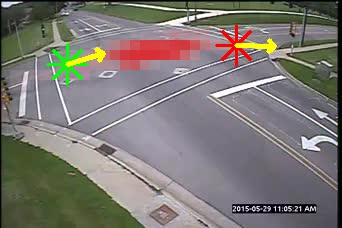
\includegraphics[width=\linewidth]{./img/scene_learning/res/244458/244458-0.jpg}
        \end{subfigure}
        \begin{subfigure}{0.32\linewidth}
            \includegraphics[width=\linewidth]{./img/scene_learning/res/244458/244458-1.jpg}
        \end{subfigure}

        \begin{subfigure}{0.32\linewidth}
            \includegraphics[width=\linewidth]{./img/scene_learning/res/244458/244458-2.jpg}
        \end{subfigure}
        \begin{subfigure}{0.32\linewidth}
            \includegraphics[width=\linewidth]{./img/scene_learning/res/244458/244458-3.jpg}
        \end{subfigure}
        \caption{Scene learning results at an intersection with one-way road. Entry (green) and exit (red) locations with direction (yellow arrows).}
        \label{fig:entry-exit-full-1}
\end{figure}

\begin{figure}
    \centering
        \begin{subfigure}{0.32\linewidth}
            \includegraphics[width=\linewidth]{./img/scene_learning/res/middle/middle-1.jpg}
        \end{subfigure}
        \begin{subfigure}{0.32\linewidth}
            \includegraphics[width=\linewidth]{./img/scene_learning/res/middle/middle-3.jpg}
        \end{subfigure}
        \begin{subfigure}{0.32\linewidth}
            \includegraphics[width=\linewidth]{./img/scene_learning/res/middle/middle-0.jpg}
        \end{subfigure}
        \begin{subfigure}{0.32\linewidth}
            \includegraphics[width=\linewidth]{./img/scene_learning/res/middle/middle-2.jpg}
        \end{subfigure}
        \begin{subfigure}{0.32\linewidth}
            \includegraphics[width=\linewidth]{./img/scene_learning/res/middle/middle-4.jpg}
        \end{subfigure}
        \caption{Scene learning results at a multi-way intersection. Entry (green) and exit (red) locations with direction (yellow arrows).}
        \label{fig:entry-exit-full-2}
\end{figure}

\begin{figure}
    \centering
        \begin{subfigure}{0.32\linewidth}
            \includegraphics[width=\linewidth]{./img/scene_learning/res/diverseyWestern/diverseyWestern-0.jpg}
        \end{subfigure}
        \begin{subfigure}{0.32\linewidth}
            \includegraphics[width=\linewidth]{./img/scene_learning/res/diverseyWestern/diverseyWestern-1.jpg}
        \end{subfigure}
        \begin{subfigure}{0.32\linewidth}
            \includegraphics[width=\linewidth]{./img/scene_learning/res/diverseyWestern/diverseyWestern-2.jpg}
        \end{subfigure}

        \begin{subfigure}{0.32\linewidth}
            \includegraphics[width=\linewidth]{./img/scene_learning/res/diverseyWestern/diverseyWestern-3.jpg}
        \end{subfigure}
        \begin{subfigure}{0.32\linewidth}
            \includegraphics[width=\linewidth]{./img/scene_learning/res/diverseyWestern/diverseyWestern-4.jpg}
        \end{subfigure}
        \begin{subfigure}{0.32\linewidth}
            \includegraphics[width=\linewidth]{./img/scene_learning/res/diverseyWestern/diverseyWestern-5.jpg}
        \end{subfigure}
        \caption{Scene learning results at a crowded multi-way intersection. Entry (green) and exit (red) with direction (yellow arrows).}
        \label{fig:entry-exit-full-3}
\end{figure}
\section{Discussion}

There remains some interesting aspects that can be potentially helpful for better scene understanding.
First, it maybe be worth some effort of a better choice of hyper-parameters, such as grid size, number of quantized directions, video clip length, length training video, maximal sampling iterations.
Grid size is related to the frame size. It is may not be necessary to have the same grid size for videos with different resolutions, since smaller grid size results in a larger vocabulary and a longer training time.
For videos with only horizontal and vertical motions, the optical flow quantization can be sparser. 
The video clip length may also need to adjust depending on different scenarios: ideally, we expect a video clip to cover a complete lifetime of single motion; shorter clip may break a topic into different parts while a longer video clip may generate a topic with mixed motions. 
Also, we have consider the traffic density of the scene to choose the size of the training data.
A scene with little traffic needs a longer training video than a crowded one.
However, even though the topic model is trained on a longer video, some rare motions may still be missing.


In addition, adding constraints among visual words might be necessary for some busy interactions. 
A ``topic'' is interpreted as a cluster containing ``words'' that always appear together, where the ``words'' are treated independently.
For an intersection with bi-directional movements all the time, the movement on both direction is naturally clustered as a single ``topic''. 
However, under the context of a video, the ``visual words'' are spatially and temporarily connected. 
If a ``visual topic'' is defined with only a single motion, the ``visual words'' one the opposite direction should be mutually exclusive.
\ref{fig:entry-exit-fail-1} and \ref{fig:entry-exit-fail-2} show two failure cases. 
One or more topics contain mixed motions, since those motion always happen simultaneously in the training data.
\begin{figure}
    \centering
        \begin{subfigure}{0.32\linewidth}
            \includegraphics[width=\linewidth]{./img/scene_learning/res/243653/243653_h264_0-0.jpg}
        \end{subfigure}
        \begin{subfigure}{0.32\linewidth}
            \includegraphics[width=\linewidth]{./img/scene_learning/res/243653/243653_h264_0-1.jpg}
        \end{subfigure}
        \begin{subfigure}{0.32\linewidth}
            \includegraphics[width=\linewidth]{./img/scene_learning/res/243653/243653_h264_0-2.jpg}
        \end{subfigure}
        \caption{Failure case with simultaneous opposite directions. Entry (green) and exit (red) locations with direction (yellow arrows).}
        \label{fig:entry-exit-fail-1}
\end{figure}
\begin{figure}
    \centering
        \begin{subfigure}{0.32\linewidth}
            \includegraphics[width=\linewidth]{./img/scene_learning/res/251950/251950-0.jpg}
        \end{subfigure}
        \begin{subfigure}{0.32\linewidth}
            \includegraphics[width=\linewidth]{./img/scene_learning/res/251950/251950-1.jpg}
        \end{subfigure}

        \begin{subfigure}{0.32\linewidth}
            \includegraphics[width=\linewidth]{./img/scene_learning/res/251950/251950-2.jpg}
        \end{subfigure}
        \begin{subfigure}{0.32\linewidth}
            \includegraphics[width=\linewidth]{./img/scene_learning/res/251950/251950-3.jpg}
        \end{subfigure}
        \caption{Failure case with simultaneous opposite directions. Entry (green) and exit (red) with direction (yellow arrows) at a crowded intersection.}
        \label{fig:entry-exit-fail-2}
\end{figure}


However, if the training video is carefully chosen, this problem may be avoided.
\ref{fig:entry-exit-night-1} and \ref{fig:entry-exit-night-2} are visualization of two models trained on a night video with sparse traffic. 
\ref{fig:entry-exit-night-1} is trained on a 5-minutes video, and \ref{fig:entry-exit-night-2} is trained on a 30-minutes video.
Topics in \ref{fig:entry-exit-night-2} have a better interpretation of the scene because the training video has sparse traffic at night. 
Since the video contain little traffic, there is less likely to have simultaneous movement in the opposite direction.
A longer video has much more sufficient data for training.
\begin{figure}
    \centering
        \begin{subfigure}{0.32\linewidth}
            \includegraphics[width=\linewidth]{./img/scene_learning/res/elstonIrvingPark-short/20150829_020000DST_elstonIrvingPark-0.jpg}
        \end{subfigure}
        \begin{subfigure}{0.32\linewidth}
            \includegraphics[width=\linewidth]{./img/scene_learning/res/elstonIrvingPark-short/20150829_020000DST_elstonIrvingPark-1.jpg}
        \end{subfigure}
        \begin{subfigure}{0.32\linewidth}
            \includegraphics[width=\linewidth]{./img/scene_learning/res/elstonIrvingPark-short/20150829_020000DST_elstonIrvingPark-1.jpg}
        \end{subfigure}

        \begin{subfigure}{0.32\linewidth}
            \includegraphics[width=\linewidth]{./img/scene_learning/res/elstonIrvingPark-short/20150829_020000DST_elstonIrvingPark-3.jpg}
        \end{subfigure}
        \begin{subfigure}{0.32\linewidth}
            \includegraphics[width=\linewidth]{./img/scene_learning/res/elstonIrvingPark-short/20150829_020000DST_elstonIrvingPark-4.jpg}
        \end{subfigure}
        \caption{Model training on sparse night video about 5 minutes. Entry (green) and exit (red) locations with direction (yellow arrows).}
        \label{fig:entry-exit-night-1}
\end{figure}
\begin{figure}
    \centering
        \begin{subfigure}{0.32\linewidth}
            \includegraphics[width=\linewidth]{./img/scene_learning/res/elstonIrvingPark/20150829_020000DST_elstonIrvingPark-0.jpg}
        \end{subfigure}
        \begin{subfigure}{0.32\linewidth}
            \includegraphics[width=\linewidth]{./img/scene_learning/res/elstonIrvingPark/20150829_020000DST_elstonIrvingPark-1.jpg}
        \end{subfigure}

        \begin{subfigure}{0.32\linewidth}
            \includegraphics[width=\linewidth]{./img/scene_learning/res/elstonIrvingPark/20150829_020000DST_elstonIrvingPark-2.jpg}
        \end{subfigure}
        \begin{subfigure}{0.32\linewidth}
            \includegraphics[width=\linewidth]{./img/scene_learning/res/elstonIrvingPark/20150829_020000DST_elstonIrvingPark-3.jpg}
        \end{subfigure}
        \caption{Model training on sparse night video about 30 minutes. Entry (green) and exit (red) locations with direction (yellow arrows).}
        \label{fig:entry-exit-night-2}
\end{figure}


However, it does not always work for tuning training videos. 
If a busy intersection always have the opposite movement at the same time, the learned topics tend to contain mixed movement.
We considered introducing such exclusion into \gls{hdp} via Hierarchical \gls{ddcrp} \cite{blei2011distance}.
Due to the limited time, we do not completely finish this part.
\chapter{Semantic Tracker}
\label{chp:semantic-tracker}

\section{Introduction}
\label{sec:semantic-intro}
\section{Object motion assignment}
\label{sec:semantic-inf}

The offline training phase generates models for the \emph{visual topic}, where the inference on the videos from the same camera helps identify the topic assignment of a tracked object before any topic-specific constraints are applied.
To do inference, first, we need to make the frame the same format as the \emph{visual document}.
We maintain a small sliding window of consecutive frames close to the current one, as well as its bag-of-words representation, same as in \S\ref{subsec:hdp-bag-of-words}.  
The sliding window is across multiple frames; therefore, it takes the temporal consistency into account and is more robust than a single frame.

After inference, each visual word $x$ is assigned to the topic with the maximal probability. 
Then we reduce the results temporarily and spatially to the granularity of the grids on the frame.
Assume $v_{x}$ is the index of $x$ in the vocabulary. 
Each word index may have multiple counts considering the bag-of-words representation being a histogram.
We take the result of majority voting as the topic assignment $k_v$ of the word index $v$ as following:
\begin{align}
k_{v} = \argmax_k{\sum_{x\in\{x:v_{x} = v\}}{\mathbf{1}(k_{x} = k)}},
\end{align}
where $\mathbf{1}(\cdot)$ is the indicator function.
On the other hand, each grid maps to $D$ word index in the vocabulary, indicating $D$ directions in \ref{fig:scene-visual-doc}.
Similarly, we could reduce the topic statistics to grids by majority voting.
\begin{align}
k_{g} = \argmax_k{\sum_{v\in\{v:g_{v} = g\}}{\mathbf{1}(k_v = k)}},
\end{align}
where $g_{v}$ is the grid that word index $v$ locates, and $k_g$ is the topic assignment of grid $g$ in that frame.
When there comes a bounding box of interest, its topic assignment can be determined by the majority voting of topics of the covered grids.
We omit the inference detail here; for details, we refer the reader to \cite{yee2006hierarchical}.

Here the underlying assumption of the reduction is that each grid belongs to only one movement, which is a reasonable case on a single frame.
If the sliding window is small, all of the words on the same grid are likely to have the same topic assignment.
Therefore, the majority voting rules out some unusual cases where some $v$ has little counts.
Another benefit of these methods is that since the inference is done on words level, it captures the correct topic assignment even with mixed topics in the scene.
\section{Tracking score}
Based on the life span of a tracked object, there are three stages: initialization, tracking, and termination. 
Most literature focuses on tracking, assuming initialization and termination are properly handled.
However, for practical use, each stage should be carefully dealt with to ensure performance. 
For the first time, we introduce applying the scene-specific semantic knowledge to object tracking throughout the objects' lifetime. 
\subsection{Initialization}     
    An object being ``out of scene'' actually refers to two scenarios: out of image boundary or too small to be recognized. Without loss of generation, this corresponds to both two cases when objects enter and exit the scene, as an example given in \ref{fig:semantic-entry-exit}. 
    These two cases may be problematic for tracker initialization and termination if not handled correctly. An object may either be initialized when being partially visible or too small to be recognized. 
    Different from the standard object tracking framework, tracking task in real-world use usually relies on external algorithms to find object candidates. Consequently, it is a critical step to the overall performance of any related surveillance task.
    In the following, we show how we apply the scene semantic knowledge into the tracking process and deal with the two scenarios above with a uniform affinity measurement. 

    \begin{figure}
\centering
    \begin{subfigure}{0.4\linewidth}
        \includegraphics[width=\linewidth]{./img/semantic_tracker/193402-entry-exit-0.jpg}
        \subcaption{}
        \label{subfig:semantic-extry-exit-eg1}
    \end{subfigure}
    \begin{subfigure}{0.4\linewidth}
        \includegraphics[width=\linewidth]{./img/semantic_tracker/193402-entry-exit-3.jpg}
        \subcaption{}
        \label{subfig:semantic-extry-exit-eg2}
    \end{subfigure}%
    \caption{Two scenarios of object enters and exits: (\subref{subfig:semantic-extry-exit-eg1}): objects enter with a tiny size and move out of image boundary; (\subref{subfig:semantic-extry-exit-eg2}): objects enter from the image boundary and exit with a tiny size in within the frame. Green and red star are the obtained entry/exit hotspots; yellow arrows shows their direction.}
    \label{fig:semantic-entry-exit}
\end{figure}
    
    In the computer vision field, for a rigid object, it is widely accepted to use a rectangle as the representation of an object: $\bm{r} = [x, y, w, h]$, where $\bm{p_r}=(x, y)$ is the coordinates of the center point and $(w, h)$ is the width and height.
    A straight line through point $\bm{p}$, parallel to vector $\bm{v}$ is define as $L(\bm{p}, \bm{v})$. Similarly, a ray from point $\bm{p}$ in the direction of vector $\bm{v}$ is define as $R(\bm{p}, \bm{v})$.
    For a rectangle $\bm{r}$ with a center point $\bm{p_r}$, given its moving direction $\bm{v_r}$, we have the following terms for the rectangle, also visually illustrated in Figure \ref{subfig:semantic-box-perp-width} and Figure \ref{subfig:semantic-last-pt}:  
    \begin{itemize}
        \item \emph{Perpendicular width:} the distance between two intersection points of line $L(\bm{p_r}, \bm{v}_{\bm{r}\cdot\text{perp}})$ and the rectangle $\bm{r}$, written as $W(\bm{r}, \bm{v_r})$. 
        \item \emph{Last point:} the intersection point of ray $R(\bm{p_r}, \bm{-v_r})$ with the rectangle $\bm{r}$, written as $P(\bm{r}, \bm{v_r})$.
    \end{itemize}
    Here $\bm{v}_{\bm{r}\text{perp}}$ is the vector perpendicular to $\bm{v_r}$, such that $\bm{v_r}\cdot\bm{v}_{\bm{r}\text{perp}}=0$. Since the object's aspect ratio may vary with the object type and view point of the camera, by defining the \emph{perpendicular width}, both width and height are taken into account. As we will show in the following, the definition of \emph{last point} has a better interpretation of object's moving process, specifically for entering and exiting the scene.

    \begin{figure}
\centering
\begin{subfigure}{0.27\linewidth}
    \includegraphics[width=\linewidth]{./img/semantic_tracker/box_perp_width.pdf}
    \subcaption{}
    \label{subfig:semantic-box-perp-width}
\end{subfigure}
\begin{subfigure}{0.27\linewidth}
    \includegraphics[width=\linewidth]{./img/semantic_tracker/last_pt.pdf}
    \subcaption{}
    \label{subfig:semantic-last-pt}
\end{subfigure}
\begin{subfigure}{0.42\linewidth}
    \includegraphics[width=\linewidth]{./img/semantic_tracker/last_pt_dist.pdf}
    \subcaption{}
    \label{subfig:semantic-last-pt-dist}
\end{subfigure}%
\caption{All the solid pink arrows above indicate the moving direction $\bm{v_r}$, the pink dot is the center of the rectangle, blue dots are the intersection points with the rectangle. (\subref{subfig:semantic-box-perp-width}): perpendicular width $W(\bm{r}, \bm{v_r})$ of the object's bounding box wrt. to  direction $\bm{v}_{r}$, shown as the blue dash line. \subref{subfig:semantic-last-pt}: last point $P(\bm{r}, \bm{v_r})$ of the object's bounding box $\bm{r}$, where the dash arrow is $R(\bm{r}, \bm{-v_r})$. (\subref{subfig:semantic-last-pt-dist}): distance between a hotspot with a rectangle's center point and last point $P(\bm{r}, \bm{v_r})$, shown in pink and blue dash lines.}
\label{fig:semantic-perp-width}
\end{figure}

    In real-world applications, with no pre-determined object initialization available, applications usually rely on methods such as background subtraction and object detector, which usually tend to be error-prone.
    With the learned semantic knowledge, we only initialize objects that are around the entry area of the current available topics, with consistent direction and reasonable size. Consequently, noisy candidates with inconsistent motions or far away from the entry area will be effectively eliminated. 
    % \begin{align}
    %     S_\text{dist}(\bm{p}, \bm{p}_1, \bm{p}_2) & = \frac{D\left(\bm{p}, \bm{p}_1\right)}{D\left(\bm{p}_1, \bm{p}_2\right)} \label{eq:entry_dist}\\
    %     S_\text{size}(x_1, x_2) & = 1 - \frac{|x_1 - x_2|}{x_1 + x_2} \label{eq:entry_size}\\
    %     S_\text{direction}(\bm{v}_1, \bm{v}_2) & = \cos(\bm{v}_1, \bm{v}_1) \label{eq:direction}
    % \end{align}

    To quantitatively represent the affinity of an object to a topic $k$'s entry area, we define the following metric:
    \begin{align}
        \begin{split}
        S_\text{entry}(\bm{r}, k) = \frac{1}{3}\times & \Bigl[\Bigl(1-\frac{D(P(\bm{r}, \bm{v_r}), \bm{p}_k(\text{entry}))}{D(\bm{p}_k(\text{entry}), \bm{p}_k(\text{exit}))}\Bigl) \\
        + & \left(1 - \frac{|W(\bm{r}, \bm{v_r}) - W_k(\bm{p_r})|}{W(\bm{r}, \bm{v_r}) + W_k(\bm{p_r})}\right) \\
        + & \cos\big(\bm{v_r}, \bm{v}_k(\text{entry})\big)\Bigl]\label{eq:entry_score}
        \end{split}
    \end{align}
    Here $D(\cdot)$ is the distance measurement of two arbitrary points, we simply use Euclidean distance here. 
    $\bm{p}_k(\text{entry})$ and $\bm{p}_k(\text{exit})$ are the entry and exit point of topic $k$, where the entry/exit points are the Gaussian mean obtained in \S\ref{subsec:hdp-entry-exit}. 
    $W_k(\bm{p_r})$ and $\bm{v}_k(\bm{p_r})$ are the perpendicular width and main direction of topic $k$ at location $\bm{p}_{r}$.
    
    The first term in the square parenthesis is the distance of $P(\bm{r}, \bm{v_r})$ to the exit point, relative to the entry point. It produces a high value for bounding boxes around the entry area, taking the extent of the topic into account without placing any hard threshold. 
    Note that instead of using the center of the rectangle $\bm{p}_{r}$, we use the last point of it. 
    As illustrated in Figure \ref{subfig:semantic-last-pt-dist}, when computing the distance of the object's bounding box and the hotspot, with the moving direction available, considering the last point along the direction measures the movement of the entire object. In other words, despite various object size, by ensuring the last point close to the entry/exit area, the entering/exiting process completes for the entire object.
    The second term will be close to 1 if and only if $W(\bm{r}, \bm{v_r})$ and $W_k(\bm{p_r})$ are similar.
    This penalizes bounding boxes of size either too large or too small, making sure the qualified candidate has a reasonable size relative to the topic's perpendicular width. 


    % Second, as stated in \cite{yanziVehicleTracker}, tracking should start after the object becomes large enough, with more stable and trackable movement. Optical flows are filtered before clustering; therefore, error-prone optical flows do not fall in the entry area extracted on such motion topics.   

    To deal with objects close to the image boundary, we do not initialize a tracker until the last point of the bounding box $\bm{r}$ is apart from the image boundary at least a margin distance; for an object enters with a tiny size, initialization is not considered when the object movement $||\bm{v_r}||_2$ equals $0$, since tiny size usually indicates tiny movement.
    Satisfying the above two cases, we initialize an object with a bounding box $\bm{r}$ once $S_{\text{entry}}(\bm{r}, k) > \sigma_{1}$ for a certain $k$. 

\subsection{Termination}
    When the tracked object manages to reach the exit area, it is quite likely to be well tracked, due to our checking scheme described later in \S\ref{sec:track_eval}. Therefore, we consider terminating a tracker once it is close to its topic's exit area. 
    Similarly, we define a distance measurement of a rectangle $\bm{r}$ with its exit area:
    \begin{align}
        S_\text{exit}(\bm{r}, k) = 1-\frac{D\left(P(\bm{r}, \bm{v_r}), \bm{p}_k(\text{exit})\right)}{D\left(\bm{p}_k(\text{entry}), \bm{p}_k(\text{exit})\right)}
    \end{align}
    where we think the object passes through its exit area when $S_\text{exit}(\bm{r}, k) > \sigma_2$.
    However, in case the object is still able to be correctly tracked, we mark it and keep tracking until it gets lost, we call this phase \emph{extended tracking}. 
    The final trajectory is until the object gets lost. This is especially useful when the object exists with a tiny size. Due to the filtering of the topic model training process, tiny movements are filtered as noises. However, when the object can be tracked beyond the exit zone, it is better to keep a longer trajectory. 

\subsection{Tracking quality evaluation}
\label{sec:track_eval}
An object's size, location, and motion are well constrained once we have a topic assignment of it. 
Once we initialize a tracker, we check the tracking quality on every frame. In general, we want objects to move smoothly and follow its visual topic. To quantitatively evaluate this, we define a smoothness term for an object's scale change:
\begin{align}
    S(\bm{r}_1, \bm{r}_2) = \frac{1}{2}\left[\left(1-\frac{|w_1- w_2|}{w_1 + w_2}\right) + \left(1-\frac{|h_1 - h_2|}{h_1 + h_2}\right)\right], 
\end{align}
here $w_i$ and $h_i$ are the width and height of rectangle $\bm{r}_{i}$, separately. $S(\bm{r}_1, \bm{r}_2)$ makes sure there is no abrupt scale change between two consecutive frames.
Besides that, to evaluate how well the object is tracked, we have to consider regular tracking and extended tracking differently. 
Before the object reaches its exit area, it is supposed to follow the corresponding visual topic tightly, possibly with occasional stops. So the tracking score is defined as:
\begin{align}
\begin{split}
    S_{\text{track}}(\bm{r}, k, t) = \frac{1}{3}\Bigl[\left(1 - \frac{|W(\bm{r}_t, \bm{v}_{\bm{r}_t}) - W_k(\bm{p}_{\bm{r}_t})|}{W(\bm{r}_t, \bm{v}_{\bm{r}_t}) + W_k(\bm{p}_{\bm{r}_t})}\right) \\
    + S(\bm{r}_t, \bm{r}_{t-1}) + \cos(\bm{v}_{\bm{r}_t}, \bm{v}_k(\bm{p}_{\bm{r}_t}))\Bigl]
\end{split}
\label{eq:track_score}
\end{align}

However, once the object passes through its exit area, it is expected to be terminated once it is not well tracked. 
Additionally, zero movements are not allowed. Since the object is not likely to pass through high-density grids in extended tracking phase, we compare the object's moving direction with the exit direction. A similar measurement is defined as:
\begin{align}
    S_{\text{extend}}(\bm{r}, k, t) = \frac{1}{2}\left[S(\bm{r}_t, \bm{r}_{t-1}) + \cos(\bm{v_r}, \bm{v}_k(\text{exit}))\right]\label{eq:track_ext_score}
\end{align}
In both measurement above, the notations are all similar with before, except that a subscript $t$ is added, indicating the corresponding variable at frame $t$. 
$\bm{v}_k(\bm{p}_{\bm{r}_t})$ and $\bm{v}_k(\text{exit})$ are the main direction of topic $k$ at $\bm{r}_{t}$'s center point $\bm{p}_{\bm{r}_t}$, and exit area.
A valid tracking is defined as $S_{\text{track}}(\bm{r}, k, t)>\sigma_{3}$ or $S_{\text{extend}}(\bm{r}, k, t)>\sigma_{4}$, depending on whether it has passed through its exit area. Unqualified tracking will be discarded as failures along the way.
By checking the tracking quality in this way, it is guaranteed that objects manage to pass the exit area follows its topic well and has a smooth movement and scale change. 
Empirically, $\sigma_1\sim\sigma_{4}$ between $0.7\sim0.8$ are a reasonable threshold.

\section{Semantic tracker}

\subsection{Semantic knowledge update}
With some successfully tracked objects, we may adaptively update the semantic scene. 
More specifically, we update the corresponding topics with well-tracked objects, which are those enter through the entry area, tightly follow its belonging topic, and successfully exit through exit areas. 
The scene is updated as follows: 
The first and last location, along with the direction of a high-quality trajectory is used to update the entry/exit candidates; the rectangle perpendicular width wrt. its topic is used to update the topic perpendicular within its extent, where the updated value remains the mean of all the updates.
By such iterative updating, we have more representative scene knowledge regarded to object tracking. The entry/exit area may gradually shift to where most objects enter and exit, where the perpendicular width of each topic also better fits the object statistics. The entire process is described in Algorithm \ref{alg:semantic-tracker} to \ref{alg:semantic-tracker-entry}.

\begin{algorithm}
 \caption{Tracking with semantic knowledge.}
 \label{alg:semantic-tracker}
 % \KwData{$K$ visual topics, corresponding entry/exit area and direction.}
 \begin{algorithmic}[1]
 \For{each frame $t$} 
     \State Topic model inference on the frame.
     \State Obtain foreground boxes $\mathbf{R}_{bg} = \{\bm{r}_{bg}\}$.
     \State Obtain detection boxes $\mathbf{R}_{det} = \{\bm{r}_{det}\}$.
     \For{each $i$ th object $O_i$ at $\bm{r}_{t-1}(i), \quad(i = 1, \dots, N_t)}$
        \State Get topic assignment $k_t(i)$.
        \State Find the most matched boxes $\bm{r}_{bg}(i)$ and $\bm{r}_{det}(i)$ with $\bm{r}_{t-1}(i)$.
        \State $\mathbf{R}_{bg} = \mathbf{R}_{bg}\setminus\bm{r}_{bg}(i), \mathbf{R}_{det} = \mathbf{R}_{det}\setminus\bm{r}_{det}(i).$
        \State Compute mean velocity $\bm{v}(i)$ within $\bm{r}_{t-1}(i)$ from the optical flow.
        \State Make measurement for tracking update $\bm{z}_t(i) = [\bm{r}_{bg}(i), \bm{r}_{det}(i), \bm{v}(i)]$.
        \State Set measurement covariance error $R$.
        \State Update object tracker with $\bm{z}_t(i)$ and $R$, get result $\bm{r}_{t}(i)$.
        \State CheckExitSemantic$(O_i, \bm{r}_t(i), k_t(i), t)$
     \EndFor
     \For{Each remaining box candidate $r\in\{\mathbf{R}_{bg}\bigcup\mathbf{R}_{det}\}$}
      \State CheckEntrySemantic$(\bm{r})$.
     \EndFor
\EndFor
\end{algorithmic}
\end{algorithm}

\begin{algorithm}
 \caption{CheckExitSemantic$(O, \bm{r}, k, t)$}
 \label{alg:semantic-tracker-exit}
 \begin{algorithmic}[1]
\If{$O$ is in extended tracking phase} 
  \If{$S_{\text{extend}}(\bm{r}, k, t) <=\sigma_{4}$}
    \State Exit object.
%             update semantic scene\;
  \EndIf
\ElsIf{$S_{\text{track}}(\bm{r}, k, t)<\sigma_{3}$} 
  \State Discard object.
\EndIf
\If{$S_\text{exit}(\bm{r}, k) > \sigma_2$} 
  \State Enter extended tracking phase.
\EndIf
\end{algorithmic}
\end{algorithm}

\begin{algorithm}
 \caption{CheckEntrySemantic$(\bm{r})$}
 \label{alg:semantic-tracker-entry}
 \begin{algorithmic}[1]
\State Get the topic $k$ for $\bm{r}$ at this frame.
\If{$S_\text{entry}(\bm{r}, k) > \sigma_{1}$}
  \State Initialize object.
\EndIf
\end{algorithmic}
\end{algorithm}

\section{Evaluation}
\label{sec:semantic-eval}

% \subsection{Entry/Exit Comparison with Ground Truth}

\subsection{Tracking accuracy}

The extracted movements and entry/exit locations are hard to evaluate quantitatively, due to a lack of both ground-truth and accepted difference metrics.
Instead, we extend a vehicle tracker with initialization- and update filters based on movements and entry/exit locations extracted from the scene, as described in the previous section.

\begin{figure}
    \centering
     \begin{subfigure}{0.48\linewidth}
    \includegraphics[width=\linewidth]{./img/semantic_tracker/exp/count_lowRes.pdf}
    \subcaption{Low resolution videos.}
    \end{subfigure}
    \begin{subfigure}{0.48\linewidth}
    \includegraphics[width=\linewidth]{./img/semantic_tracker/exp/count_highRes.pdf}
            \subcaption{High resolution videos.}
    \end{subfigure}
    \caption{The number of true positive and false positve trackers. The black lines mark the ground truth, the striped and black bar are the true positive and false positive, separately.}
    \label{fig:semantic-eval-count}
\end{figure}

\ref{fig:semantic-eval-count} shows our main result. Here, we compare the tracker from \cite{yanziVehicleTracker}, labeled {\it heuristic}, against our version extended with a scene learning filter, labeled {\it scene}. 
Although the {\it heuristic} tracker relies on several manually tuned parameters, this is one of the few benchmarks that quantitatively evaluate tracking including initialization and termination, which is critical for any realistic vehicle tracking application.

Here, true and false positives are based on matching tracked vehicles with ground truth trajectories.
We use the {\it overlap} of two rectangles, defined by the intersection over union for a rectangle box $\bm{r}$ and a ground truth $\bm{r}_0$,

$$\text{Overlap}(\bm{r}, \bm{r}_0) = \frac{A(\bm{r} \cap \bm{r}_0)}{A(\bm{r} \cup \bm{r}_0)},$$

averaged over the frames in which the ground truth trajectory or the tracking result occurs. 

As in \cite{yanziVehicleTracker}, we match each ground truth trajectory to the tracking result with the greatest overlap and use overlap $> 0.3$ to indicate a true positive. Any ground truth trajectories without a true positive match are considered false negatives, and any tracking result without a matched ground-truth trajectory with overlap > 0.3 is considered a false positive.
We find that our scene learning filter dramatically reduces false positives while keeping true positives essentially constant. 

A large number of false positives remain for the high-resolution videos. Due to the complex vehicle interactions in high the resolution video (see \ref{fig:entry-exit-full-3}), even with the semantic knowledge, the na\"ive Kalman Filter may easily lose track, resulting in an increased false positive count.

%We compare our scene-learning based tracker with the heuristic one, both with the setting that updated with background only and background along with detection, which we call BG and BG+DET. 
%According to the author, the dataset contains low-resolution videos with few occlusions and crowded high-resolution videos. We display their results separately for a better understanding of our method.

% \begin{itemize}
%         \item \textbf{Initialize}: A candidate rectangle $\bm{r}$ is not able to be initilialized with great overlap with any of the currently tracked objects $O_{\bm{r}}$, that is when $\text{IoU}(\bm{r}, O_{\bm{r}}) > 0.3$.
%         \item \textbf{Update}:An object $O_{\bm{r}}$ is updated with the rectangle $\bm{r}$ with the maximal $\text{IoU}(\bm{r}, O_{\bm{r}})$.
%         \item \textbf{Terminate}:Objects without update for 50 frames or out of image boundary are terminated.
%         \item \textbf{Validate}:Objects with lifetime longer than 50 frames and moves at last $\frac{1}{3}$ of the frame width is a good trajectory.
% \end{itemize}
% Here $\text{IoU}(\bm{r}_1, \bm{r}_2) = \frac{A(\bm{r}_1 \cap \bm{r}_2)}{A(\bm{r}_1 \cup \bm{r}_2)}$ is the widely used intersection over union metric. $\bm{r}_1 \cap \bm{r}_2$ and $\bm{r}_1 \cup \bm{r}_2$ representats the intersection and union separately, and $A(\cdot)$ simiply computes the area.

%With Eq. (\ref{eq:entry_score}), large number of candidate rectangles are filtered for initialization. In \ref{fig:filter-low} and \ref{fig:filter-high} shows the number of initialized and sucessfully tracked objects. For all the videos, semantic knowledge filters out up to $60\%$ more candidates than the heuristic tracker. 
%The successfully tracked object number proves the contribution of Eq. (\ref{eq:track_score}) and (\ref{eq:track_ext_score}) in filtering failed trackers. 
%% \begin{figure}
%%         \centering
%%          \begin{subfigure}{0.48\linewidth}
%%         \includegraphics[width=\linewidth]{./img/exp/filter_BG_GPU_lowRes.pdf}
%%         \subcaption{Low resolution videos.}
%%         \end{subfigure}
%%         \begin{subfigure}{0.48\linewidth}
%%         \includegraphics[width=\linewidth]{./img/exp/filter_BG_GPU_highRes.pdf}
%%         \subcaption{High resolution videos.}
%%         \end{subfigure}
%%         \caption{Initialization filtering for BG setting. The left group is heuristic tracker and the right is our tracker. The black bars are the number of objects initialized by background subtraction; the left striped bar is the sucessfully tracked objects number.}
%%         \label{fig:filter-low}
%% \end{figure}

%% \begin{figure}
%%         \centering
%%          \begin{subfigure}{0.48\linewidth}
%%         \includegraphics[width=\linewidth]{./img/exp/filter_BG+DET_lowRes.pdf}
%%         \subcaption{Low resolution videos.}
%%         \end{subfigure}
%%         \begin{subfigure}{0.48\linewidth}
%%         \includegraphics[width=\linewidth]{./img/exp/filter_BG+DET_highRes.pdf}
%%         \subcaption{High resolution videos.}
%%         \end{subfigure}
%%         \caption{Initialization filtering with BG+DET setting. The black and the right most bars in each group are the number of objects initialized by background subtraction and detector; the left striped bar is the sucessfully tracked objects number.}
%%         \label{fig:filter-high}
%% \end{figure}
%% The above figures show the semantic knowledge helps with eliminating noisy initializations and identifying tracking failure. 
%% Here we directly proves its improvement in tracking.
%% Ideally, a good tracker has true positives close to the ground truth, and false positives as few as possible.
%% \ref{fig:match} visualize the true positves and false positives of each tracker. 
%% Since there is no modification on the tracker self, it is reasonable that we don't have a significant change in true positives.
%% The scene knowledge integrated tracker maintains a roughly the same number of true positive, while dramatically reduces the false positive. 


%\subsection{Tracking accuracy}

\begin{figure}
    \centering
     \centering
     \begin{subfigure}{0.48\linewidth}
    \includegraphics[width=\linewidth]{./img/semantic_tracker/exp/success_lowRes.pdf}
    \subcaption{Low resolution videos.}
    \end{subfigure}
    \begin{subfigure}{0.48\linewidth}
    \includegraphics[width=\linewidth]{./img/semantic_tracker/exp/success_highRes.pdf}
            \subcaption{High resolution videos.}
    \end{subfigure}
    \caption{Success rate plot.}
    \label{fig:semantic-eval-success}
\end{figure}

\ref{fig:semantic-eval-success} shows the success plot of the two trackers for both simple and complex videos.
Here, the {\it success rate} is defined as the fraction ground-truth trajectories that have a minimum overlap with its matched tracking output.
Thus, the success rate measures how closely the matched trajectories actually match the ground truth.
The larger area under the curves is, the better the tracking is.
We see significant improvement in tracking accuracy with the help of scene learning, especially on the more complex videos.

%Without modification on the tracker, the improvement should come from a better initialization, which is consistent with the conclusion in \cite{yanziVehicleTracker}: for objects enters from the image boundary or coming from a tiny size, delaying the initialization could help improve the tracking performance.

In conclusion, we find that filtering tracker initialization and update using scene learning can significantly improve tracker performance, both in terms of precision and accuracy.  

%Our filtering criteria follow this conclusion in two ways: first, with the definition of the last point, objects are initialized only when it completely enters the image. That is to say, the corresponding tracker has richer information than the those initialized partially seen.
%Second, the topic model filters some noisy optical flows with tiny magnitude. 
%Therefore, the extracted entry location does not expand to a noisy area with small movements. Under our entry criteria, tiny objects are not initialized until passing through a more confident region.
%Further with the experiments on the state-of-the-art trackers in \cite{yanziVehicleTracker}, the author concludes that general purpose trackers could benefit from proper initialization. 
%We could further infer that our semantic learning integrated initialization and tracking framework could be potentially useful any trackers in real-world use. 


% \subsection{Analysis of Semantic Tracking}
% Compare the ratio of initialization with maximal ground truth area with our last paper result.

% \section{Related work}
% prior work that is competing, or even may be perceived to be similar by reviewers (similar names, let’s say). Mention most references only by group, like “group A [X, Y, Z, W] addresses problem 1”, then at the end of describing each group or an individual piece of work, try to contrast your work against it in one sentence. “By contrast, our method does not assume independence."

\label{sec:semantic-related}
% Human input fr surveillance tracker
To ensure the accuracy for practical use, most surveillance system heuristically relies on prior knowledge, such as a specific deployment of the cameras or human input. For example, by calibration with know camera specifications, \cite{cheng2011intelligent,corral2017slot} restores the real-world coordinates and infers the actual measurement of the tracked objects. Another type of work requires the area of interest for the tracked objects in advance, such as entry/exit area in \cite{tamersoy2009robust,rodriguez2010adaptive,mishra2013video}, and a skeleton of the road surface in \cite{bas2007automatic}. None of the above methods is easy to apply to new camera settings.

% scene learning: motion pattern and semantic areas.
To understand the scene in the videos, current work either learns the semantic areas or movement patterns. The former such as \cite{tung2011goal,nedrich2013detecting,yang2012multi} learn the entry/exit areas from the trajectories already available or on-the-fly. Such methods require robust trajectories, which may not always be available in practical use.
On the contrary, the latter \cite{wang2009unsupervised,kuettel2010s,hospedales2009markov,liao2015video} statistically learn the motions from the quantized optical flow, without knowledge of the actual objects in the scene, therefore, are more robust and flexible. 

% semantic tracking.
On the other hand, some researchers are working on the semantic aided tracking. \cite{zhao2012tracking,kratz2010tracking} use motion information to constrain the movement of the tracked objects; however, they are only for crowded scenes, since single object-trackers prefer appearance-based features.
There are also work exploring scene evidence from trajectories: either from existing trajectories \cite{song2010online} or hand-drawn artificial trajectories \cite{manen2014appearances}. However, reliable trajectories still remain an issue for real-world application.

Despite the robust results in Bayesian motion learning, little work has extended them to vehicle tracking.
Zhao \etc \cite{zhao2013counting} applies \cite{wang2009unsupervised} to vehicle counting. However, we still lack a general component for automatic initialization/termination to fit in the current tracking framework.

\chapter{Scene-specific Motion Model}
\label{chp:gp-ukf}

\section{Introduction}
\label{sec:gp-ukf-intro}

The underlying assumption in \S\ref{sec:tracker-kf} is that vehicles follow the constant acceleration model in a short period, like in the physical world.
However, everything in the scene experiences distortion due to projection in most traffic videos. Therefore, vehicles' movement does not follow the linear model in \ref{eq:kf-transition}, and a linear state model is insufficient for the Kalman Filter to capture the movement pattern of the vehicles in the scene.

When good observations are available consistently, Kalman filter can follow the tracked vehicle, even though the linear model cannot accurately reflect the size and velocity change. 
With missing observation or occlusion, the tracker is expected to predict with its internal model in the \emph{extrapolation} mode. 
However, with the linear model broken, the tracker can only generate reasonable results for a short period.

To tackle this problem, we proposed a \gls{ukf} tracker, which learns a non-linear model from the history trajectories by \gls{gp}. 
The semantic knowledge is the prerequisite of the non-linear model, which ensures the trajectories of high quality.
Under the constraints of semantic learning, every vehicle that survives to the exit hotspot is consistent with its motion topic in terms of entry/exit location, size, and velocity.

\section{Gaussian Process}
\label{sec:gp}
Gaussian Process is a non-parametric model that learns a distribution over functions $f\sim \mathcal{GP}$.
Given a dataset 
$\mathcal{D} = \left\{(\mathbf{x}_i, y_i), \mathbf{x}_i \in \mathbb{R}^d, y \in \mathbb{R}, i=1,\dots, N \right\}$, 
where $y_{i} = f(\mathbf{x}_i)$.
A \gls{gp} assumes a prior distribution that 
$f(\mathbf{x}_{1}), f(\mathbf{x}_{2}), \dots, f(\mathbf{x}_{N})$ 
jointly follows a Gaussian distribution $p(\mathbf{f}|\mathbf{X}) = \mathcal{N}(\mathbf{f}|\mathbf{\mu}, \mathbf{K})$,
where $\mathbf{K}_{ij}$ is defined by a kernel function $\mathbf{K}_{ij} = \kappa(\mathbf{x}_i, \mathbf{x}_j)$.
When $N_{*}$ new data points come, by the definition of GP, the joint distribution forms another Gaussian distribution
\begin{align}
\begin{pmatrix} \mathbf{y}\\ \mathbf{f_*}\end{pmatrix} \sim \mathcal{N}\left(
\begin{pmatrix} \mathbf{\mu} \\ \mathbf{\mu}_{*}\end{pmatrix}, 
\begin{pmatrix} \mathbf{K} && \mathbf{K}_*\\ \mathbf{K^T}_* && \mathbf{K}_{**}\end{pmatrix}
\right),
\end{align}
where $\mathbf{K}=\kappa(\mathbf{X}, \mathbf{X})$ is $N\times N$, $\mathbf{K}_*=\kappa(\mathbf{X}, \mathbf{X}_*)$ is $N\times N{*}$, and $\mathbf{K}_{**}=\kappa(\mathbf{X}_*, \mathbf{X}_*)$ is $N_*\times N_*$.

By the conditioning Gaussian \cite{rasmussen2003gaussian}, the posterior is $p(\mathbf{f}_*|\mathbf{X}, \mathbf{X}_*, \mathbf{y}) = \mathcal{N}(\mathbf{f}_*|\mathbf{\mu}_*, \mathbf{\Sigma}_*)$, where
\begin{align}
\mathbf{\mu}_* & = \mathbf{\mu(X_*)} + \mathbf{K}^T_*\mathbf{K}^{-1}(\mathbf{y-\mu(X)})\label{eq:gp-mu}\\
\mathbf{\Sigma}_* & = \mathbf{K_{**}-K_*^TK^{-1}K_*}
\label{eq:gp-cov}
\end{align}

For the regression task, we can use $\mathbf{\mu}_*$ as the prediction.
Usually we assume $\mathbf{\mu(X)} = 0, \mathbf{\mu(X)}_* = 0$. The \gls{rbf} kernel is used here
\begin{align}
\kappa(\mathbf{x}_i, \mathbf{x}_j) = \sigma_f^2 \exp\left(-\frac{1}{2}\sum_{d=1}^{D}\left(\frac{\mathbf{x}_{id}-\mathbf{x}_{jd}}{l_d}\right)^2\right).
\end{align}
We use a different length scale for each dimension of $\mathbf{x}$.
$\sigma_{f}$ and $l_{d}$ are hyper parameters of the GP learned through a optimization solver.

\subsection{Multiple output Gaussian Process}

\S\ref{sec:gp} introduces the basic definition of \gls{gp}, where $y$ is a real value.
However, in our case, we learn a scene-specific motion model, which is a mapping of vehicle states between two consecutive frames. 
The history trajectories provide such mapping for training and capture the non-linear movement.
Different from \S\ref{sec:tracker-kf}, we use a six-dimension input $\mathbf{x} = [x, y, w, h, x', y']$, which represents the location, size and velocity of vehicle. 
The output $\mathbf{y}$ has to have the same format with input $x$, as it becomes the input for the next frame.
Therefore, the single-output \gls{gp} extends to multiple output, where $\mathbf{y} \in \mathbb{R}^{6}$. 
The covariance matrix is shared among all dimensions, equivalent to several single-output \gls{gp} with the same 
covariance matrix.

\subsection{Online processing for streaming data}

One of the major challenges for \gls{gp} is the covariance matrix $\mathbf{K}$. 
$\mathbf{K}$ grows with the size of training data, while the cost of computing the inverse $\mathbf{K}^{-1}$ is $O(N^3)$.
On the other hand, we have streaming training data as the tracking continues. 
$\mathbf{K}$ need to be updated every time new data comes and every iteration of the optimization for the hyper-parameter.
$\mathbf{K}$ can become enormously large if we store all the data. 
\ref{fig:gp-ds} shows the relationship between the trajectory count and the training data count. 
The training data count grows linearly with the training trajectory.
With about 32 trajectories, the matrix $\mathbf{K}$ size reaches 2000. 
\begin{figure}
\centering
    \includegraphics[width=\linewidth]{./img/gp/gp-ds.pdf}
    \caption{The training data count grows linearly with the training trajectory count.}
    \label{fig:gp-ds}
\end{figure}

Therefore, we have to maintain the $\mathbf{K}$ to a reasonable size and avoid computing $\mathbf{K}^{-1}$ too frequently to balance the computation overhead.
Some filtering and forgetting policies are applied here.
First, we only add the data that has enough change over the previously added data point.
Here $L1$ distance is used to measure the difference. 
Similar trajectory record between adjacent frames is often seen when the tracked object remains static in the scene or is too small to have a large change of size or velocity.
Second, we run hyper-parameter optimization upon the first batch of training data arrive; later we run the optimization with a longer interval.
Finally, after the training data has reached the maximal number, every time a new data point becomes available, it is added with a possibility of $p = 0.7$ and a random old data point is removed.
Moreover, once the $\mathbf{K}^{-1}$ is computed, the prediction only involves simple matrix multiplication.
We implement the algorithm on GPU to have fast matrix operation.

As the tracking continues, the covariance matrix $\mathbf{K}$ is maintained to a fixed size. 
We also keep a separate thread for computing $\mathbf{K}^{-1}$ and hyper-parameter optimization. 
The thread runs in the background without interrupting the tracker.
The above methods ensure the tracker still run in real time.

\section{Unscented Kalman Filter}
In Kalman Filter, there are two important models, 
\begin{itemize}
\item Internal state model: $\mathbf{x}_t = f(\mathbf{x}_{t-1}, \mathbf{w}_{t-1})$
\item Observation model: $\mathbf{z}_t = h(\mathbf{x}_t, \mathbf{v}_t)$
\end{itemize}
where $\mathbf{x}_t$ and $\mathbf{z}_t$ are the internal state and the observation,
$\mathbf{w}_t$ and $\mathbf{v}_t$ are the process and measurement noise at time $t$, 
and both $f(\cdot)$ and $h(\cdot)$ are assumed linear. 
However, in many cases, at least one of the linear models does not hold. Therefore, methods for Kalman Filter with nonlinear model are proposed, including \gls{ekf} \cite{julier1997new} and \gls{ukf} \cite{wan2000unscented}. 
\gls{ekf} uses Taylor series expansion to approximate the nonlinearity, may introduce errors for the true mean and covariance of the state variables after the non-linear transformation.
Additionally, in our case, there is no close-formed nonlinear motion model under camera projection. 
Consequently, we use \gls{ukf}, where its nonlinear state model $f(\cdot)$ is learned by the non-parametric model \gls{gp}.

% \begin{figure}
\centering
\includegraphics[width=\linewidth]{./img/gp/ut.png}
\caption{Example of the UT for mean and covariance propagation. a) actual, b) first-order linearization (EKF), c) UT.}
\label{fig:ufk-ut}
\end{figure}

The key of \gls{ukf} is \gls{ut}, which calculates the statistics of random variables under a nonlinear transformation, accurately capturing the mean and the covariance to the 3rd order Taylor series expansion for Gaussian inputs. 
For a random variable $\mathbf{x} \in \mathbb{R}^{d}$ with mean $\bar{\mathbf{x}}$ and covariance $\mathbf{P_x}$, to calculate the statistics of $\mathbf{z}$ under a nonlinear mapping $\mathbf{z} = g(\mathbf{x})$, first a set of sigma points are built around the $\bar{\mathbf{x}}$ \cite{wan2000unscented},
\begin{align}
\begin{split}
\mathcal{X}_0 & = \bar{\mathbf{x}} \\
\mathcal{X}_i & = \bar{\mathbf{x}} + (\sqrt{(d+\lambda)\mathbf{P_x}})_i, \qquad i = 1, \dots, d\\
\mathcal{X}_i & = \bar{\mathbf{x}} - (\sqrt{(d+\lambda)\mathbf{P_x}})_i, \qquad i = d+1, \dots, 2d\\
W_0^{(m)} & = \lambda/(d+\lambda) \\
W_0^{(c)} & = \lambda/(d+\lambda) + (1-\alpha^2+\beta) \\
W_i^{(m)} & = W_i^{(c)} = 1/\{2(d+\lambda)\} \qquad i = 1, \dots, 2d
\end{split}
\end{align}

where $\alpha$ controls the spread of the sigma points around $\bar{\mathbf{x}}$, 
$\lambda = \alpha^{2}(d+\kappa)-d$ and $\kappa$ are the scaling parameters,
$\beta$ describe the prior knowledge for the distribution of $\mathbf{x}$.
$\alpha$ is usually set to a small value (\eg $1e-3$),
$\kappa$ is usually set to 0 and $\beta$ is optimally set to $2$ for Gaussian distribution.
$(\sqrt{(d+\lambda)\mathbf{P_x}})_i$ is the $i$th row of the matrix square root. 
Each sigma point is propagated through the nonlinear function $g(\cdot)$, 
$$\mathcal{Z}_{i} = g(\mathcal{X}_i) \qquad i = 0, 1, \dots, 2d,$$
The mean and covariance for $\mathbf{z}$ are approximated by the weighted sample mean and covariance of the posterior sigma points,
\begin{align}
\bar{\mathbf{z}} & \approx \sum_{i=0}^{2d}{W_i^{(m)}\mathcal{Z}_i}\\
\mathbf{P_z} & \approx \sum_{i=0}^{2d}{W_i^{(c)}(\mathcal{Z}_i-\bar{\mathbf{z}})(\mathcal{Z}_i-\bar{\mathbf{z}})^T}
\end{align}

Therefore, with the non-linear state and measurement model, \gls{ukf} naturally extends the unscented transformation by applying it alternately between the predict and correct step.
\section{GP-UKF tracker}
\label{sec:gp-ukf}

\subsection{Tracking}

In the tracking setting, the state model is a nonlinear \gls{gp} model while the measurement model is still linear.
\begin{align}
\mathbf{x}_t = & f(\mathbf{x}_{t-1}) = \text{GP}(\mathbf{x_{t-1}}, \mathbf{X}) \\
\mathbf{z}_t = & h(\mathbf{x}_t) = H\mathbf{x}_t,
\end{align}

Similar with \S\ref{sec:tracker-kf}, the observation is still the bounding boxes generated by background subtraction model and vehicle detector, and filtered pixel movement from optical flow: 
$$\mathbf{z}=[x^{bg}, y^{bg}, w^{bg}, h^{bg}, x^{det}, y^{det}, w^{det}, h^{det}, v_x, v_y].$$ 
Similarly, the measurement model $H$ is a $6\times10$ matrix with $1$ at $(0, 0),$ $(1, 1),$ $(2, 2),$ $(3, 3),$ $(0, 4),$ $(1, 5),$ $(2, 6),$ $(3, 7),$ $(4, 8),$ $(5,9)$.

A complete step of the GP-UKF tracker is described in Algorithm \ref{alg:gp-ukf}, which can be adapted to the semantic tracker by substitution of the tracking step in Algorithm \ref{alg:semantic-tracker}.
\begin{algorithm}
\caption{GP-UKF.}\label{alg:gp-ukf}
\begin{algorithmic}[1]
\Require {State transition mapping $\{\mathbf{x}_{t-1}, \mathbf{x}_{t}\}$ from history data.}
\State Start with $\hat{\mathbf{x}}_{0} = \mathbf{x}_{0}$.
\State Calculate the sigma points: $\mathcal{X}_{t-1} = \left[\hat{\mathbf{x}}_{t-1}, \hat{\mathbf{x}}_{t-1}\rpm\sqrt{(d+\lambda)P_{t-1}}\right]$.
\State Predict:
\State{$\begin{aligned} 
\hat{\mathcal{X}}_{i, t} = & \text{GP}_{\mu}(\mathcal{X}_{i, t-1}, \mathbf{X}), \quad i = 0, \dots, 2d\\
\hat{\mathbf{x}}_{t}^{\mhyphen} = & \sum_{i=0}^{2d}{W_i^{(m)}\hat{\mathcal{X}}_{i,t}} \\
P_{t}^{\mhyphen} = & \sum_{i=0}^{2d}{W_i^{(c)}[\hat{\mathcal{X}}_{i,t}-\hat{\mathbf{x}}_t^{\mhyphen}][\hat{\mathcal{X}}_{i,t}-\hat{\mathbf{x}}_t^{\mhyphen}]^T} \\
\hat{\mathcal{Z}}_t = & \left[H\hat{\mathcal{X}}_{i, t}\right], \quad i = 0, \dots, 2d\\
\hat{\mathbf{z}}_t^{\mhyphen} = & \sum_{i=0}^{2d}{W_i^{(m)}\hat{\mathcal{Z}}_{i,t}}
\end{aligned}$}
\State Get measurement covariance of $\mathbf{z}_{t}$: $ R_t = \text{GP}_{\sigma}(\mathbf{z}_t, \mathbf{X})$.
\State Correct with measurement:
\State {$\begin{aligned} 
P_{\hat{\mathbf{z}}_t, \hat{\mathbf{z}}_t} = & \sum_{i=0}^{2d}{W_i^{(c)}[\hat{\mathcal{Z}}_{i,t}-\hat{\mathbf{z}}_t^{\mhyphen}][\hat{\mathcal{Z}}_{i,t}-\hat{\mathbf{z}}_t^{\mhyphen}]^T} + R_t\\
P_{\hat{\mathbf{x}}_t, \hat{\mathbf{z}}_t} = & \sum_{i=0}^{2d}{W_i^{(c)}[\hat{\mathcal{X}}_{i,t}-\hat{\mathbf{x}}_t^{\mhyphen}][\hat{\mathcal{Z}}_{i,t}-\hat{\mathbf{z}}_t^{\mhyphen}]^T} \\
K = & P_{\hat{\mathbf{x}}_t, \hat{\mathbf{z}}_t}P_{\hat{\mathbf{z}}_t, \hat{\mathbf{z}}_t}^{-1}\\
\hat{\mathbf{x}}_t = & \hat{\mathbf{x}}_t^{\mhyphen} + K(\mathbf{z}_t-\hat{\mathbf{z}}_t^{\mhyphen})\\
P_t = & P_t^{\mhyphen} - KP_{\hat{\mathbf{z}}_t, \hat{\mathbf{z}}_t}K^T
\end{aligned}$}
\end{algorithmic}
\end{algorithm}

\subsection{Cold start}
Before any trajectory is available, we track vehicles automatically with the Kalman Filter with the linear model in \ref{sec:tracker-kf}. 
With some accumulated trajectories, the \gls{gp} can predict for objects with similar size and location.
However, the prediction may fail at some unseen data; therefore, it is necessary to assess the quality of the prediction.
We use the covariance of the data point in \ref{eq:gp-cov}, since it measures the certainty of the prediction. 
Upon initialization of an object, \gls{gp}-\gls{ukf} is used only when the obtained covariance is small ($< 0.1$); otherwise, the linear Kalman Filter is used.

% \subsection{Measurement covariance}
% Instead of manual hard-coded measurement covariance in \ref{sec:tracker-kf}, \gls{gp} also helps determine the measurement covariance.
% Similarly, we use \ref{eq:gp-cov} to determine the quality of a measurement covariance .


\section{Evaluation}

\ref{fig:kf-gp-1}, \ref{fig:kf-gp-2}, \ref{fig:kf-gp-3} shows the comparison of the Kalman filter with linear and non-linear model, which we call KF (left) and GP-UKF (right). Under projection, vehicles moving towards the right of the frame has an increasing rate of size and velocity. 
In \ref{fig:kf-gp-1}, tracking just started. GP-UKF tracker does not have any training data, which works similarly with the KF tracker. 
In \ref{fig:kf-gp-2}, GP-UKF has accumulated 1-2 trajectories, showing a slightly better coverage of the actual vehicle. 
Finally, when GP-UKF has 5-8 trajectories as the training data, GP-UFK adapts to the scale and velocity significantly better than linear KF tracker in \ref{fig:kf-gp-3}.

\begin{figure}
\centering
    \includegraphics[width=\linewidth]{./img/gp/gp-iou.pdf}
    \caption{The mean IoU of \gls{gp}s trained on the trajectories from the heuristic and semantic tracker, and the linear Kalman filter. Each topic has two \gls{gp}s and a linear Kalman filter.}
    \label{fig:gp-iou}
\end{figure}
\section{Discussion}

Learning scene-specific non-linear movement models can be an interesting direction with huge potential. 
Although \gls{gp} is a powerful formulation of this problem, there remains practical challenges for large streaming data processing.
In \gls{gp} area, algorithms are tested on a simple and small dataset, which is usually several hundred data points with only one dimension.
Although there a few papers working on online \gls{gp}, they are studying the incremental update of the covariance matrix, which avoids redundant computation of history data.
However, the matrix cannot be infinitely large.
Our filtering and forgetting strategy is heuristic methods for processing large streaming dataset.
It is interesting to see some methods for data forgetting with a rigorous proof of improvement, rather than random forgetting. 
\chapter{Dataset}
\label{chp:dataset}

\section{Introduction}
\section{Dataset}
To the best of our knowledge, there exists no public traffic surveillance video dataset containing complex real world interactions and illumination variations. 
Existing vision datasets are either not applicable to our scenario with different viewpoint (driver's view) \cite{sivaraman2010general} 
or contain short clips with limited adversarial conditions, scale changes, and illumination variations \cite{manen2014appearances,wu2015object}. %wang2009unsupervised
Even in the largest dataset collected \cite{wu2015object}, only 15 out of 98 videos exceeds 1000 frames (33 seconds).%, and only a single video containing 4,000 frames. 

We collected 13 representative traffic videos across our state, from the local department of transportation, and annotated these using VATIC \cite{springerlink:10.1007/s11263-012-0564-1}. Each object has its location and extent annotated on every frame, which is used as our ground truth. The average length of each video is five minutes (around 9000 frames), sufficient to cover several traffic signal cycles with real-world vehicle interactions and movement patterns. We divide the videos into two groups: simple low resolution (lowRes) and complex high resolution (highRes). \ref{fig:screenshots} shows screen shots from this dataset, and \ref{table:videos} gives an overview of our dataset, where the rightmost four columns indicate the number of videos reflecting various challenging aspects: occlusion, shadows, distortion and pedestrians.
%Although night videos also have high resolutions, we put then in a separate group due to the special illumination conditions.
%The dataset is currently available on [LINK].
\begin{table}[!htbp]
\footnotesize
\centering
\caption{Dataset overview. The second and the third columns show the resolution and object size range in pixels, followed by number of videos under each group. The rightmost four columns show the number of videos reflecting various challenging aspects (occlusion, shadow, distortion and pedestrian).}
\begin{tabular}{|c|c||c||c|c|c|c|c|}
    \hline
    Group & Resolution & Object size & \# & Occlusion & Shadow & Distortion & Pedestrian \\ \hline   
    \multirow{2}{*}{lowRes} & $342\times228$ & 32--44,814 & 5 & 3 & 1 & 3 & 0 \\ \cline{2-8}    
    ~                       & $320\times240$ & 48--25,284 & 2 & 2 & 1 & 2 & 0 \\ \hline
    highRes                 & $720\times576$ & 84--255,106 & 4 & 3 & 0 & 0 & 1 \\ \hline
%    night                   & $640\times 480$ & 81-134520 & 3 & 3 & 0 & 0 & 2 \\ \hline
\end{tabular}
% \vspace{-1em}
\label{table:videos}
\end{table}

\begin{figure}[!htbp]
\centering
    % \vspace{-1em}
    \begin{subfigure}{0.15\textwidth}
        \includegraphics[width=\linewidth, height = 0.7\linewidth]{./img/screenshots/{193402_Main_St_(US_51_Bus)_and_Empire_St_(IL_9)_in_Bloomington_20141023_11am}.png}
        \subcaption{}
        \label{subfig:193402}
    \end{subfigure}%
    \hspace{0.002\textwidth}
    \begin{subfigure}{0.15\textwidth}
        \includegraphics[width=\linewidth, height = 0.7\linewidth]{./img/screenshots/{intersection_4}.png}
        \subcaption{}
        \label{subfig:intersection_4}
    \end{subfigure}%
    \hspace{0.002\textwidth}
    \begin{subfigure}{0.15\textwidth}
        \includegraphics[width=\linewidth, height = 0.7\linewidth]{./img/screenshots/{251035_Princeton_34_&_26_T_20150812_08am}.png}
        \subcaption{}
        \label{subfig:251035}
    \end{subfigure}%
    \hspace{0.002\textwidth}
    \begin{subfigure}{0.15\textwidth}
        \includegraphics[width=\linewidth, height = 0.7\linewidth]{./img/screenshots/{243948_IL_126_@_Ridge_Rd._001_20150625_10am}.png}
        \subcaption{}
        \label{subfig:243948}
    \end{subfigure}%
    \hspace{0.002\textwidth}
    \begin{subfigure}{0.15\textwidth}
        \includegraphics[width=\linewidth, height = 0.7\linewidth]{./img/screenshots/{245837_FAI-74_E_of_St._Joseph_in_Champaign_County_20150630_09am}.png}
        \subcaption{}
        \label{subfig:245837}
    \end{subfigure}%
    \hspace{0.002\textwidth}
    \begin{subfigure}{0.15\textwidth}
        \includegraphics[width=\linewidth, height = 0.7\linewidth]{./img/screenshots/{252707_FAI-74_E_of_Lincoln_Ave_in_Urbana_20150826_09am}.png}
        \subcaption{}
        \label{subfig:252707}
    \end{subfigure}%
    \vspace{5pt}
    \begin{subfigure}{0.15\textwidth}
        \includegraphics[width=\linewidth, height = 0.7\linewidth]{./img/screenshots/{251950_IL_8_(E.Washington_St)_&_Illini_Dr_-_Farmdale_Rd_20150818_12pm}.png}
        \subcaption{}
        \label{subfig:251950}
    \end{subfigure}%
    \hspace{0.002\textwidth}
    % \begin{subfigure}{0.13\textwidth}
    %     \includegraphics[width=\linewidth, height = 0.7\linewidth]{./img/screenshots/{20150829_020000DST_ciceroPeterson}.png}
    %     \subcaption{}
    %     \label{subfig:ciceroPeterson}
    % \end{subfigure}
    % \hspace{0.002\textwidth}
    % \begin{subfigure}{0.13\textwidth}
    %     \includegraphics[width=\linewidth, height = 0.7\linewidth]{./img/screenshots/{20150829_020000DST_elstonIrvingPark}.png}
    %     \subcaption{}
    %     \label{subfig:elstonIrvingPark}
    % \end{subfigure}
    % \hspace{0.002\textwidth}
    \begin{subfigure}{0.15\textwidth}
        \includegraphics[width=\linewidth, height = 0.7\linewidth]{./img/screenshots/{ILCHI_CHI003_20151010_075033_051}.png}
        \subcaption{}
        \label{subfig:CHI003}
    \end{subfigure}%
    \hspace{0.002\textwidth}
    \begin{subfigure}{0.15\textwidth}
        \includegraphics[width=\linewidth, height = 0.7\linewidth]{./img/screenshots/{ILCHI_CHI120_20151013_095039_099}.png}
        \subcaption{}
        \label{subfig:CHI120}
    \end{subfigure}%
    \hspace{0.002\textwidth}
    \begin{subfigure}{0.15\textwidth}
        \includegraphics[width=\linewidth, height = 0.7\linewidth]{./img/screenshots/{ILCHI_CHI164_20150930_125029_234}.png}
        \subcaption{}
        \label{subfig:CHI164}
    \end{subfigure}%
    \hspace{0.002\textwidth}
    \begin{subfigure}{0.15\textwidth}
        \includegraphics[width=\linewidth, height = 0.7\linewidth]{./img/screenshots/{20150918_150500DST_halsted1}.png}
        \subcaption{}
        \label{subfig:halsted1}
    \end{subfigure}%
    \hspace{0.002\textwidth}
    \begin{subfigure}{0.15\textwidth}
        \includegraphics[width=\linewidth, height = 0.7\linewidth]{./img/screenshots/{20150918_150500DST_halsted2}.png}
        \subcaption{}
        \label{subfig:halsted2}
    \end{subfigure}
    % \vspace{-0.5em}
    \caption{Snapshots of videos in our dataset, with various resolution, viewpoint, illumination, vehicle size and interactions. In particular, (\subref{subfig:251035}) shows shadows; (\subref{subfig:252707}) and (\subref{subfig:251950}) show severe distortion by fish-eye camera. We group these videos by their characteristics: (\subref{subfig:193402}) - (\subref{subfig:251950}) are simple low resolution videos (lowRes), 
    %(\subref{subfig:ciceroPeterson}) and (\subref{subfig:elstonIrvingPark}) are night videos, 
    and (\subref{subfig:CHI003}) - (\subref{subfig:halsted2}) are complex high resolution videos (highRes).} %Note that the last two (\subref{subfig:halsted1}) and (\subref{subfig:halsted2}) are from the same video.}
    \label{fig:screenshots}
\end{figure}

\chapter{Vehicle Counting System}
\label{chp:system}

\section{Introduction}
\label{sec:sys-intro}

People in civil engineering are devoted to building better social environment.
As one of its sub-discipline, traffic engineering focuses on efficient traffic flow. 
It aims to achieve safe and efficient movement of people and goods on existing transportation infrastructures. 
For example, by properly designing road geometry, the average travel time may be shortened; 
by modification of the traffic lights and signs, the crash rate at a certain location could be significantly reduced.

To make the right decision, sufficient data should be acquired to support quantitative analysis.
Under the theory of traffic engineering, the famous Lane flow equation \cite{roess2004traffic} describes the relationship between traffic flow and speed:
$$Q = KV,$$
where $Q$ is the number of vehicles per hour, $V$ is the mean speed, $K$ is the vehicle density, usually can be changed by speed limit, signals on ramp entrance. 

In general, we want our facilities to have the maximal flow capacity and $Q$ is the quantity of interest.
Therefore, the traffic flow $Q$ needs to be obtained to evaluate the changes reflected by the decision made to the infrastructures.
Apart from the traditional heavy equipment, increasing attention and efforts have been put on analyzing the existing surveillance videos.
For example, \gls{idot} maintains a huge database of videos recorded by traffic cameras across Illinois 24/7. 
People are hired to manually count the number of vehicles and generate a report for each one-hour video, which is expensive both in labor and time.
To help facilitate the process, we build an end-to-end vehicle counting system on top of our fully automatic tracker. 
The system runs in real time, generates a similar report for each individual video. It significantly reduces the cost and time for this process.

In practice, the tracking and counting process requires immense computational resource; therefore, these tasks usually run on remote servers. 
To allow easy access of the data and results, we build additional GUI tools to provide the users interactive operation, such as video upload, results visualization and report generation.
With end-to-end workflow and interactive GUI interface, the system can be easily deployed in large scale.
\section{Vehicle counter}
\label{sec:system-counter}

After the tracking process finishes, the number of trajectories is regarded as vehicle counts.
However, the current traffic statistics of \gls{idot} contains specific vehicle counts on different directions. 
To match the format of the existing reports, not only we have to obtain the total number of vehicles, each vehicle has to be correctly classified to its corresponding motion. 
The accumulative counts of each motion is the desired results.
Consequently, vehicle movements have to be available apart from the tracking results.
With different tracking strategy, motions are obtained differently: with our heuristic tracker, we rely on human annotated input; however, with the semantic tracker, we learn the motion offline by unsupervised learning.

\subsection{Vehicle counter with human annotation}
Initially, users upload videos via FTP and operated on our GUI interface by remote desktop.
Our GUI interface and require the user to draw a few line segments as the templates of the vehicle motion, we call it \emph{motion template}.
\ref{fig:anno-gui} is the screen shot of the interface, where the motion templates mostly align with the road surface. 
However, a road may have more than one motion due to potential multiple lanes. 
\ref{fig:kf-counter} shows our first counter framework with the heuristic tracker. 
The tracker generates a set of vehicle trajectories, then each trajectory is assigned to a motion template that mostly matches its movement. 
By increasing the count of each vehicle's assigned motion template, we can obtain the final traffic count of each movement. 

Suppose we have a set of $n$ motion templates $\mathbf{T} = \{\mathbf{T}_1, \mathbf{T}_2, \dots, \mathbf{T}_n\}$ and a set of trajectories of $N$ vehicles $\Omega= \{\mathbf{O}_1, \mathbf{O}_2, \dots, \mathbf{O}_N\}$.

\begin{figure}
\centering
\includegraphics[width=\linewidth]{./img/system/kf-counter.pdf}
\caption{Vehicle counter workflow with human annotation.}
\label{fig:kf-counter}
\end{figure}
\begin{figure}
\centering
\includegraphics[width=\linewidth]{./img/system/line_seg.png}
\caption{Motion annotation interface.}
\label{fig:anno-gui}
\end{figure}

\subsection{Vehicle counter with semantic knowledge}
\ref{fig:semantic-counter} shows the workflow of the improved counter with semantic knowledge. 
After offline learning in \S\ref{sec:scene-hdp}, the distribution of visual topics are learned. and each of them is a parametrized model.
In the tracking process \S\ref{sec:semantic-inf}, the fitting of each tracked vehicle with every model is examined by online inference.
In other words, the motion of the tracked vehicle could be determined by the most fitted motion model. 
By increasing the vehicle count of each vehicle's motion upon leaving, counting could be done along with tracking. 

\begin{figure}
\centering
\includegraphics[width=\linewidth]{./img/system/semantic-counter.pdf}
\caption{End-to-end vehicle counter workflow with scene understanding.}
\label{fig:semantic-counter}
\end{figure}

\subsection{Web portal}
Based on the feedbacks from \gls{idot} about our previous GUI interface, we build a web portal of this system that integrates all the previous functions.
Currently, the system only supports manual template annotation as in \ref{fig:kf-counter}, the scene understanding module has not been integrated.
\ref{fig:sys-main} is the main interface of camera display: cameras are displayed on map, with a list of their name on the left. 
Users may create or browse cameras by list or on map, and upload videos for each camera. 
Similar with our previous GUI, once a new camera is created and the first video is uploaded, the user need to draw the motion templates.
Then the tracker and counter are executed sequentially in the background. 
Users may return later to check the progress and download the results. We allow at most four videos processed at the same time. 
\ref{fig:sys-camera} and \ref{fig:sys-video} are the interface for camera and videos. 
Each camera may have multiple videos, all its videos and their count summary is displayed on the left in the camera view. 
Clicking a video in the list leads to its individual video view. The video is played and detailed counts on each motions are displayed.
\begin{figure}
    \centering
    \includegraphics[width=\linewidth]{./img/system/main.png}
    \caption{Main interface of the web portal, cameras are displayed on the map.}
    \label{fig:sys-main}
\end{figure}
\begin{figure}
    \centering
    \includegraphics[width=\linewidth]{./img/system/camera.png}
    \caption{Camera view with video list and summary.}
    \label{fig:sys-camera}
\end{figure}
\begin{figure}
    \centering
    \includegraphics[width=\linewidth]{./img/system/video.png}
    \caption{Individual video view with counting information.}
    \label{fig:sys-video}
\end{figure}





% No need to make any changes to this file below this line.
\newpage
\bibformb
\bibliography{thesis}
\newpage
\vita
\begin{singlespace}
    \begin{description}[labelwidth=4cm,leftmargin=4.2cm,itemsep=1em]

        % Your full name bere
        \item[NAME] Yanzi Jin

        % Put any degrees you have, in the form of: Degree type, Degree Field, Institution, City, State, Year
        \item[EDUCATION] 
        \begin{itemize}[label={},listparindent=0pt,itemindent=0pt,leftmargin=0pt,itemsep=1em,parsep=0pt,topsep=0pt,partopsep=0pt]
                \item B.A., Software Engineering, Dalian University of Technology, Dalian, Liaoning, China, 2008
                \item Ph.D. Computer Science, University of Illinois at Chicago, Chicago, IL, 2019
                % etc...
        \end{itemize}

        % If you have any teaching experience, put it here
        \item[TEACHING] 
        \begin{itemize}[label={},listparindent=0pt,itemindent=0pt,leftmargin=0pt,itemsep=1em,parsep=0pt,topsep=0pt,partopsep=0pt]
                \item Program Design (CS111, Fall 2012)
                \item Intro to Networking (CS450, Spring 2013).
                % etc...
        \end{itemize}

        \item[PUBLICATIONS]
            \begin{itemize}[label={},listparindent=0pt,itemindent=0pt,leftmargin=0pt,itemsep=1em,parsep=0pt,topsep=0pt,partopsep=0pt]

                % Place each publication you've completed, no matter how trivial,
                % here.  Match the formatting below, to match the expected formatting.
                \item Jin, Y. and Eriksson, J.: Fully automatic, real-time vehicle tracking for surveillance video. Computer and Robotic Vision, 2017.

                % etc...
            \end{itemize}
    \end{description}
\end{singlespace}

\end{document}
